%==============================================================================00
% Options for packages loaded elsewhere
\PassOptionsToPackage{unicode}{hyperref}
\PassOptionsToPackage{hyphens}{url}
%==============================================================================01
\documentclass[11pt, oneside, openany]{scrbook}
\setkomafont{disposition}{\bfseries}
\usepackage{mathptmx}
\usepackage{lipsum}
%==============================================================================03
% Make chapter pages have numbering at top right
\usepackage{fancyhdr}
\pagestyle{fancy}
\lhead{}
\chead{}
\rhead{\thepage}
\lfoot{}
\cfoot{}
\rfoot{}
\renewcommand{\headrulewidth}{0pt}
\makeatletter
\renewcommand\chapter{\if@openright\cleardoublepage\else\clearpage\fi
                    \thispagestyle{fancy}%
                    \global\@topnum\z@
                    \@afterindentfalse
                    \secdef\@chapter\@schapter}
\makeatother
%==============================================================================03
\usepackage{lmodern}
\usepackage{setspace}
%==============================================================================04
\usepackage{amssymb,amsmath}
%==============================================================================05
\usepackage{ifxetex,ifluatex}
\ifnum 0\ifxetex 1\fi\ifluatex 1\fi=0 % if pdftex
  \usepackage[T1]{fontenc}
  \usepackage[utf8]{inputenc}
  \usepackage{textcomp} % provide euro and other symbols
\else % if luatex or xetex
  \usepackage{unicode-math}
  \defaultfontfeatures{Scale=MatchLowercase}
  \defaultfontfeatures[\rmfamily]{Ligatures=TeX,Scale=1}
\fi
%==============================================================================06
% Use upquote if available, for straight quotes in verbatim environments
\IfFileExists{upquote.sty}{\usepackage{upquote}}{}
\IfFileExists{microtype.sty}{% use microtype if available
  \usepackage[]{microtype}
  \UseMicrotypeSet[protrusion]{basicmath} % disable protrusion for tt fonts
}{}
\makeatletter
\@ifundefined{KOMAClassName}{% if non-KOMA class
  \IfFileExists{parskip.sty}{%
    \usepackage{parskip}
  }{% else
    \setlength{\parindent}{0pt}
    \setlength{\parskip}{6pt plus 2pt minus 1pt}}
}{% if KOMA class
  \KOMAoptions{parskip=half}}
\makeatother
%==============================================================================07
\usepackage[table]{xcolor}
%==============================================================================08
\IfFileExists{xurl.sty}{\usepackage{xurl}}{} % add URL line breaks if available
\IfFileExists{bookmark.sty}{\usepackage{bookmark}}{\usepackage{hyperref}}
\hypersetup{
  pdftitle={A Bayesian Multilevel Model for the Psychometric Function using R and Stan},
  pdfauthor={Alexander D. Knudson},
  hidelinks,
  pdfcreator={LaTeX via pandoc}}
\urlstyle{same} % disable monospaced font for URLs
%==============================================================================09
\usepackage[top=1in, left=1.5in, bottom=1.25in, right=1.5in]{geometry}
%==============================================================================10
\usepackage{color}
\usepackage{fancyvrb}
\newcommand{\VerbBar}{|}
\newcommand{\VERB}{\Verb[commandchars=\\\{\}]}
\DefineVerbatimEnvironment{Highlighting}{Verbatim}{commandchars=\\\{\}}
% Add ',fontsize=\small' for more characters per line
\usepackage{framed}
\definecolor{shadecolor}{RGB}{248,248,248}
\newenvironment{Shaded}{\begin{snugshade}}{\end{snugshade}}
\newcommand{\AlertTok}[1]{\textcolor[rgb]{0.94,0.16,0.16}{#1}}
\newcommand{\AnnotationTok}[1]{\textcolor[rgb]{0.56,0.35,0.01}{\textbf{\textit{#1}}}}
\newcommand{\AttributeTok}[1]{\textcolor[rgb]{0.77,0.63,0.00}{#1}}
\newcommand{\BaseNTok}[1]{\textcolor[rgb]{0.00,0.00,0.81}{#1}}
\newcommand{\BuiltInTok}[1]{#1}
\newcommand{\CharTok}[1]{\textcolor[rgb]{0.31,0.60,0.02}{#1}}
\newcommand{\CommentTok}[1]{\textcolor[rgb]{0.56,0.35,0.01}{\textit{#1}}}
\newcommand{\CommentVarTok}[1]{\textcolor[rgb]{0.56,0.35,0.01}{\textbf{\textit{#1}}}}
\newcommand{\ConstantTok}[1]{\textcolor[rgb]{0.00,0.00,0.00}{#1}}
\newcommand{\ControlFlowTok}[1]{\textcolor[rgb]{0.13,0.29,0.53}{\textbf{#1}}}
\newcommand{\DataTypeTok}[1]{\textcolor[rgb]{0.13,0.29,0.53}{#1}}
\newcommand{\DecValTok}[1]{\textcolor[rgb]{0.00,0.00,0.81}{#1}}
\newcommand{\DocumentationTok}[1]{\textcolor[rgb]{0.56,0.35,0.01}{\textbf{\textit{#1}}}}
\newcommand{\ErrorTok}[1]{\textcolor[rgb]{0.64,0.00,0.00}{\textbf{#1}}}
\newcommand{\ExtensionTok}[1]{#1}
\newcommand{\FloatTok}[1]{\textcolor[rgb]{0.00,0.00,0.81}{#1}}
\newcommand{\FunctionTok}[1]{\textcolor[rgb]{0.00,0.00,0.00}{#1}}
\newcommand{\ImportTok}[1]{#1}
\newcommand{\InformationTok}[1]{\textcolor[rgb]{0.56,0.35,0.01}{\textbf{\textit{#1}}}}
\newcommand{\KeywordTok}[1]{\textcolor[rgb]{0.13,0.29,0.53}{\textbf{#1}}}
\newcommand{\NormalTok}[1]{#1}
\newcommand{\OperatorTok}[1]{\textcolor[rgb]{0.81,0.36,0.00}{\textbf{#1}}}
\newcommand{\OtherTok}[1]{\textcolor[rgb]{0.56,0.35,0.01}{#1}}
\newcommand{\PreprocessorTok}[1]{\textcolor[rgb]{0.56,0.35,0.01}{\textit{#1}}}
\newcommand{\RegionMarkerTok}[1]{#1}
\newcommand{\SpecialCharTok}[1]{\textcolor[rgb]{0.00,0.00,0.00}{#1}}
\newcommand{\SpecialStringTok}[1]{\textcolor[rgb]{0.31,0.60,0.02}{#1}}
\newcommand{\StringTok}[1]{\textcolor[rgb]{0.31,0.60,0.02}{#1}}
\newcommand{\VariableTok}[1]{\textcolor[rgb]{0.00,0.00,0.00}{#1}}
\newcommand{\VerbatimStringTok}[1]{\textcolor[rgb]{0.31,0.60,0.02}{#1}}
\newcommand{\WarningTok}[1]{\textcolor[rgb]{0.56,0.35,0.01}{\textbf{\textit{#1}}}}
%==============================================================================11
\usepackage{longtable,booktabs}
\usepackage{multirow}
% Correct order of tables after \paragraph or \subparagraph
\usepackage{etoolbox}
\makeatletter
\patchcmd\longtable{\par}{\if@noskipsec\mbox{}\fi\par}{}{}
\makeatother
% Allow footnotes in longtable head/foot
\IfFileExists{footnotehyper.sty}{\usepackage{footnotehyper}}{\usepackage{footnote}}
\makesavenoteenv{longtable}
%==============================================================================12
\usepackage{graphicx}
\makeatletter
\def\maxwidth{\ifdim\Gin@nat@width>\linewidth\linewidth\else\Gin@nat@width\fi}
\def\maxheight{\ifdim\Gin@nat@height>\textheight\textheight\else\Gin@nat@height\fi}
\makeatother
% Scale images if necessary, so that they will not overflow the page
% margins by default, and it is still possible to overwrite the defaults
% using explicit options in \includegraphics[width, height, ...]{}
\setkeys{Gin}{width=\maxwidth,height=\maxheight,keepaspectratio}
% Set default figure placement to htbp
\makeatletter
\def\fps@figure{htbp}
\makeatother
%==============================================================================13
%==============================================================================14
%==============================================================================15
\setlength{\emergencystretch}{3em} % prevent overfull lines
\providecommand{\tightlist}{%
  \setlength{\itemsep}{0pt}\setlength{\parskip}{0pt}}
%==============================================================================16
\setcounter{secnumdepth}{5}
%==============================================================================17
%==============================================================================18
% Place here anything extra that you would like in the preamble
\usepackage{booktabs}
\usepackage{longtable}
\usepackage{array}
\usepackage{multirow}
\usepackage{wrapfig}
\usepackage{float}
\usepackage{colortbl}
\usepackage{pdflscape}
\usepackage{tabu}
\usepackage{threeparttable}
\usepackage{threeparttablex}
\usepackage[normalem]{ulem}
\usepackage{makecell}
\usepackage{xcolor}
%==============================================================================19
\ifluatex
  \usepackage{selnolig}  % disable illegal ligatures
\fi
%==============================================================================20
\usepackage[]{natbib}
\bibliographystyle{apalike}
%==============================================================================21
\frontmatter

\begin{document}

\begin{titlepage}
\begin{center}
\vspace*{1in}
University of Nevada, Reno

\vspace{1.5in}
\textbf{A Bayesian Multilevel Model for the Psychometric Function using R and Stan}

\vspace{1in}
A thesis submitted in partial fulfillment of the \\
requirements for the degree of Master of Science in \\
Statistics and Data Science

\vspace{1in}
by

\vspace{1em}
Alexander D. Knudson

\vspace{2em}
A. Grant Schissler

\vspace{3em}
December, 2020

\end{center}
\end{titlepage}
%==============================================================================22
% Begin Committee Approval Page -------
\newpage
\thispagestyle{empty}
\begin{center}


\includegraphics[width=0.75in, height=0.75in]{./figures/unr_logos/University Logo RGB_block_n_blue}

THE GRADUATE SCHOOL

\vspace{1em}
We recommend that the thesis \\
prepared under our supervision by\\

\vspace{1em}
\textbf{Alexander D. Knudson}

\vspace{1em}
entitled

\textbf{A Bayesian Multilevel Model for the Psychometric Function using R and Stan}

\vspace{2em}
be accepted in partial fulfillment of the \\
requirements for the degree of

\vspace{1em}
\textbf{Master of Science}

\vspace{1em}
Dr. A. Grant Schissler \\
\textit{Advisor}

\vspace{1em}
Dr. Colin Grudzien\\
\textit{Committee Member}

\vspace{1em}
Dr. Fang Jiang \\
\textit{Graduate School Representative}

\vspace{1em}
David W. Zeh, Ph.D., Dean \\
\textit{Graduate School}

\vspace{1em}
December, 2020
\end{center}
%---------- End Committee Approval Page


% Begin ---------------
\newpage
\setcounter{page}{1} % Begin lower case Roman numerals
\section*{Abstract}

A common neuroscience topic is to determine the temporal order of two stimuli, and is often studied via a logistic model called a psychometric function. The data arises from repeated sampling of subjects across a variety of tasks (stimuli), blocks, and time separations. These studies are often interested in making inferences at the group level (age, gender, etc.) and at an individual level. This hierarchical nesting makes multilevel modeling a natural choice for these data. We describe a principled workflow for model development using domain expertise, regularizing priors, and posterior predictive performance to compare models. We then apply the workflow to produce a novel statistical model for temporal order judgment data by fitting a series of Bayesian models efficiently using Hamiltonian Monte Carlo (HMC) in the R programming language with Stan.
%------------------ End


% Begin ---------------
\newpage
\section*{Acknowledgments}

I would like to thank my advisor and mentor Dr. Grant Schissler for his dedicated support and optimism. Grant introduced me to a new world of probability and statistics, and helped foster my growing interest in computational statistics and data science. I am also grateful to the graduate school representative, Dr. Fang Jiang, for her support and the opportunity to work with her in the Psychology department. Her work became the basis for my Masters thesis, and showed me that statistics is relevant in all corners of scientific research. To Dr. Colin Grudzien, for his great support and taking the time to make suggestions. A special thanks goes to Dr. Anna Panorska. She has played a considerable role in my academic career, first as my professor introducing me to statistics, then later by supporting my entry to the graduate program, and finally as the graduate director for the statistics and data science program. Her encouragement in no small part helped me to finish my degree. I would like to acknowledge my family's support, especially my sister, Heather, who has been very understanding during my most stressful times. Finally I am thankful to all the faculty members, graduate students, and staff in the department of Mathematics and Statistics at the University of Nevada.
%------------------ End


% Begin ---------------
\setcounter{tocdepth}{1}
\tableofcontents

\listoftables

\listoffigures
%------------------ End
%==============================================================================23
\setstretch{2.0}
%==============================================================================24
\mainmatter
%==============================================================================25
\hypertarget{intro}{%
\chapter{Introduction}\label{intro}}

With the advances in computational power and the wide palette of statistical tools, statistical methods have evolved to be more flexible and expressive. Conventional modeling tools, such as p-values from classical regression coefficient testings for step-wise variable selection, are being replaced by recently available modeling strategies founded on principles, and informed decisions allow for creating bespoke models and domain-driven analyses.

Advances in computational power have lead to a resurrection in statistics where Bayesian modeling has gained an incredible following due, in part, to fully Bayesian statistical inference modeling tools like \texttt{Stan}. The steady adoption of computer aided statistical workflows also brings the need for multidisciplinary techniques from numerical analysis, probability theory, statistics, computer science, and visualizations. There has also been a recent push towards reproducible research which ties in concepts of modular design, principled workflows, version control, and literate programming.

A common neuroscience topic is to detect the temporal order of two stimuli, and is often studied via a logistic model called a psychometric function. These studies are often interested in making inferences at the group level (age, gender, etc.) and at an individual level. Conventional practice is to use simple models that are easy to fit, but inflexible and vulnerable to fitting issues in the situation of complete separation. Bayesian multilevel models are flexible and easy to interpret, yet are not broadly adopted among practitioners. We describe a model selection process in a principled workflow, including specifying priors and implementing adaptive pooling. Then we propose and develop specialized quantities of interest and study their operating characteristics. In the development of the model we conduct prior predictive simulations studies into these proposed quantities of interest that provide insights into experimental design considerations. We discuss in detail a case study of real and previously unpublished data from a small-scale preliminary study.

\hypertarget{conventional-classical-statistics}{%
\section{Conventional (classical) statistics}\label{conventional-classical-statistics}}

Regression techniques commonly rely on maximum likelihood estimation (MLE) of parameters, and there are numerous resources on the subject of linear regression and MLE \citep{johnson2002applied, larsen2005introduction, sheather2009modern, navidi2015statistics}. Most introductory courses on statistics and regression describe frequentist-centered methods and estimation such as MLE, data transformations, hypothesis testing, residual analysis/goodness-of-fit tests, and model variable selection through coefficient testing. While these methods are well studied and broadly applied (largely due to software availability and domain traditions), the injudicious use of classical hypothesis testing and associated p-values has lead to sub-optimal model selection/comparison -- such as omission of truly influential variables or the inclusion of confounding variables. Variable selection through step-wise algorithms or penalized maximum likelihood estimation \citep{hoerl1970ridge, tibshirani1996regression} may be appropriate in an exploratory data analysis, but fail to produce quality predictions or determine the most statistically important associations with an outcome variable.

Bayesian statistics (or inverse probability as it was once called) has a long history, with origins prior to now ``classical'' statistical methods of R.A. Fisher and Karl Pearson developed during the 1930s \citep{fisher1934statistical}. These researchers thought Bayesian statistics was founded on a logical error and should be ``wholly rejected''. Later, the foundational work of Dennis Lindley \citep{lindley2000philosophy} refuted these ideas. However, the widespread acceptance of classical methods was already underway as Fisher developed a robust theory of MLE, made possible through normal approximations, that dominates statistical inference to this day. This was in part due to philosophical reasons, but also due to a limited class of Bayesian models that could actually be conducted in a real data analysis.

\hypertarget{bayesian-statistics}{%
\section{Bayesian statistics}\label{bayesian-statistics}}

In contrast to frequentist methods that use the fanciful idea of an infinite sampling process, Bayes' Theorem (Equation \eqref{eq:bayesthm}) offers a philosophically coherent procedure to learn from data. It is a simple restatement of conditional probability with deep and powerful consequences. From a Bayesian standpoint, we model all quantities as having a (joint) probability distribution, since we are uncertain of their values. The goal is to update our current state of information (the prior) with the incoming data (given its likelihood) to receive an entire probability distribution reflecting our new beliefs (the posterior), with all modeling assumptions made explicit.

\begin{equation}
  \pi(\theta | data) = \frac{\pi(data | \theta) \pi(\theta)}{\int_\Omega \pi(data | \theta) \pi(\theta) d\theta}
  \label{eq:bayesthm}
\end{equation}

Prior knowledge must be stated explicitly in a given model and the entire posterior distribution is available to summarize, visualize, and draw inferences from. The prior \(\pi(\theta)\) is some distribution over the parameter space and the likelihood \(\pi(data | \theta)\) is the probability of an outcome in the sample space given a value in the parameter space.

Since the posterior is probability distribution, the sum or integral over the parameter space must evaluate to one. Because of this constraint, the denominator in \eqref{eq:bayesthm} acts as a scale factor to ensure that the posterior is valid. Computing this integral for multiple parameters was the major roadblock to the practical application of Bayesian statistics, but as we describe below, using computers to execute cleverly designed algorithms, the denominator need not be evaluated. Further, since it evaluates to a constant, it is generally omitted. And so Bayes' Theorem can be informally restated as ``the posterior is proportional to the prior times the likelihood'':

\[\pi(\theta \vert data) \propto \pi(\theta) \times \pi(data \vert \theta)\].

\hypertarget{markov-chain-monte-carlo-enables-modern-bayesian-models}{%
\section{Markov Chain Monte Carlo enables modern Bayesian models}\label{markov-chain-monte-carlo-enables-modern-bayesian-models}}

For simple models, the posterior distribution can sometimes be evaluated analytically, but often it happens that the integral in the denominator is complex or of a high dimension. In the former situation, the integral may not be possible to evaluate, and in the latter there may not be enough computational resources in the world to perform a simple numerical approximation.

A solution is to use Markov Chain Monte Carlo (MCMC) simulations to draw samples from the posterior distribution in a way that samples proportional to the density. This sampling is a form of an approximation to the integral in the denominator of \eqref{eq:bayesthm}. Rejection sampling \citep{gilks1992adaptive} and slice sampling \citep{neal2003slice} are basic methods for sampling from a target distribution, however they can often be inefficient -- large proportion of rejected samples. Gibbs sampling and the Metropolis-Hastings algorithm are more efficient \citep{chib1995understanding}, but do not scale well for models with hundreds or thousands of parameters.

Hamiltonian Monte Carlo (HMC) simulation is the current state-of-the-art as a general-purpose Bayesian inference algorithm, motivated by a particle simulation, to sample the posterior. In particular, HMC and its variants sample high-dimensional probability spaces with high efficiency, and also comes with informative diagnostic tools that indicate when the sampler is having trouble efficiently exploring the posterior. \texttt{Stan} is a probabilistic programming language (PPL) with an \texttt{R} interface that uses Hamiltonian dynamics to conduct Bayesian statistical inference \citep{R-rstan}.

In the chapters to come, we produce a novel statistical model for temporal order judgment data by following a principled workflow to fit a series of Bayesian models efficiently using Hamiltonian Monte Carlo.

\hypertarget{organization}{%
\section{Organization}\label{organization}}

This paper is organized as follows: \protect\hyperlink{methods}{Chapter 2} goes over the modeling background, including model fitting, checking, and evaluating predictive performance. \protect\hyperlink{data}{Chapter 3} introduces the background for psychometric experiments, the motivating temporal order judgment data, and quirks about visualizing the data. In \protect\hyperlink{application}{chapter 4} we apply the Bayesian modeling workflow adopted by members of the Stan community, and provide rationale for model parameterization and selection of priors. In \protect\hyperlink{results}{chapter 5} we present the results of the model and the inferences we can draw. In chapter \protect\hyperlink{conclusion}{chapter 6} we discuss experimental design considerations, future work, and finish with concluding remarks.

\hypertarget{methods}{%
\chapter{Background}\label{methods}}

\hypertarget{glms}{%
\section{Fitting the psychometric function using GLMs}\label{glms}}

Psychometric functions are commonly fit using generalized linear models which allows for the linear model to be related to the response variable via a link function, which for psychometric functions comes from the family of S-shaped curves called a sigmoid.

Commonly GLMs are fit using maximum likelihood estimation. The outcome of a single experiment can be represented as the result of a Bernoulli trial. The psychometric function, \(F(x; \theta)\), determines the probability that the outcome is 1:

\setstretch{1.0}

\begin{align*}
Y &\sim \textrm{Bernoulli}(\pi) \\
\pi &= P(Y=1 \vert x; \theta) = F(x; \theta)
\end{align*}
\setstretch{2.0}

If \(P(Y=1 | x; \theta) = F(x;\theta)\), then \(P(Y = 0 | x; \theta) = 1 - F(x;\theta)\), and hence the probability of an outcome is:

\begin{equation}
  P(Y=y | x; \theta) = F(x;\theta)^y(1-F(x;\theta))^{1-y}
  \label{eq:bernproby}
\end{equation}

The likelihood \(\mathcal{L}\) of observing a set of independent and identically distributed data given the parameterization \(\theta\) is determined by taking the product of the probabilities for each datum:

\begin{equation}
  \begin{split}
    \mathcal{L} &= \prod_{i}^{N} P(y_i | x_i; \theta) \\
    &= \prod_{i}^{N}F(x_i;\theta)^{y_i}(1-F(x_i;\theta))^{1-y_i}
  \end{split}
  \label{eq:bernlik}
\end{equation}

For some \(\theta\), \(\mathcal{L}\) achieves a maximum value, so maximum likelihood estimation determines the parameters that maximizes the likelihood of the observed data. Equation \eqref{eq:bernlik} is commonly expressed in terms of its logarithm as a function of \(\theta\), where due to monotonicity of the logarithm, is an equivalent optimization problem:

\begin{equation}
  \ln \mathcal{L}(\theta | y, x) = \sum_{i}^{N} y_i \ln\left(F(x_i;\theta)\right) + (1-y_i) \ln\left(1 - F(x_i;\theta))\right)
  \label{eq:bernloglik}
\end{equation}

The classical approach is to differentiate \eqref{eq:bernloglik} with respect to \(\theta\), set the equation equal to \(0\), and solve for \(\theta\):

\begin{equation}
  \frac{d}{d\theta} \ln \mathcal{L}(\theta) = 0
  \label{eq:ddthetaloglik}
\end{equation}

However, no closed form expression exists for the solution to \eqref{eq:ddthetaloglik}, and so numerical root finding methods such as gradient descent are used to iteratively find the maximum likelihood solution. The likelihood function, \(\mathcal{L}(\theta | y)\), also has a connection to Bayes' Theorem:

\begin{equation}
  \mathcal{L}(\theta | y) = \frac{P(y | \theta) P(\theta)}{P(y)}
  \label{eq:bayeslik}
\end{equation}

In \eqref{eq:bayeslik}, \(P(y | \theta)\) is the likelihood of the data given \(\theta\), \(P(\theta)\) is the prior distribution for the parameter \(\theta\), and \(P(y)\) is the probability of the data averaged over the parameter space. When the prior distribution is uniform over the parameter space, then the Bayesian \emph{maximum a posteriori} (MAP) estimate coincides with the maximum likelihood estimate.

There are common situations where MLE fails such as complete separation in the data. This is when the positive class can be separated from the negative class by a set of linear predictors (shown in figure \ref{fig:ch030-comp-sep}).

\begin{figure}

{\centering 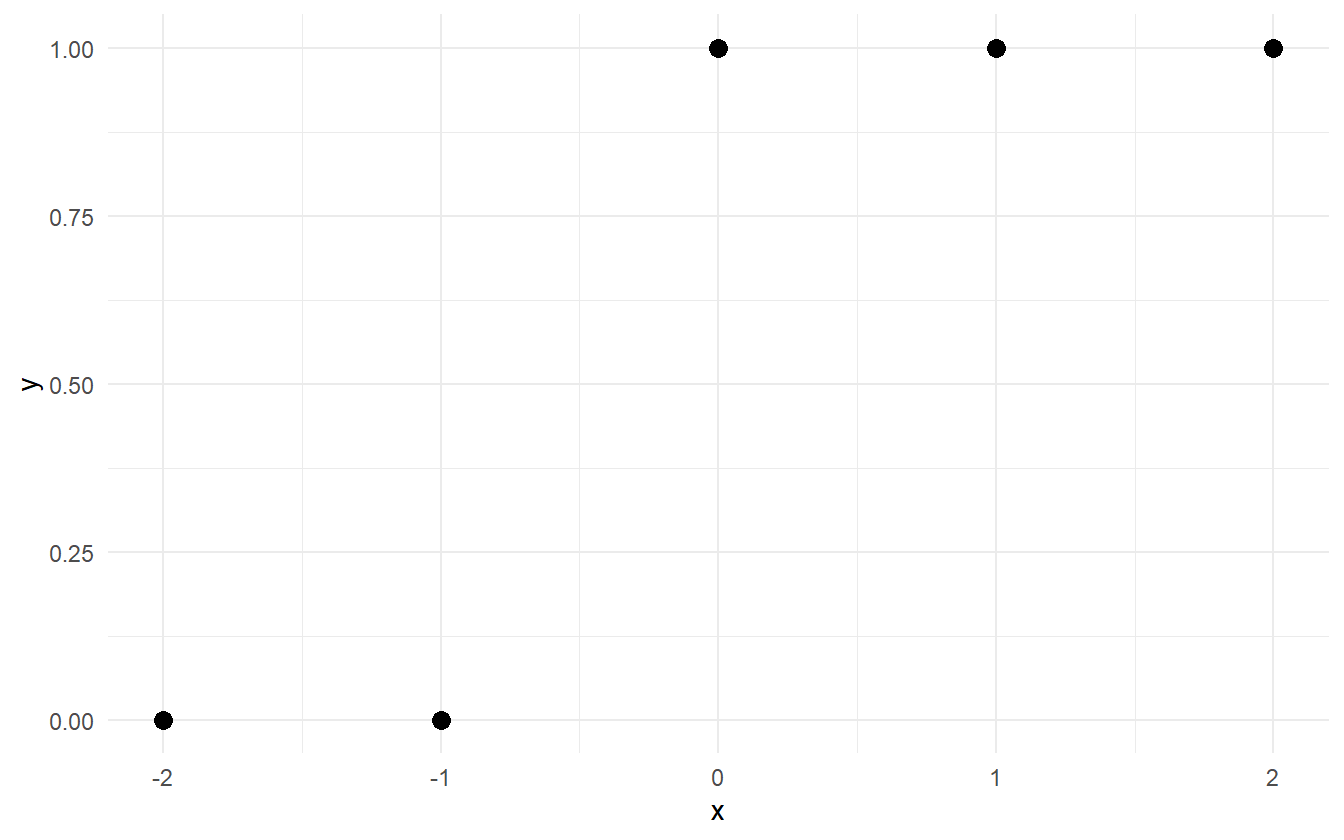
\includegraphics[width=0.85\linewidth]{030-methods_files/figure-latex/ch030-comp-sep-1} 

}

\caption{Example of complete separation in the data. All of the `0`-responses can be separated from the `1`-responses by some value of `x` between `-1` and `0`.}\label{fig:ch030-comp-sep}
\end{figure}

For a slope-intercept model, the MLE for the slope is infinity, and the location is undefined. Figure \ref{fig:ch030-mle-comp-sep} displays a grid of log-likelihoods for a range of scale (inverse slope) and location parameters. The log-likelihood increases to zero as the scale decreases to zero (slope increases to infinity). Numerical root finding methods will converge after a finite number of iterations -- usually by a stopping condition such as the difference in log-likelihoods between steps.

\begin{figure}

{\centering 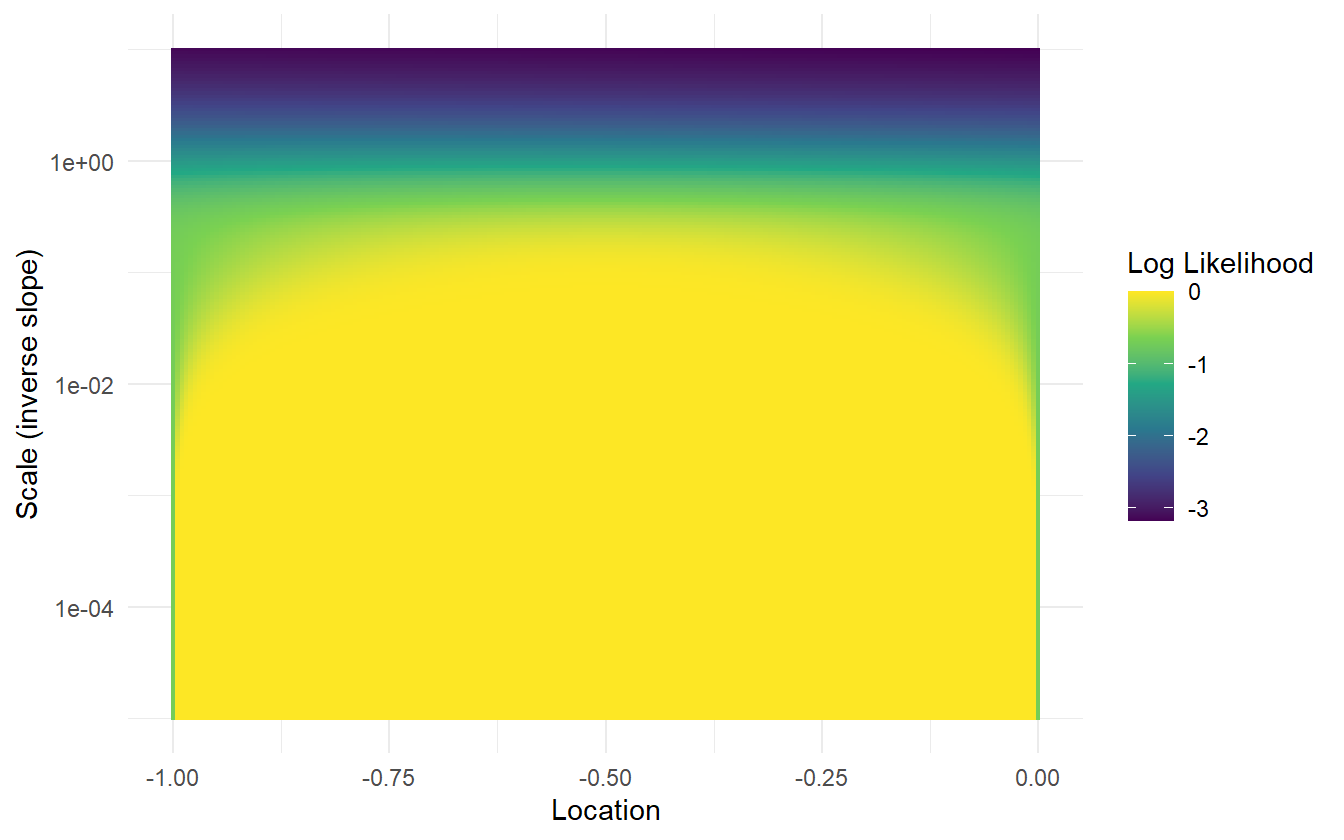
\includegraphics[width=0.85\linewidth]{030-methods_files/figure-latex/ch030-mle-comp-sep-1} 

}

\caption{Grid of log-likelihoods for the completely separable data. The log-likelihood increases to zero as the scale decreases to zero (slope increases to infinity). For smaller slopes, the MLE for the location is `0.5` -- the median of the inner-most datum from each class. At larger slopes, the MLE for the location matters little.}\label{fig:ch030-mle-comp-sep}
\end{figure}

When the separable data from above is fit using \texttt{R}'s \texttt{glm} function, there is a warning about fitted probabilities being \(0\) or \(1\), indicating that the slope is very steep.

\setstretch{1.0}

\begin{Shaded}
\begin{Highlighting}[]
\NormalTok{fit }\OtherTok{\textless{}{-}} \FunctionTok{glm}\NormalTok{(y }\SpecialCharTok{\textasciitilde{}}\NormalTok{ x, }\AttributeTok{family =} \FunctionTok{binomial}\NormalTok{(}\StringTok{"logit"}\NormalTok{))}
\CommentTok{\#\textgreater{} Warning: glm.fit: fitted probabilities numerically 0 or 1 occurred}
\FunctionTok{coefficients}\NormalTok{(fit)}
\CommentTok{\#\textgreater{} (Intercept)           x }
\CommentTok{\#\textgreater{}       22.89       45.97}
\end{Highlighting}
\end{Shaded}

\setstretch{2.0}

The coefficients of the linear predictor are in slope-intercept form (\(23 + 46 x\)). Rearranging the coefficients into location-scale form yields:

\begin{equation}
  \theta = \frac{x - (-0.5)}{1/46}
  \label{eq:rglmmle}
\end{equation}

However, this is not the true maximum likelihood estimate. Table \ref{tab:ch030-Quality-Surreal-Street} shows that the log-likelihood is still increasing as the scale decreases to zero. The change between \(-2.05\times 10^{-10}\) and \(-3.86\times10^{-22}\) is very large on a relative scale, but computers cannot tell the difference on an absolute scale. The precision of most modern computers is around \(10^{-15}\), and anything smaller is treated as numerically zero.

\begin{table}[!h]

\caption{\label{tab:ch030-Quality-Surreal-Street}Log-likelihood estimates for different scale parameters. *Indicates the MLE solution from R.}
\centering
\begin{tabular}[t]{ll}
\toprule
Scale & Log-Likelihood\\
\midrule
1/10 & -1.34e-02\\
1/46* & -2.05e-10\\
1/100 & -3.86e-22\\
1/1000 & -1.42e-217\\
\bottomrule
\end{tabular}
\end{table}

Using a weakly-informative prior for the slope instead of the non-informative uniform distribution will allow for a proper MAP estimate, but care should be taken to consider what prior is appropriate, or why the data is separable in the first place. If an experiment can be improved to avoid the situation, that should be the first action.

The models in this paper rely on MCMC techniques to sample from the posterior distribution. In certain models, the posterior distribution takes on a familiar form given a specific prior distribution. These conjugate likelihood-priors exist for some exponential family models, like for the binomial-beta, Poisson-gamma, and gamma-gamma. The benefit of conjugate prior models are that they do not require computationally expensive sampling techniques to derive the posterior distribution. \citet{chen2003conjugate} discuss conjugate priors for GLMs by specifying a prior for the scale (strength of belief in the prior) and for the observed data, \(y_o\), and then relates the prior in \(y_o\) to the parameters, \(\beta\). This methodology can be convenient, but limits model flexibility.

\hypertarget{multilevel-modeling}{%
\section{Multilevel modeling}\label{multilevel-modeling}}

In classical regression, a simple single-level slope-intercept model can be specified as:

\begin{equation}
y_i = \alpha + \beta x_i + \epsilon_i
\label{eq:single-level-fixed}
\end{equation}

The slope and intercept is fixed for all observations in the data set. If there is a categorical variable with \(J\) levels, then a varying-slope varying-intercept (or simply varying effects) model can be specified as:

\begin{equation}
y_i = \alpha_{j[i]} + \beta_{j[i]} x_i + \epsilon_i
\label{eq:single-level-fixed-varying}
\end{equation}

where \(j[i]\) indexes the group for observation \(i\). In a multilevel model, the coefficients are modeled by a separate regression:

\setstretch{1.0}

\begin{equation}
\begin{split}
y_i &= \alpha_{j[i]} + \beta_{j[i]} x_i \\
\alpha_j &\sim \mathcal{N}(a_0 + a_1 u_j, \sigma_{\alpha}^2) \\
\beta_j &\sim \mathcal{N}(b_0 + b_1 u_j, \sigma_{\beta}^2) \\
\end{split}
\label{eq:multilevel-varying}
\end{equation}
\setstretch{2.0}

In \eqref{eq:multilevel-varying}, \(x\) is a population level predictor, and \(u\) is a group level predictor. Equations \eqref{eq:single-level-fixed} and \eqref{eq:single-level-fixed-varying} represent the two extremes of excluding a categorical variable from a model (complete pooling) and fitting a regression coefficient for each level in the categorical variable (no pooling). Multilevel modeling provides a compromise between these two extremes, resulting in partial pooling estimates.

For a simple intercept-only model, the partial pooling estimate of the intercept, \(\hat{\alpha}_j\) is a weighted average of the mean of the of the observations in the group (no pooling estimate, \(\bar{y}_j\)) and the mean over all groups (complete pooling estimate, \(\bar{y}\)):

\[
\hat{\alpha}_j \approx \frac{\frac{n_j}{\sigma_y^2} \bar{y}_j + \frac{1}{\sigma_\alpha^2} \bar{y}}{\frac{n_j}{\sigma_y^2} + \frac{1}{\sigma_\alpha^2}}
\]

where \(n_j\) is the number of observations in group level \(j\), \(\sigma_y^2\) is the within-group variance, and \(\sigma_\alpha^2\) is the variance between the group level averages. As the between-group variance goes to infinity (or as \(n_j \rightarrow \infty\)), the partial pooling estimates approach the no pooling estimates. When there are fewer samples, the partial pooling estimate is closer to the overall average. In this way, partial pooling reflects the relative information contained within each group. For an in-depth introduction to multilevel modeling, see \citet{gelman2006data}.

\hypertarget{hamiltonian-monte-carlo-and-nuts}{%
\section{Hamiltonian Monte Carlo and NUTS}\label{hamiltonian-monte-carlo-and-nuts}}

We will be using \texttt{Stan} for model fitting throughout this paper. \texttt{Stan} allows for MCMC sampling of Bayesian models using a variant of Hamiltonian Monte Carlo called the No-U-Turn sampler (NUTS). HMC can be though of as a physics simulation: a massless ``particle'' is imparted with a random direction and some amount of kinetic energy in a probability field, and is stopped after a number of steps, \(L\), called leapfrog steps. The stopping point is the new proposal sample. The NUTS algorithm removes the need for leapfrog steps by stopping automatically when the particle begins to double back and retrace its steps \citep{hoffman2014no}. This sampling scheme has a much higher rate of accepted samples, and also comes with many built-in diagnostic tools that let us know when the sampler is having trouble efficiently exploring the posterior.

The NUTS algorithm samples in two phases: a warm-up phase and a sampling phase. During the warm-up phase, the sampler is automatically tuning three internal parameters that can significantly affect the sampling efficiency.

\hypertarget{non-centered-parameterization}{%
\section{Non-centered parameterization}\label{non-centered-parameterization}}

Because HMC is a physics simulation, complicated geometry or posteriors with steep slopes can be difficult to traverse if the step size is too course. The solution is to explore a simpler geometry, and then transform the sample into the target distribution. Reparameterization is especially important for hierarchical models. For \texttt{Stan}, sampling from a standard normal or uniform distribution is very easy, and so the non-centered parameterization can alleviate divergent transitions. Here we present three reparameterizations that we use in the next chapter. The left-hand side shows the centered parameterization, and the right-hand side shows the non-centered parameterization.

\textbf{Gaussian distribution} with mean \(\mu\) and standard deviation \(\sigma\):

\setstretch{1.0}

\begin{equation}
  \begin{split}
    X &\sim \mathcal{N}(\mu, \sigma^2)
  \end{split}
\quad \Longrightarrow \quad
  \begin{split}
    Z &\sim \mathcal{N}(0, 1^2) \\
    X &= \mu + \sigma \cdot Z
  \end{split}
\label{eq:nc-normal}
\end{equation}
\setstretch{2.0}

\textbf{Log-Normal distribution} with mean-log \(\mu\) and standard deviation-log \(\sigma\):

\setstretch{1.0}

\begin{equation}
  \begin{split}
    X &\sim \mathrm{Lognormal}(\mu, \sigma^2)
  \end{split}
\quad \Longrightarrow \quad
  \begin{split}
    Z &\sim \mathcal{N}(0, 1^2) \\
    X &= \exp\left(\mu + \sigma \cdot Z\right)
  \end{split}
\label{eq:nc-lognormal}
\end{equation}
\setstretch{2.0}

\textbf{Cauchy distribution} with location \(\mu\) and scale \(\tau\):

\setstretch{1.0}

\begin{equation}
  \begin{split}
    X &\sim \mathrm{Cauchy}(\mu, \tau)
  \end{split}
\quad \Longrightarrow \quad
  \begin{split}
    U &\sim \mathcal{U}\left(-\frac{\pi}{2}, \frac{\pi}{2}\right) \\
    X &= \mu + \tau \cdot \tan(U)
  \end{split}
\label{eq:nc-cauchy}
\end{equation}
\setstretch{2.0}

\hypertarget{model-checking}{%
\section{Methods for model checking}\label{model-checking}}

Below is the 8 Schools data \citep{gelman2013bayesian} which is a standard textbook example for introducing multilevel modeling. Here we use it to illustrate essential MCMC model checking tools.

\begin{Shaded}
\begin{Highlighting}[]
\NormalTok{schools\_dat }\OtherTok{\textless{}{-}} \FunctionTok{list}\NormalTok{(}
  \AttributeTok{J =} \DecValTok{8}\NormalTok{,}
  \AttributeTok{y =} \FunctionTok{c}\NormalTok{(}\DecValTok{28}\NormalTok{,  }\DecValTok{8}\NormalTok{, }\SpecialCharTok{{-}}\DecValTok{3}\NormalTok{,  }\DecValTok{7}\NormalTok{, }\SpecialCharTok{{-}}\DecValTok{1}\NormalTok{,  }\DecValTok{1}\NormalTok{, }\DecValTok{18}\NormalTok{, }\DecValTok{12}\NormalTok{),}
  \AttributeTok{sigma =} \FunctionTok{c}\NormalTok{(}\DecValTok{15}\NormalTok{, }\DecValTok{10}\NormalTok{, }\DecValTok{16}\NormalTok{, }\DecValTok{11}\NormalTok{,  }\DecValTok{9}\NormalTok{, }\DecValTok{11}\NormalTok{, }\DecValTok{10}\NormalTok{, }\DecValTok{18}\NormalTok{)}
\NormalTok{)}
\end{Highlighting}
\end{Shaded}

\textbf{Trace Plots.} Trace plots have been used since the conception of MCMC to assess chain sampling efficiency and quality. They are visual aids that let the practitioner asses the qualitative health of the chains, looking for properties such as autocorrelation, heteroskedacity, non-stationarity, and convergence. Healthy chains are well-mixed and stationary. It's often better to run more chains during the model building process so that issues with mixing and convergence can be diagnosed sooner. One unhealthy chain can be indicative of a poorly specified model. The addition of more chains also contributes to the estimation of the split \(\hat{R}\) statistic (discussed below). Figure \ref{fig:ch030-Brave-Moose} shows what a set of healthy chains looks like -- the chains are nearly indistinguishable, fluctuate around the same mean, and do not show any long periods of being in the same location.

\begin{figure}

{\centering 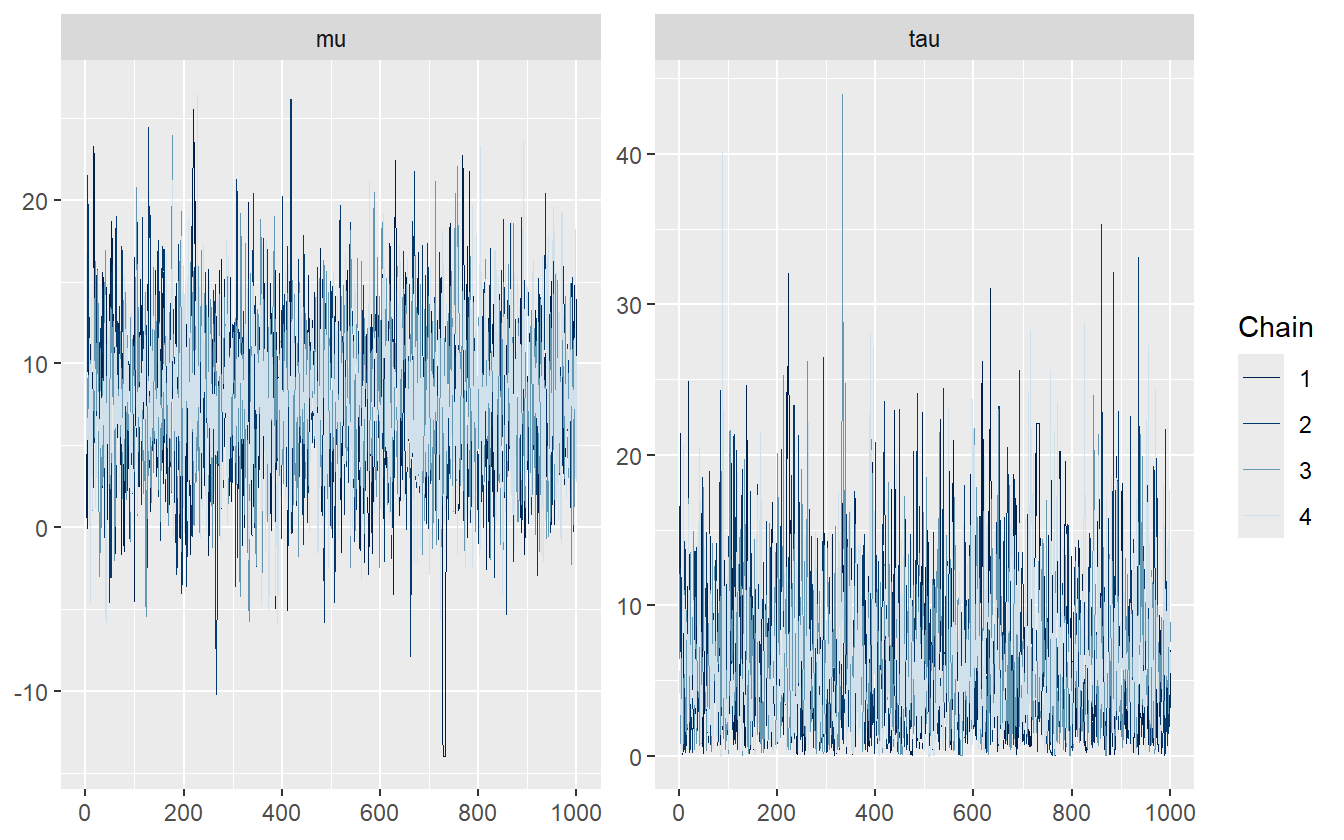
\includegraphics[width=0.85\linewidth]{030-methods_files/figure-latex/ch030-Brave-Moose-1} 

}

\caption{An example of healthy chains.}\label{fig:ch030-Brave-Moose}
\end{figure}

As the number of parameters in a model grows, it becomes exceedingly tedious to check the trace plots of all parameters, and so numerical summaries are helpful to flag potential issues within the model.

\textbf{R-hat Statistic.} The most common summary statistic for chain health is the potential scale reduction factor \citep{gelman1992inference} that measures the ratio of between chain variance and within chain variance. When the two have converged, the ratio is one. We've shared examples of healthy chains which would also have healthy \(\hat{R}\) values, but it's valuable to also share an example of a bad model.

The initial starting parameters for this model are intentionally set to vary between \(-10\) and \(10\) -- in contrast to the default range of \((-2, 2)\) -- and with only a few samples drawn in order to artificially drive up the split \(\hat{R}\) statistic. The model is provided as supplementary code in the \protect\hyperlink{code}{appendix}.

\setstretch{1.0}

\begin{Shaded}
\begin{Highlighting}[]
\NormalTok{fit\_cp }\OtherTok{\textless{}{-}} \FunctionTok{sampling}\NormalTok{(schools\_cp, }\AttributeTok{data =}\NormalTok{ schools\_dat, }\AttributeTok{refresh =} \DecValTok{0}\NormalTok{,}
                   \AttributeTok{iter =} \DecValTok{40}\NormalTok{, }\AttributeTok{init\_r =} \DecValTok{10}\NormalTok{, }\AttributeTok{seed =} \DecValTok{671254821}\NormalTok{)}
\end{Highlighting}
\end{Shaded}

\setstretch{2.0}

\texttt{Stan} warns about many different issues with this model, but the R-hat is the one of interest. The largest is \(1.71\) which is incredibly large. Gelmen suggests using a threshold of \(1.10\) to flag unhealthy chains.

\begin{center}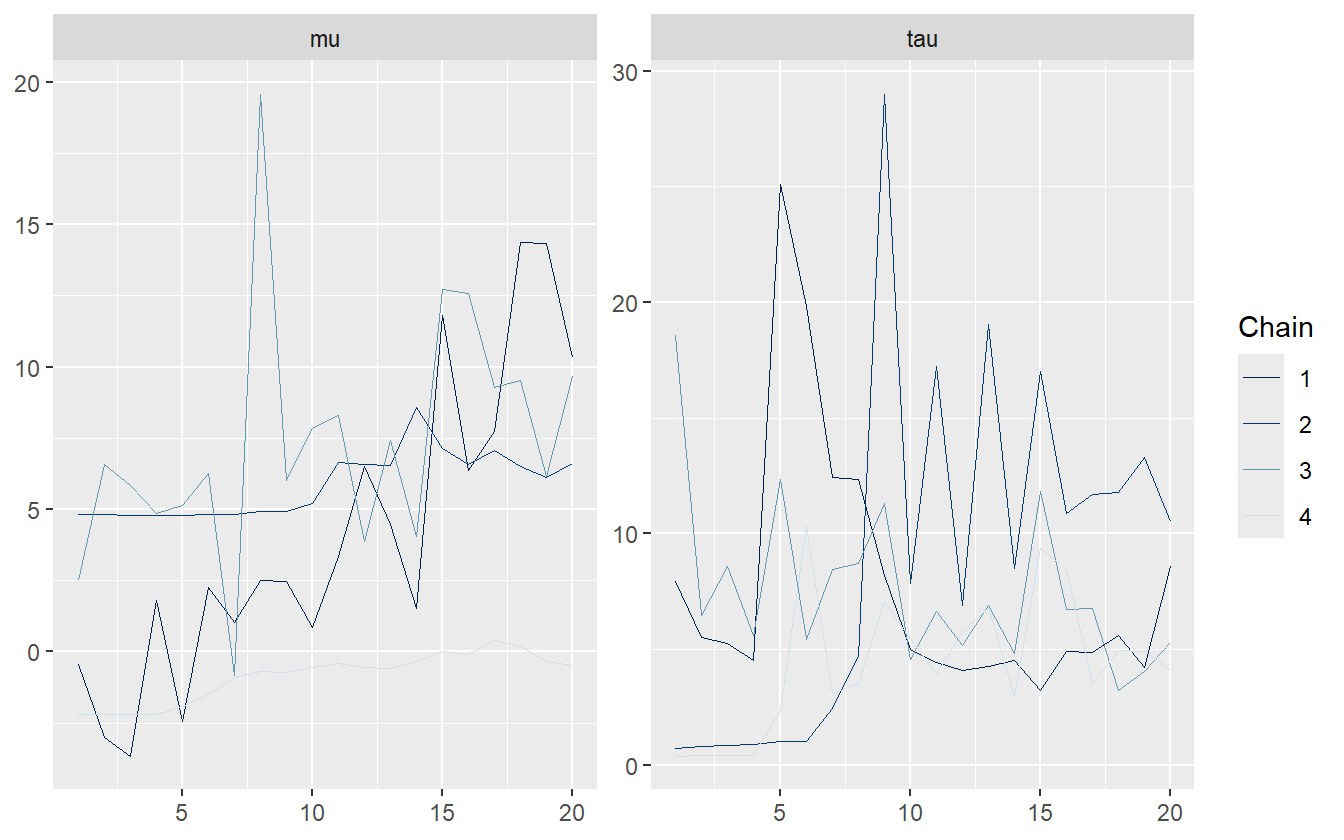
\includegraphics[width=0.85\linewidth]{030-methods_files/figure-latex/ch030-Rocky-Test-1} \end{center}

These chains do not look good at all -- they have not converged to a stationary distribution. This is by design, however, as only 40 samples were simulated. The \(\hat{R}\) values are listed in table \ref{tab:ch030-Ninth-Finger}.

\begin{table}[!h]

\caption{\label{tab:ch030-Ninth-Finger}Split R-hat values from the 8 Schools example.}
\centering
\begin{tabular}[t]{lr}
\toprule
Parameter & Rhat\\
\midrule
mu & 1.709\\
tau & 1.169\\
\bottomrule
\end{tabular}
\end{table}

To calculate the (non split) \(\hat{R}\), first calculate the between-chain variance, and then the average chain variance. For \(M\) independent Markov chains, \(\{\theta_1, \ldots \theta_M\}\), with \(N\) samples each, the between-chain variance is:

\setstretch{1.0}

\[
B = \frac{N}{M-1}\sum_{m=1}^{M}\left(\bar{\theta}_m - \bar{\theta}\right)^2
\]

where

\[
\bar{\theta}_m = \frac{1}{N}\sum_{n=1}^{N}\theta_{m}^{(n)}
\]

and

\[
\bar{\theta} = \frac{1}{M}\sum_{m=1}^{M}\bar{\theta}_m
\]

The within-chain variance, \(W\), is the variance averaged over all the chains:

\[
W = \frac{1}{M}\sum_{m=1}^{M} s_{m}^2
\]

where

\[
s_{m}^2 = \frac{1}{N-1}\sum_{n=1}^{N}\left(\theta_{m}^{(n)} - \bar{\theta}_m\right)^2
\]
\setstretch{2.0}

The weighted mixture of the within-chain and cross-chain variation is:

\setstretch{1.0}

\[
\hat{var} = \frac{N-1}{N} W + \frac{1}{N} B
\]

and finally the \(\hat{R}\) statistic is:

\[
\hat{R} = \sqrt{\frac{\hat{var}}{W}}
\]

Here is the calculation in \texttt{R}:

\begin{Shaded}
\begin{Highlighting}[]
\NormalTok{param }\OtherTok{\textless{}{-}} \StringTok{"mu"}
\NormalTok{theta }\OtherTok{\textless{}{-}}\NormalTok{ p\_cp[,,param]}
\NormalTok{N     }\OtherTok{\textless{}{-}} \FunctionTok{nrow}\NormalTok{(theta)}
\NormalTok{M     }\OtherTok{\textless{}{-}} \FunctionTok{ncol}\NormalTok{(theta)}

\NormalTok{theta\_bar\_m }\OtherTok{\textless{}{-}} \FunctionTok{colMeans}\NormalTok{(theta)}
\NormalTok{theta\_bar   }\OtherTok{\textless{}{-}} \FunctionTok{mean}\NormalTok{(theta\_bar\_m)}

\NormalTok{B }\OtherTok{\textless{}{-}}\NormalTok{ N }\SpecialCharTok{/}\NormalTok{ (M }\SpecialCharTok{{-}} \DecValTok{1}\NormalTok{) }\SpecialCharTok{*} \FunctionTok{sum}\NormalTok{((theta\_bar\_m }\SpecialCharTok{{-}}\NormalTok{ theta\_bar)}\SpecialCharTok{\^{}}\DecValTok{2}\NormalTok{)}
\NormalTok{s\_sq\_m }\OtherTok{\textless{}{-}} \FunctionTok{apply}\NormalTok{(theta, }\DecValTok{2}\NormalTok{, var)}

\NormalTok{W }\OtherTok{\textless{}{-}} \FunctionTok{mean}\NormalTok{(s\_sq\_m)}
\NormalTok{var\_hat }\OtherTok{\textless{}{-}}\NormalTok{ W }\SpecialCharTok{*}\NormalTok{ (N }\SpecialCharTok{{-}} \DecValTok{1}\NormalTok{) }\SpecialCharTok{/}\NormalTok{ N }\SpecialCharTok{+}\NormalTok{ B }\SpecialCharTok{/}\NormalTok{ N}

\NormalTok{(mu\_Rhat }\OtherTok{\textless{}{-}} \FunctionTok{sqrt}\NormalTok{(var\_hat }\SpecialCharTok{/}\NormalTok{ W))}
\CommentTok{\#\textgreater{} [1] 1.409}
\end{Highlighting}
\end{Shaded}

\setstretch{2.0}

The \(\hat{R}\) statistic is smaller than the split \(\hat{R}\) value provided by \texttt{Stan}. This is a consequence of steadily increasing or decreasing chains. The split value does what it sounds like, and splits the samples from the chains in half -- effectively doubling the number of chains and halving the number of samples per chain. In this way, the measure is more robust in detecting unhealthy chains. This also highlights the utility in using both visual and statistical tools to evaluate models. Here is the calculation of the split \(\hat{R}\):

\setstretch{1.0}

\begin{Shaded}
\begin{Highlighting}[]
\NormalTok{param }\OtherTok{\textless{}{-}} \StringTok{"mu"}
\NormalTok{theta\_tmp }\OtherTok{\textless{}{-}}\NormalTok{ p\_cp[,,param]}
\NormalTok{theta }\OtherTok{\textless{}{-}} \FunctionTok{cbind}\NormalTok{(theta\_tmp[}\DecValTok{1}\SpecialCharTok{:}\DecValTok{10}\NormalTok{,], theta\_tmp[}\DecValTok{11}\SpecialCharTok{:}\DecValTok{20}\NormalTok{,])}
\NormalTok{N     }\OtherTok{\textless{}{-}} \FunctionTok{nrow}\NormalTok{(theta)}
\NormalTok{M     }\OtherTok{\textless{}{-}} \FunctionTok{ncol}\NormalTok{(theta)}

\NormalTok{theta\_bar\_m }\OtherTok{\textless{}{-}} \FunctionTok{colMeans}\NormalTok{(theta)}
\NormalTok{theta\_bar   }\OtherTok{\textless{}{-}} \FunctionTok{mean}\NormalTok{(theta\_bar\_m)}

\NormalTok{B }\OtherTok{\textless{}{-}}\NormalTok{ N }\SpecialCharTok{/}\NormalTok{ (M }\SpecialCharTok{{-}} \DecValTok{1}\NormalTok{) }\SpecialCharTok{*} \FunctionTok{sum}\NormalTok{((theta\_bar\_m }\SpecialCharTok{{-}}\NormalTok{ theta\_bar)}\SpecialCharTok{\^{}}\DecValTok{2}\NormalTok{)}
\NormalTok{s\_sq\_m }\OtherTok{\textless{}{-}} \FunctionTok{apply}\NormalTok{(theta, }\DecValTok{2}\NormalTok{, var)}

\NormalTok{W }\OtherTok{\textless{}{-}} \FunctionTok{mean}\NormalTok{(s\_sq\_m)}
\NormalTok{var\_hat }\OtherTok{\textless{}{-}}\NormalTok{ W }\SpecialCharTok{*}\NormalTok{ (N }\SpecialCharTok{{-}} \DecValTok{1}\NormalTok{) }\SpecialCharTok{/}\NormalTok{ N }\SpecialCharTok{+}\NormalTok{ B }\SpecialCharTok{/}\NormalTok{ N}

\NormalTok{(mu\_Rhat }\OtherTok{\textless{}{-}} \FunctionTok{sqrt}\NormalTok{(var\_hat }\SpecialCharTok{/}\NormalTok{ W))}
\CommentTok{\#\textgreater{} [1] 1.709}
\end{Highlighting}
\end{Shaded}

\setstretch{2.0}

We've successfully replicated the calculation of the split \(\hat{R}\). \citet{vehtari2020rank} propose an improved rank-normalized \(\hat{R}\) for assessing the convergence of MCMC chains, and also suggest using a threshold of \(1.01\).

\textbf{Effective Sample Size.} Samples from Markov Chains are typically autocorrelated, which can increase uncertainty of posterior estimates. The solution is generally to reparameterize the model to avoid steep log-posterior densities. When the HMC algorithm is exploring difficult geometry, it can get stuck in regions of high densities, which means that there is more correlation between successive samples. Equation \eqref{eq:schools-ncp} shows the centered (left) and non-centered (right) parameterization of the 8-Schools model, and the benefit of reparameterization is conveyed by the ratio of effective sample size to actual sample size in figure \ref{fig:ch030-Timely-Nitrogen}.

\setstretch{1.0}

\begin{equation}
  \begin{split}
    \sigma &\sim \mathcal{U}(0, \infty) \\
    \mu &\sim \mathcal{N}(0, 10) \\
    \tau &\sim \mathrm{HalfCauchy}(0, 10) \\
    \theta &\sim \mathcal{N}(\mu, \tau) \\
    y &\sim \mathcal{N}(\theta, \sigma)
  \end{split}
\quad \Longrightarrow \quad
  \begin{split}
    \sigma &\sim \mathcal{U}(0, \infty) \\
    \mu &\sim \mathcal{N}(0, 10) \\
    \tau &\sim \mathrm{HalfCauchy}(0, 10) \\
    \eta &\sim \mathcal{N}(0, 1) \\
    \theta &= \mu + \tau \cdot \eta \\
    y &\sim \mathcal{N}(\theta, \sigma)
  \end{split}
\label{eq:schools-ncp}
\end{equation}
\setstretch{2.0}

\begin{figure}

{\centering 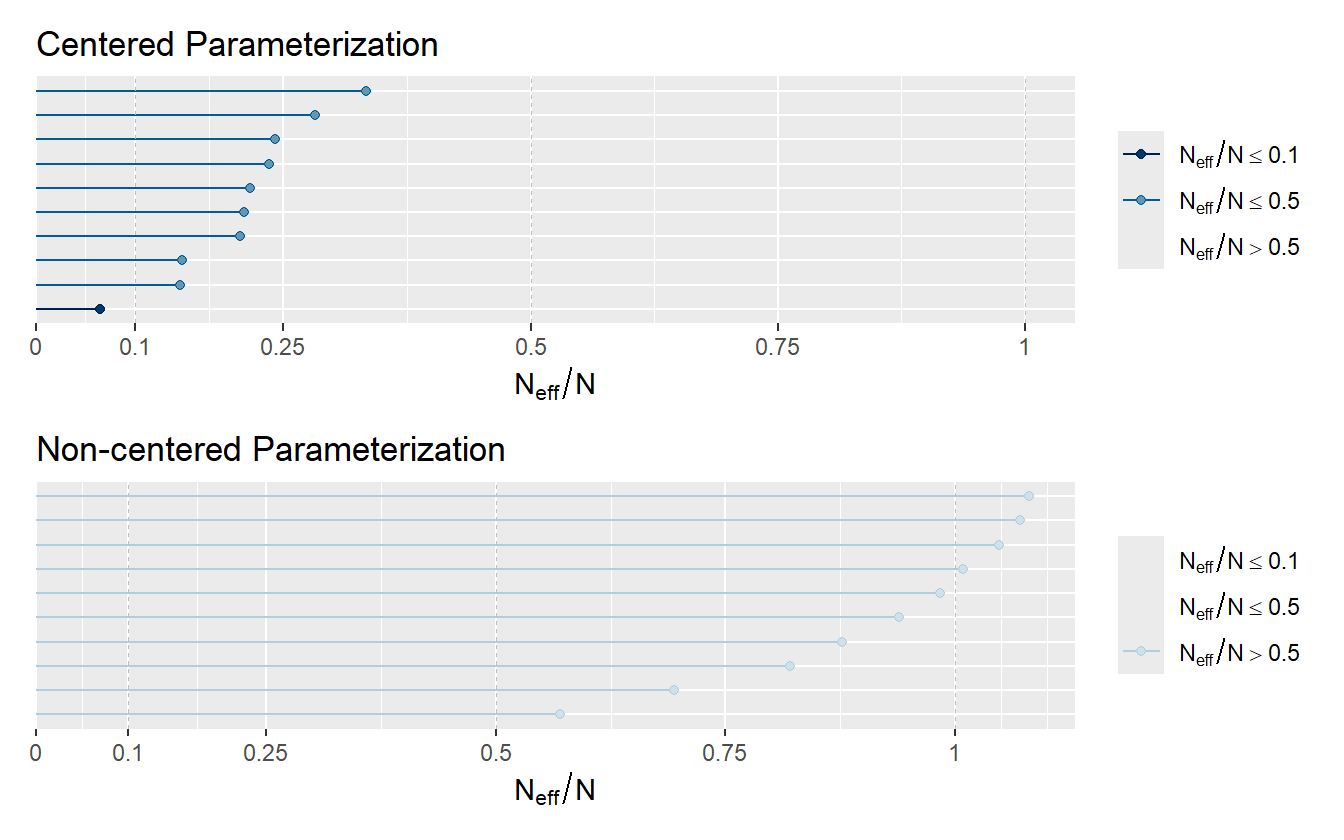
\includegraphics[width=0.85\linewidth]{030-methods_files/figure-latex/ch030-Timely-Nitrogen-1} 

}

\caption{Ratio of N\_eff to actual sample size. Low ratios imply high autocorrelation which can be alleviated by reparameterizing the model or by thinning.}\label{fig:ch030-Timely-Nitrogen}
\end{figure}

As the strength of autocorrelation generally decreases at larger lags, a simple prescription to decrease autocorrelation between samples and increase the effective sample size is to use thinning. Thinning means saving every \(k^{th}\) sample and throwing the rest away. If one desired to have 2000 posterior draws, it could be done in two of many possible ways

\begin{itemize}
\tightlist
\item
  Generate 2000 draws after warmup and save all of them
\item
  Generate 10,000 draws after warmup and save every \(5^{th}\) sample.
\end{itemize}

Both will produce 2000 samples, but the method using thinning will have less autocorrelation and a higher effective number of samples. Though it should be noted that generating 10,000 draws and saving all of them will have a higher number of effective samples than the second method with thinning, so thinning should only be favored to save memory.

\textbf{Divergent Transitions.} Unlike the previous tools for algorithmic faithfulness which can be used for any MCMC sampler, information about divergent transitions is intrinsic to Hamiltonian Monte Carlo. Recall that the HMC and NUTS algorithm can be imagined as a physics simulation of a particle in a potential energy field, and a random momentum is imparted on the particle. The sum of the potential energy and the kinetic energy of the system is called the Hamiltonian, and is conserved along the trajectory of the particle \citep{stanref}. The path that the particle takes is a discrete approximation to the actual path where the position of the particle is updated in small steps called leapfrog steps (see \citet{leimkuhler2004simulating} for a detailed explanation of the leapfrog algorithm). A divergent transition happens when the simulated trajectory is far from the true trajectory as measured by the Hamiltonian.

A few divergent transitions is not indicative of a poorly performing model, and often divergent transitions can be mitigated by reducing the step size and increasing the adapt delta parameter. On the other hand, a bad model may never be improved just by tweaking some parameters. This is the folk theorem of statistical computing - if there is a problem with the sampling, blame the model, not the algorithm.

Divergent transitions are never saved in the posterior samples, but they are saved internally to the \texttt{Stan} fit object and can be compared against good samples. Sometimes this can give insight into which parameters and which regions of the posterior the divergent transitions are coming from.

\begin{figure}

{\centering 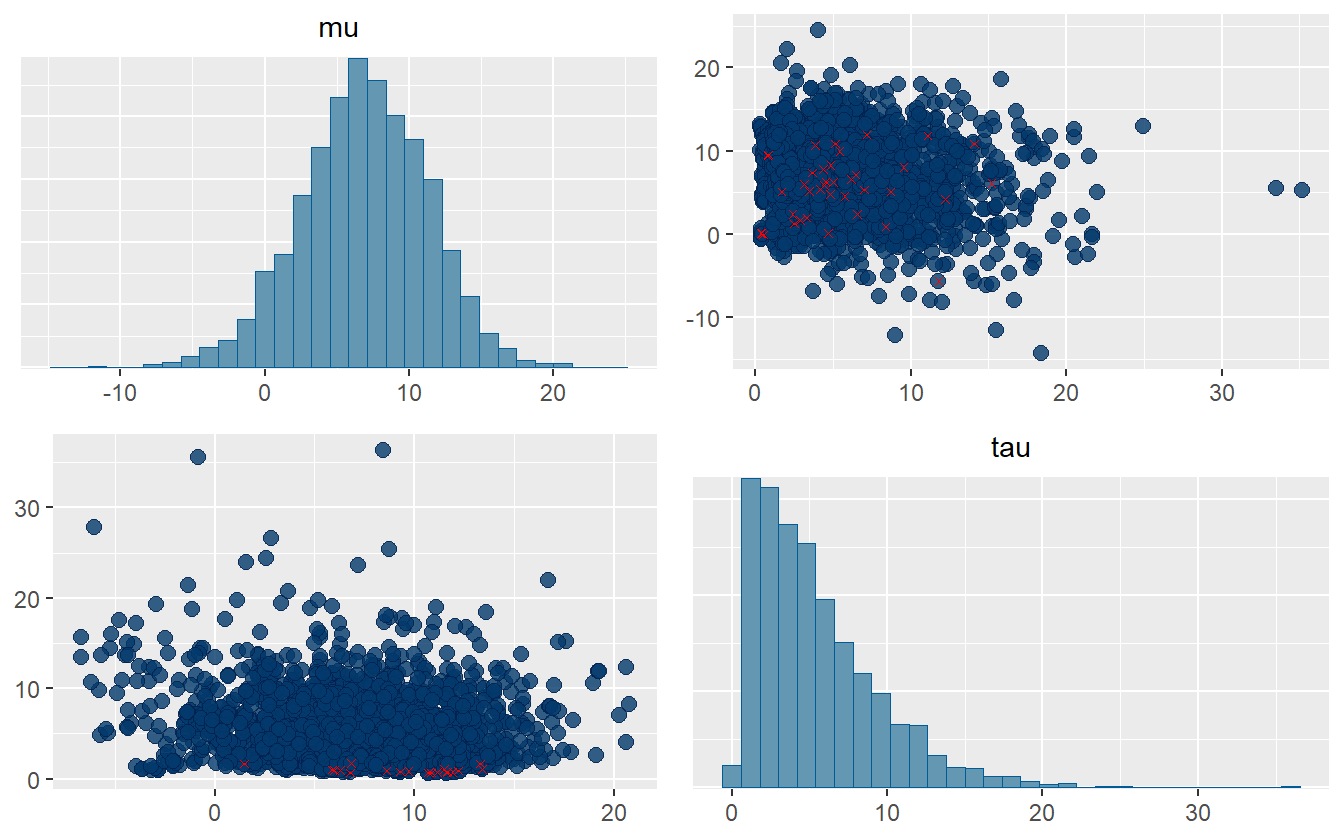
\includegraphics[width=0.85\linewidth]{030-methods_files/figure-latex/ch030-Hot-Locomotive-1} 

}

\caption{Divergent transitions highlighted for some parameters from the centered parameterization of the eight schools example.}\label{fig:ch030-Hot-Locomotive}
\end{figure}

From figure \ref{fig:ch030-Hot-Locomotive} we can see that most of the divergent transitions occur when the variance term \(\tau\) is close to zero. This is common for multilevel models, and illustrates why non-centered parameterization is so important. We discuss centered and non-centered parameterization in the next chapter.

\hypertarget{estimating-predictive-performance}{%
\section{Estimating predictive performance}\label{estimating-predictive-performance}}

All models are wrong, but some are useful. This quote is from George Box \citep{box1976science}, and it is a popular quote that statisticians like to throw around. All models are wrong because it is nearly impossible to account for the minutiae of every process that contributes to an observed phenomenon, and often trying to results in poorer performing models. Also it is never truly possible to prove that a model is correct. At best the scientific method can falsify certain hypotheses, but it cannot ever determine if a model is universally correct. That does not matter. What does matter is if the model is useful and can make accurate predictions.

Why is predictive performance so important? Consider five points of data (figure \ref{fig:ch030-Moving-Moose}). They have been simulated from some polynomial equation of degree less than five, but with no more information other than that, how can the best polynomial model be selected?

\begin{figure}

{\centering 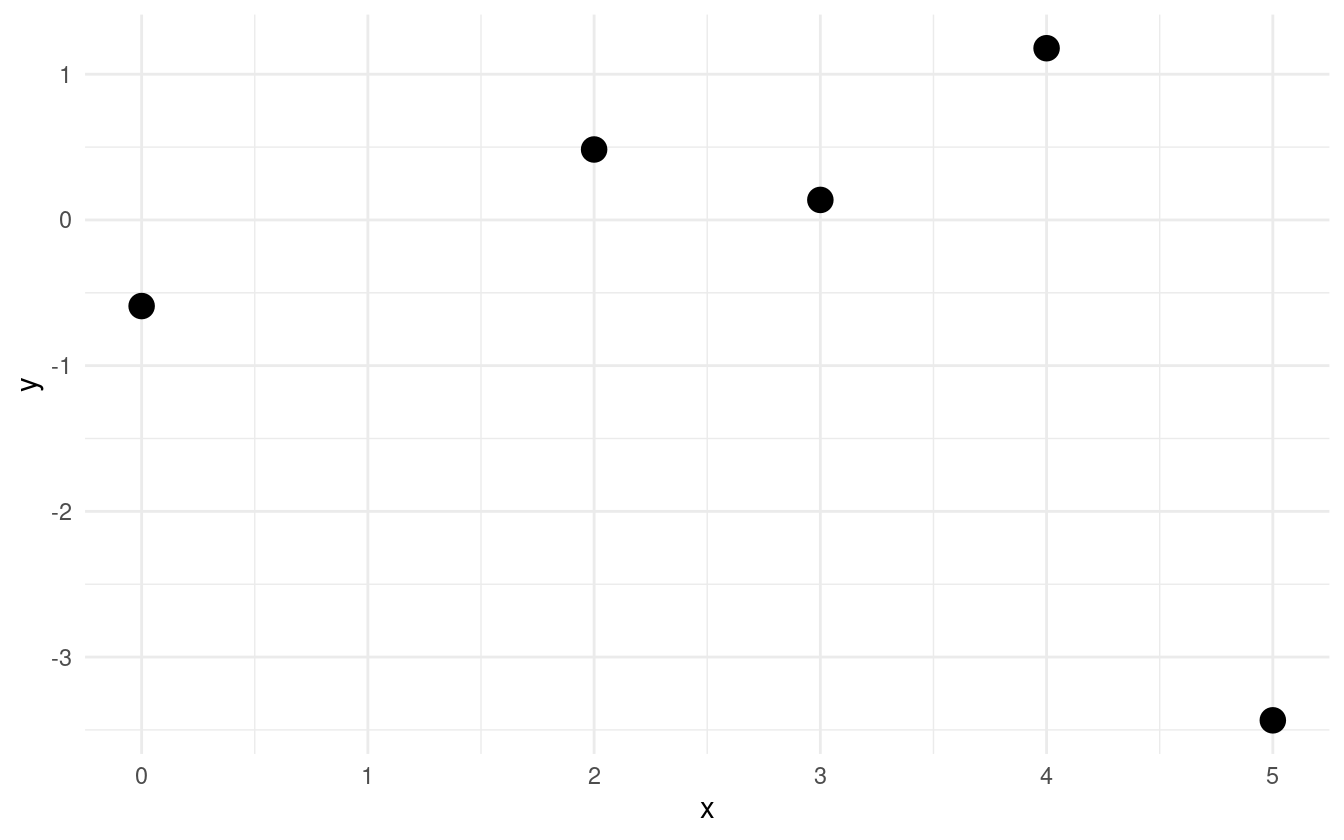
\includegraphics[width=0.85\linewidth]{030-methods_files/figure-latex/ch030-Moving-Moose-1} 

}

\caption{Five points from a polynomial model.}\label{fig:ch030-Moving-Moose}
\end{figure}

One thing to try is fit a handful of linear models, check the parameter's p-values, the \(R^2\) statistic, and perform other goodness of fit tests, but there is a problem. As the degree of the polynomial fit increases, the \(R^2\) statistic will always increase. In fact with five data points, a fourth degree polynomial will fit the data perfectly (figure \ref{fig:ch030-Olive-Screwdriver}).

\begin{figure}

{\centering 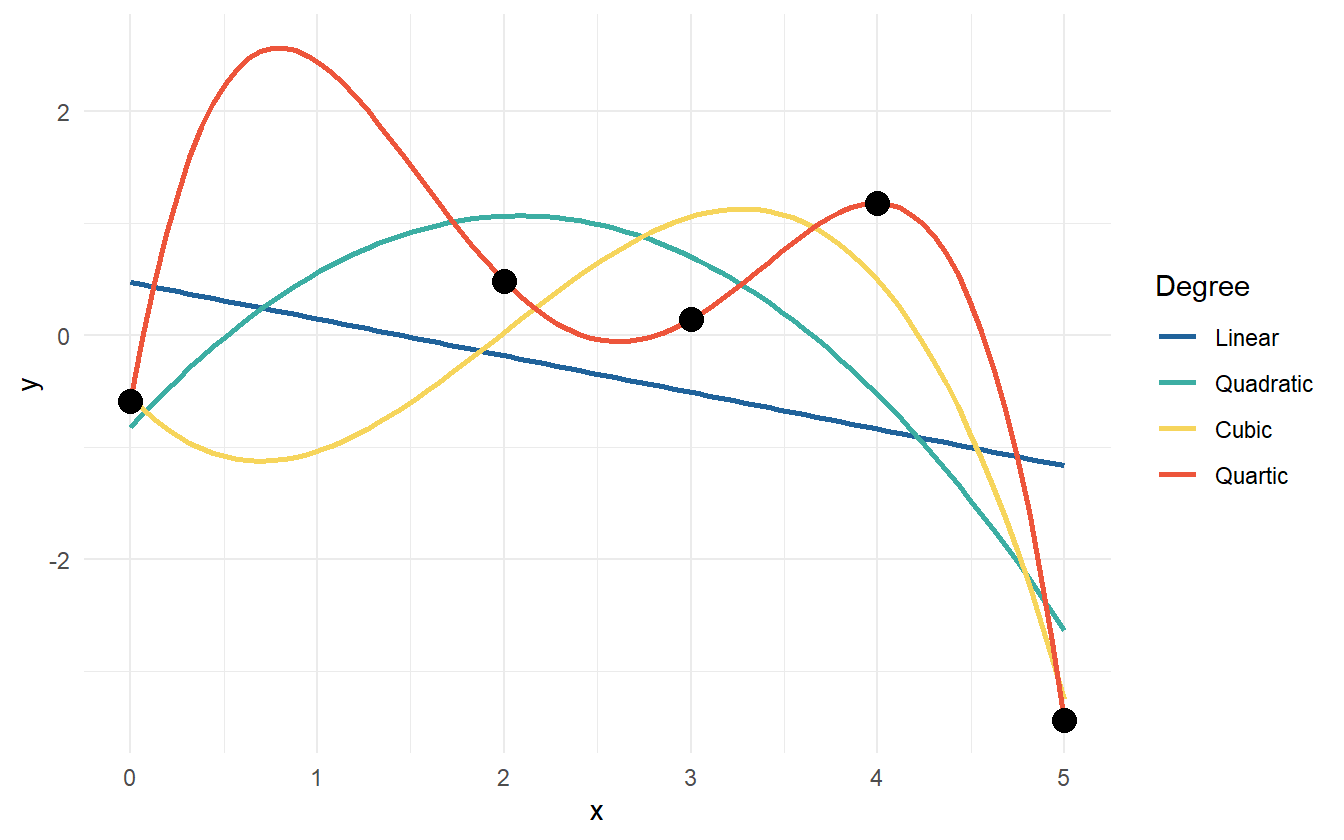
\includegraphics[width=0.85\linewidth]{030-methods_files/figure-latex/ch030-Olive-Screwdriver-1} 

}

\caption{Data points with various polynomial regression lines.}\label{fig:ch030-Olive-Screwdriver}
\end{figure}

If a \(6^{th}\) point were to be added -- a new observation -- which of the models would be expected to predict best? Can it be estimated which model will predict best before testing with new data? One guess is that the quadratic or cubic model will do well because because the linear model is potentially underfit to the data and the quartic is overfit to the data. Figure \ref{fig:ch030-Cold-Fish} shows the new data point from the polynomial model. Now the linear and cubic models are trending in the wrong direction. The quadratic and quartic models are both trending down, so perhaps they may be the correct form for the model.

\begin{figure}

{\centering 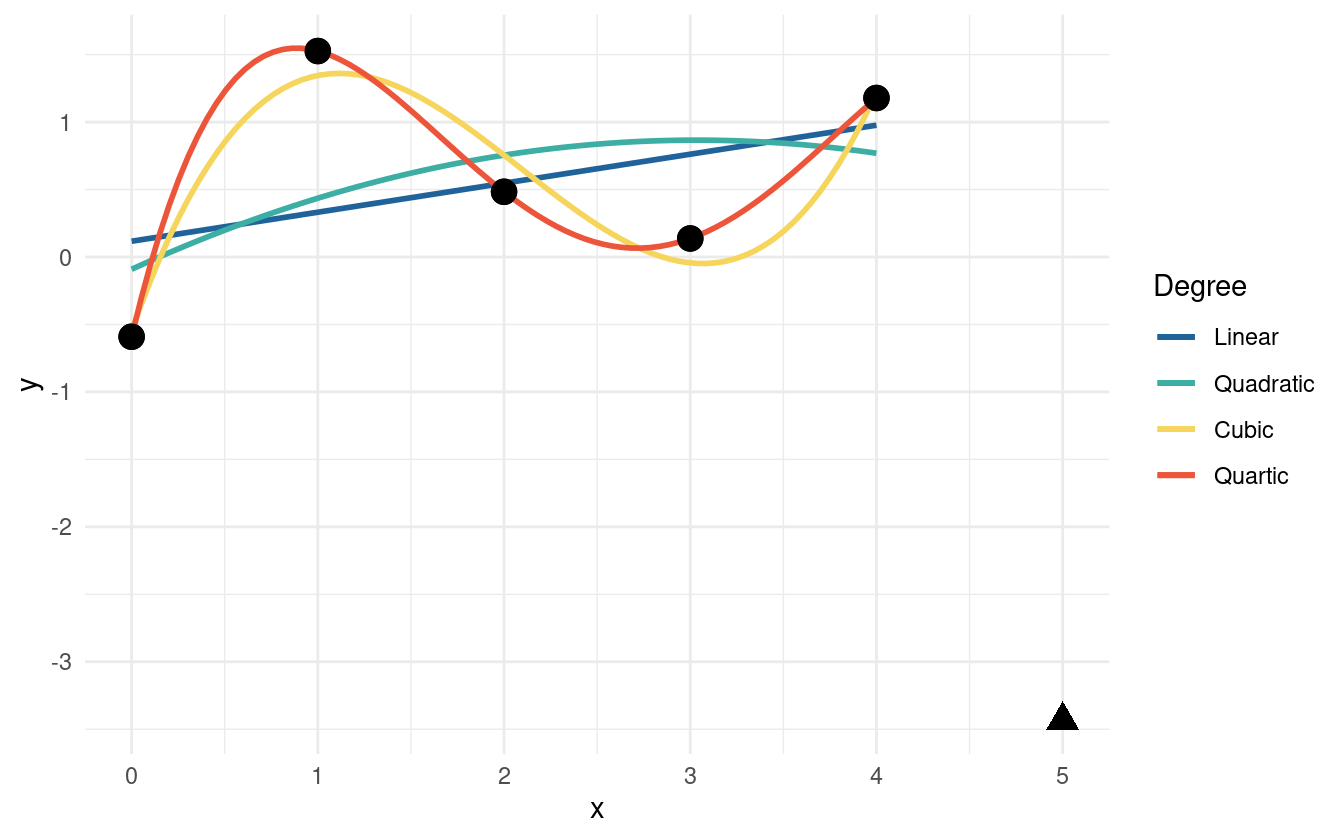
\includegraphics[width=0.85\linewidth]{030-methods_files/figure-latex/ch030-Cold-Fish-1} 

}

\caption{The fitted polynomial models with a new observation.}\label{fig:ch030-Cold-Fish}
\end{figure}

Figure \ref{fig:ch030-Strawberry-Swallow} shows the 80\% and 95\% prediction intervals for a new observation given \(x = 1\) as well as the true outcome as a dashed line at \(y = 1.527\). The linear model has the smallest prediction interval (PI), but completely misses the target. The remaining three models all include the observed value in their 95\% PIs, but the quadratic model has the smallest PI of the three. The actual data generating polynomial is

\setstretch{1.0}

\begin{align*}
y &\sim \mathcal{N}(\mu, 1^2) \\
\mu &= -0.5(x - 2)^2 + 2
\end{align*}
\setstretch{2.0}

\begin{figure}

{\centering 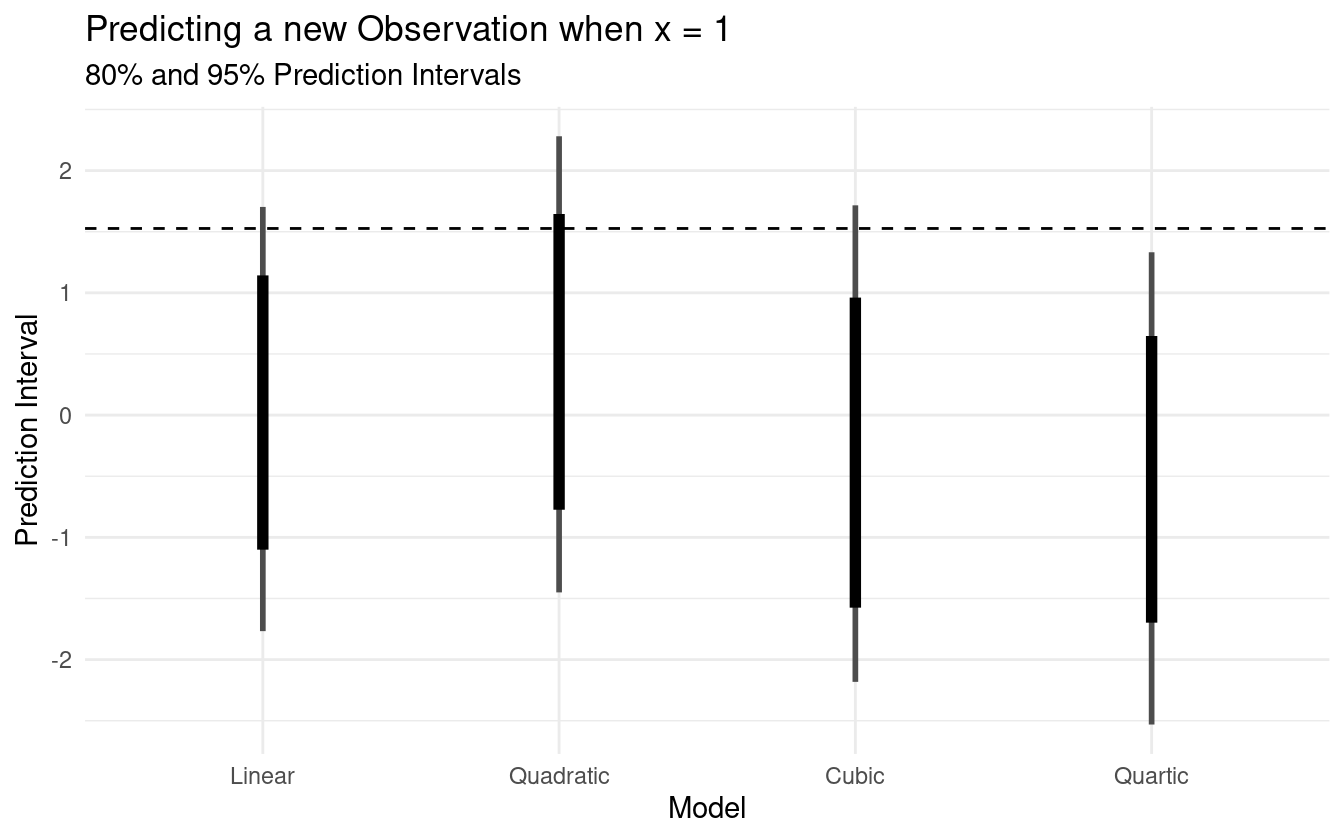
\includegraphics[width=0.85\linewidth]{030-methods_files/figure-latex/ch030-Strawberry-Swallow-1} 

}

\caption{95\% Prediction intervals for the four polynomial models, as well as the true value (dashed line).}\label{fig:ch030-Strawberry-Swallow}
\end{figure}

The best fit to the observed data is the quartic model, but it is too variable and doesn't capture the regular features of the data, so it does poorly for the out-of-sample prediction. The linear model suffers as well by being more biased and too inflexible to capture the structure of the data. The quadratic and cubic are in the middle, but the quadratic does well and makes fewer assumptions about the data. The quadratic model is just complex enough to predict well while making fewer assumptions. Information criteria is a way of weighing the prediction quality of a model against its complexity, and is arguably a better system for model selection/comparison than other goodness-of-fit statistics such as \(R^2\) or p-values \citep{burnham2002practical}.

A technique to evaluate predictive performance is cross validation, where the data is split into training data and testing data \citep{friedman2001elements}. The model is fit to the training data, and then predictions are made with the testing data and compared to the observed values. This can often give a good estimate for out-of-sample prediction error. Cross validation can be extended into k-fold cross validation. The idea is to fold the data into \(k\) disjoint partitions, and predict partition \(i\) using the rest of the data to train on. The prediction error of the \(k\)-folds can then be averaged over to get an estimate for out-of-sample prediction error.

Taking \(k\)-fold CV to the limit by letting \(k\) equal the number of observations results in leave-one-out cross validation (LOOCV), where for each observation in the data, the model is fit to the remaining data and predicted for the left out observation. \(k\)-fold cross validation requires fitting the model \(k\) times, which can be computationally expensive for complex Bayesian models. Thankfully there is a way to approximate LOOCV without having to refit the model many times.

\textbf{Estimating cross validation error via Pareto-Smoothed-Importance Sampling}. LOOCV and many other evaluation tools such as the widely applicable information criterion \citep{watanabe2013widely} rest on the log-pointwise-predictive-density (lppd), which measures deviance from some ``true'' probability distribution. Typically we don't have the analytic form of the predictive posterior density, so instead we use \(S\) MCMC draws to approximate the lppd \citep{vehtari2017practical}:

\begin{equation}
\mathrm{lppd}(y, \Theta) = \sum_{i=1}^N \log \frac{1}{S} \sum_{s=1}^S p(y_i | \Theta_s)
\label{eq:lppd}
\end{equation}

To estimate LOOCV, the relative ``importance'' of each observation must be computed. Certain observations have more influence on the posterior distribution, and so have more impact on the posterior if they are removed. By omitting a sample, the relative importance weight can be measured by the lppd. This omitted calculation is known as the out-of-sample lppd. For each omitted \(y_i\),

\[
\mathrm{lppd}_{CV} = \sum_{i=1}^N \frac{1}{S} \sum_{s=1}^S \log p(y_{i} | \theta_{-i,s})
\]

The method of using weights to estimate the cross-validation is called Pareto-Smoothed Importance Sampling Cross-Validation (PSIS). Pareto-smoothing is a technique for making the importance weight more reliable. Each sample \(s\) is re-weighted by the inverse of the probability of the omitted observation:

\[
r(\theta_s) = \frac{1}{p(y_i \vert \theta_s)}
\]

Then the importance sampling estimate of the out-of-sample lppd is calculated as:

\[
\mathrm{lppd}_{IS} = \sum_{i=1}^N\log \frac{\sum_{s=1}^S r(\theta_s) p(y_i \vert \theta_s)}{\sum_{s=1}^S r(\theta_s)}
\]

However, the importance weights can have a heavy right tail, and so they can be stabilized by using the Pareto distribution \citep{vehtari2015pareto}. The distribution of weights theoretically follow a Pareto distribution, so the larger weights can be used to estimate the generalized Pareto distribution

\[
p(r; \mu, \sigma, k) = \frac{1}{\sigma} \left(1 + \frac{k (r - \mu)}{\sigma}\right)^{-(1/k + 1)}
\]

where \(\mu\) is the location, \(\sigma\) is the scale, and \(k\) is the shape. Then the estimated distribution is used to smooth the weights. A side-effect of using PSIS is that the estimated value of \(k\) can be used as a diagnostic tool for a particular observation. For \(k>0.5\), the Pareto distribution will have infinite variance, and a really heavy tail. If the tail is very heavy, then the smoothed weights are harder to trust. In theory and in practice, however, PSIS works well as long as \(k < 0.7\) \citep{vehtari2015pareto}.

There is an \texttt{R} package called \texttt{loo} that can compute the expected log-pointwise-posterior-density (ELPD) using PSIS-LOO, as well as the estimated number of effective parameters and LOO information criterion \citep{R-loo}. For the part of the researcher, the log-likelihood of the observations must be computed. This can be calculated in the \texttt{generated\ quantities} block of a \texttt{Stan} program, and it is standard practice to name the log-likelihood as \texttt{log\_lik} in the model. An example of calculating the log-likelihood for the eight schools data in \texttt{Stan} is:

\setstretch{1.0}

\begin{verbatim}
generated quantities {
  vector[J] log_lik;
  for (j in 1:J) {
    log_lik[j] = normal_lpdf(y[j] | theta[j], sigma[j]);
  }
}
\end{verbatim}

\setstretch{2.0}

Models can be compared simply using \texttt{loo::loo\_compare}. It estimates the ELPD and its standard error, then calculates the relative differences between all the models. The model with the highest ELPD is predicted to have the best out-of-sample predictions. The comparison of four polynomial models from the earlier example is shown below.

\begin{Shaded}
\begin{Highlighting}[]
\NormalTok{comp }\OtherTok{\textless{}{-}} \FunctionTok{loo\_compare}\NormalTok{(linear, quadratic, cubic, quartic)}
\end{Highlighting}
\end{Shaded}

\begin{table}[!h]

\caption{\label{tab:ch030-Galaxy-Itchy}LOO comparison of Polynomial equations.}
\centering
\begin{tabular}[t]{lrrrr}
\toprule
Model & elpd\_diff & se\_diff & p\_loo & looic\\
\midrule
Cubic & 0.0000 & 0.0000 & 2.494 & 18.16\\
Quartic & -0.4658 & 0.8420 & 3.441 & 19.09\\
Quadratic & -1.7136 & 0.9727 & 2.672 & 21.59\\
Linear & -3.5928 & 2.0339 & 3.104 & 25.34\\
\bottomrule
\end{tabular}
\end{table}

This comparison is unreliable since there are only five data points to estimate the predictive performance. This assertion is backed by the difference in ELPD and the standard error of the differences -- the standard error of the difference is at the same order of magnitude for the difference in each case.

\hypertarget{a-modern-principled-bayesian-modeling-workflow}{%
\section{A modern principled bayesian modeling workflow}\label{a-modern-principled-bayesian-modeling-workflow}}

A principled workflow is a method of employing domain expertise and statistical knowledge to iteratively build a statistical model that satisfies the constraints and goals set forth by the researcher. Many other workflow and model checking techniques are given without context for when they are appropriate, and according to \citet{betancourt2020}, this leaves ``practitioners to piece together their own model building workflows from potentially incomplete or even inconsistent heuristics.'' For any given problem, there is not, nor should there be, a default set of steps to take to get from data exploration to predictive inferences. Rather, consideration must be given to domain expertise and the questions that one is trying to answer with the statistical model.

Because everyone asks different questions, the value of a model is not in how well it ticks the boxes of goodness-of-fit checks, but in how consistent it is with domain expertise and its ability to answer the unique set of questions. Betancourt suggests answering four questions to evaluate a model by, summarized in table \ref{tab:ch030-Confidential-Proton}.

\begin{table}[!h]

\caption{\label{tab:ch030-Confidential-Proton}Questions for model evaluation.}
\centering
\begin{tabular}[t]{>{\raggedright\arraybackslash}p{1.75in}>{\raggedright\arraybackslash}p{3.25in}}
\toprule
Evaluation & Question\\
\midrule
\cellcolor{gray!6}{1. Domain Expertise Consistency} & \cellcolor{gray!6}{Is our model consistent with our domain expertise?}\\
2. Computational Faithfulness & Will our computational tools be sufficient to accurately fit our posteriors?\\
\cellcolor{gray!6}{3. Inferential Adequacy} & \cellcolor{gray!6}{Will our inferences provide enough information to answer our questions?}\\
4. Model Adequacy & Is our model rich enough to capture the relevant structure of the true data generating process?\\
\bottomrule
\end{tabular}
\end{table}

Much work is done before seeing the data or building a model. This includes talking with experts to gain domain knowledge or to elicit priors. A benefit of modeling in a Bayesian framework is that all prior knowledge may be incorporated into the model to be used to estimate the posterior distribution. The same prior knowledge may also be used to check the posterior to ensure that predictions remain within physical or expert-given constraints.

In this section we describe a simulation-based, principled workflow proposed by \citet{betancourt2020} and broadly adopted by many members of the Bayesian community. The workflow broadly consists of specifying the likelihood and priors, performing prior predictive checks, fitting a model, and performing posterior predictive checks. The steps of the workflow are divided into three phases: 1) pre-model, pre-data, 2) post-model, pre-data, and 3) post-model, post-data. Tables \ref{tab:ch030-Reborn-Space}, \ref{tab:ch030-Freaky-Sledgehammer}, and \ref{tab:ch030-Bleeding-Liquid-Dagger} list the steps of each phase.

\begin{table}[!h]

\caption{\label{tab:ch030-Reborn-Space}Pre-Model, Pre-Data steps.}
\centering
\begin{tabular}[t]{>{\raggedright\arraybackslash}p{1.75in}>{\raggedright\arraybackslash}p{3.25in}}
\toprule
Step & Description\\
\midrule
\cellcolor{gray!6}{Conceptual Analysis} & \cellcolor{gray!6}{Write down the inferential goals and consider how the variables of interest interact with the environment and how those interactions work to generate observations.}\\
Define Observational Space & What are the possible values that the observed data can take on? The observational space can help inform the statistical model such as in count data.\\
\cellcolor{gray!6}{Construct Summary Statistics} & \cellcolor{gray!6}{What measurements and estimates can be used to help ensure that the inferential goals are met? Prior predictive checks and posterior retrodictive checks are founded on summary statistics that answer the questions of domain expertise consistency and model adequacy.}\\
\bottomrule
\end{tabular}
\end{table}

\begin{table}[!h]

\caption{\label{tab:ch030-Freaky-Sledgehammer}Post-Model, Pre-Data steps.}
\centering
\begin{tabular}[t]{>{\raggedright\arraybackslash}p{1.75in}>{\raggedright\arraybackslash}p{3.25in}}
\toprule
Step & Description\\
\midrule
\cellcolor{gray!6}{Develop Model} & \cellcolor{gray!6}{Build an observational model that is consistent with the conceptual analysis and observational space, and then specify the complementary prior model.}\\
Construct Summary Functions & Use the developed model to construct explicit summary functions that can be used in prior predictive checks and posterior retrodictive checks.\\
\cellcolor{gray!6}{Simulate Bayesian Ensemble} & \cellcolor{gray!6}{Since the model is a data generating model, it can be used to simulate observations from the prior predictive distribution without yet having seen any data.}\\
Prior Checks & Check that the prior predictive distribution is consistent with domain expertise using the summary functions developed in the previous step.\\
\cellcolor{gray!6}{Configure Algorithm} & \cellcolor{gray!6}{Having simulated data, the next step is to fit the data generating model to the generated data. There are many different MCMC samplers with their own configurable parameters, so here is where those settings are tweaked.}\\
\addlinespace
Fit Simulated Ensemble & Fit the simulated data to the model using the algorithm configured in the previous step.\\
\cellcolor{gray!6}{Algorithmic Calibration} & \cellcolor{gray!6}{How well did the algorithm do in fitting the simulated data? This step helps to answer the question regarding computational faithfulness. A model may be well specified, but if the algorithm used is unreliable then the posterior distribution is also unreliable, and this can lead to poor inferences.}\\
Inferential Calibration & Are there any pathological behaviors in the model such as overfitting or non-identifiability? This step helps to answer the question of inferential adequacy.\\
\bottomrule
\end{tabular}
\end{table}

\begin{table}[!h]

\caption{\label{tab:ch030-Bleeding-Liquid-Dagger}Post-Model, Post-Data steps.}
\centering
\begin{tabular}[t]{>{\raggedright\arraybackslash}p{1.75in}>{\raggedright\arraybackslash}p{3.25in}}
\toprule
Step & Description\\
\midrule
\cellcolor{gray!6}{Fit Observed Data} & \cellcolor{gray!6}{After performing the prior predictive checks and being satisfied with the model, the next step is to fit the model to the observed data.}\\
Diagnose Posterior Fit & Did the model fit well? Can a poorly performing algorithm be fixed by tweaking the algorithmic configuration, or is there a problem with the model itself where it is not rich enough to capture the structure of the observed data? Utilize the diagnostic tools available for the algorithm to check the computational faithfulness.\\
\cellcolor{gray!6}{Posterior Retrodictive Checks} & \cellcolor{gray!6}{Do the posterior retrodictions match the observed data well, or are there still apparent discrepancies between what is expected and what is predicted by the model? It is important that any changes to the model going forward are motivated by domain expertise so as to mitigate the risk of overfitting.}\\
Celebrate & After going through the tedious process of iteratively developing a model, it is okay to celebrate before moving on to answer the research questions.\\
\bottomrule
\end{tabular}
\end{table}

These steps are not meant to be followed in a strictly linear fashion. If a conceptual misunderstanding is discovered at any step in the process, then it is recommended to go back to an earlier step and start over. The workflow is a process of model expansion, and multiple iterations are required to get to a final model (or collection of models). Similarly if the model fails prior predictive checks, then one may need to return to the model development step. A full diagram of the workflow is displayed in figure \ref{fig:ch030-workflow-diagram}.

\begin{figure}

{\centering 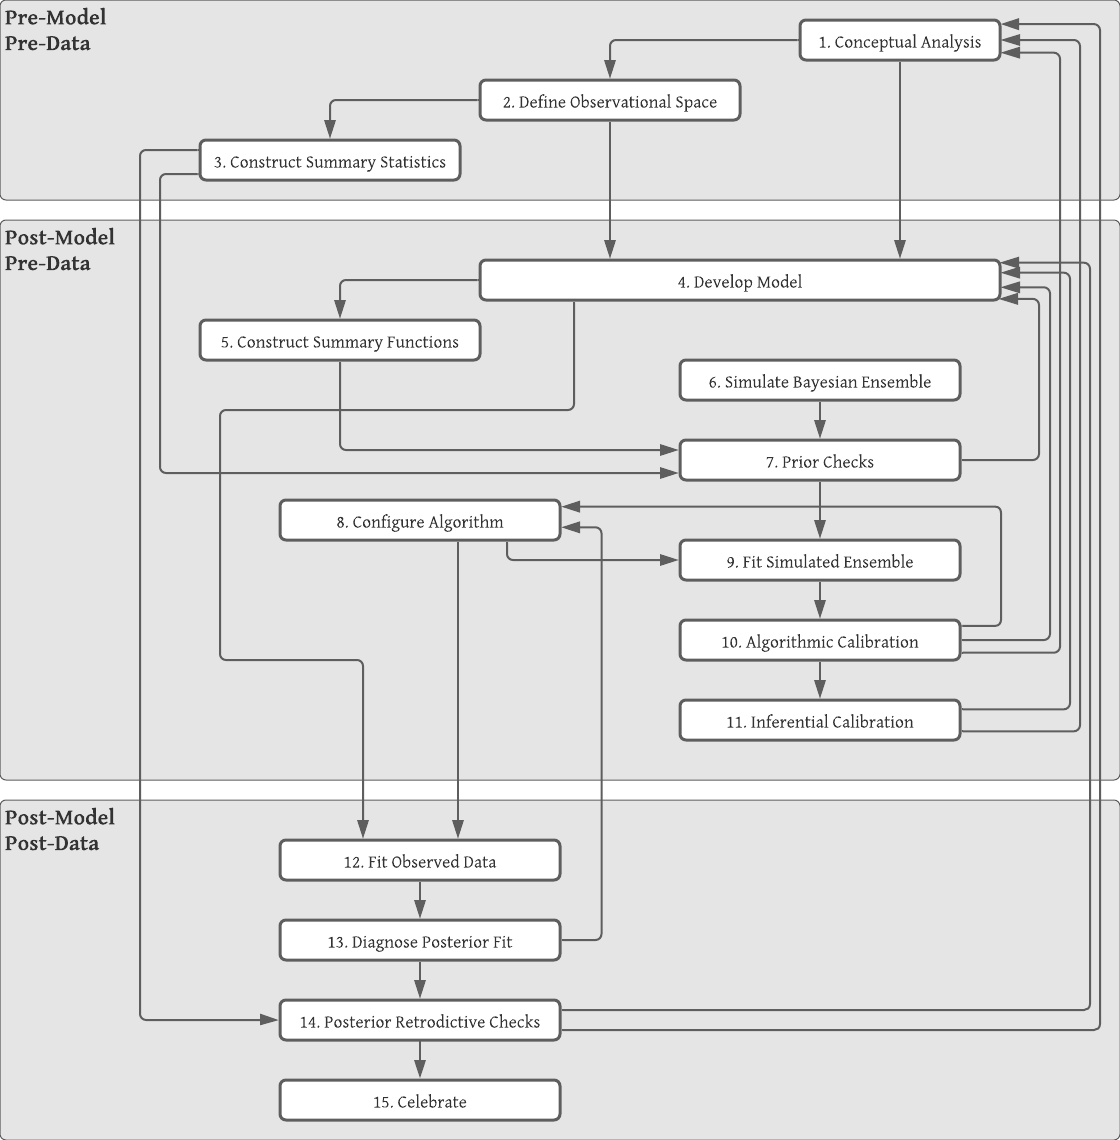
\includegraphics[width=1\linewidth]{figures/workflow-diagram} 

}

\caption{Diagram is copywrited material of Michael Betancourt and used under the CC BY-NC 4.0 license. Image created with Lucid app.}\label{fig:ch030-workflow-diagram}
\end{figure}

\hypertarget{data}{%
\chapter{Motivating data}\label{data}}

This paper focuses on a type of psychometric experiment called a temporal order judgment (TOJ) experiment. If there are two distinct stimuli occurring nearly simultaneously then our brains will bind them into a single percept (perceive them as happening simultaneously). Compensation for small temporal differences is beneficial for coherent multisensory experiences, particularly in visual-speech synthesis as it is necessary to maintain an accurate representation of the sources of multisensory events.

It was Charles Darwin who in his book ``On the Origin of Species'' developed the idea that living organisms adapt in order to better survive in their environment. Sir Francis Galton, inspired by Darwin's ideas, became interested in the differences in human beings and in how to measure those differences. Galton's works on studying and measuring human differences lead to the creation of psychometrics -- the science of measuring mental faculties. Around the same time that he was developing his theories, Johann Friedrich Herbart was also interested in studying consciousness through the scientific method, and is responsible for creating mathematical models of the mind.

E.H. Weber built upon Herbart's work, and sought out to prove the idea of a psychological threshold. A psychological threshold is a minimum stimulus intensity necessary to activate a sensory system -- a liminal stimulus. He paved the way for experimental psychology and is the namesake of Weber's Law (Equation \eqref{eq:webers-law}), which states that the change in a stimulus that will be just noticeable is a constant ratio of the original stimulus \citep{ekman1959weber}.

\begin{equation}
  \frac{\Delta I}{I} = k
  \label{eq:webers-law}
\end{equation}

To demonstrate this law, consider holding a 1 kg weight (\(I = 1\)), and further suppose that the difference between a 1 kg weight and a 1.2 kg weight (\(\Delta I = 0.2\)) can just be detected. Then the constant just noticeable ratio is:

\[k = \frac{0.2}{1} = 0.2\]

Now consider picking up a 10 kg weight. The mass required to just detect a difference can be calculated as:

\[\frac{\Delta I}{10} = 0.2 \Rightarrow \Delta I = 2\]

The difference between a 10 kg and a 12 kg weight is expected to be just barely perceptible. Note that the difference in the first set of weights is 0.2, and in the second set it is 2. The perception of the difference in stimulus intensities is not absolute, but relative. G.T. Fechner devised the law (Weber-Fechner Law, Equation \eqref{eq:weber-fechner-law}) that the strength of a sensation grows as the logarithm of the stimulus intensity.

\begin{equation}
  S = K \ln I
  \label{eq:weber-fechner-law}
\end{equation}

Consider two light sources: one that is 100 lumens (\(S_1 = K \ln 100\)) and another that is 200 lumens (\(S_2 = K \ln 200\)). The intensity of the second light is not perceived as twice as bright, but only about 1.15 times as bright according to \eqref{eq:weber-fechner-law}:

\[\theta = S_2 / S_1 \approx 1.15\]

Notice that the value \(K\) cancels out when calculating the relative intensity, but knowing \(K\) can lead to important psychological insights about differences between persons or groups of people. What biological and contextual factors affect how people perceive different stimuli? How do we measure their perception in a meaningful way? We can collect data from psychometric experiments, fit a model to the data from a family of functions called psychometric functions, and inspect key operating characteristics of those functions.

\hypertarget{psycho-experiments}{%
\section{Psychometric experiments}\label{psycho-experiments}}

Psychometric experiments are devised in a way to examine psychophysical processes, or the response between the world around us and our inward perceptions. A psychometric function relates an observer's performance to an independent variable, usually some physical quantity of a stimulus in a psychophysical task \citep{wichmann2001a}. Psychometric functions were studied as early as the late 1800's, and Edwin Boring published a chart of the psychometric function in The American Journal of Psychology in 1917 \citep{boring1917chart}.

\begin{figure}

{\centering 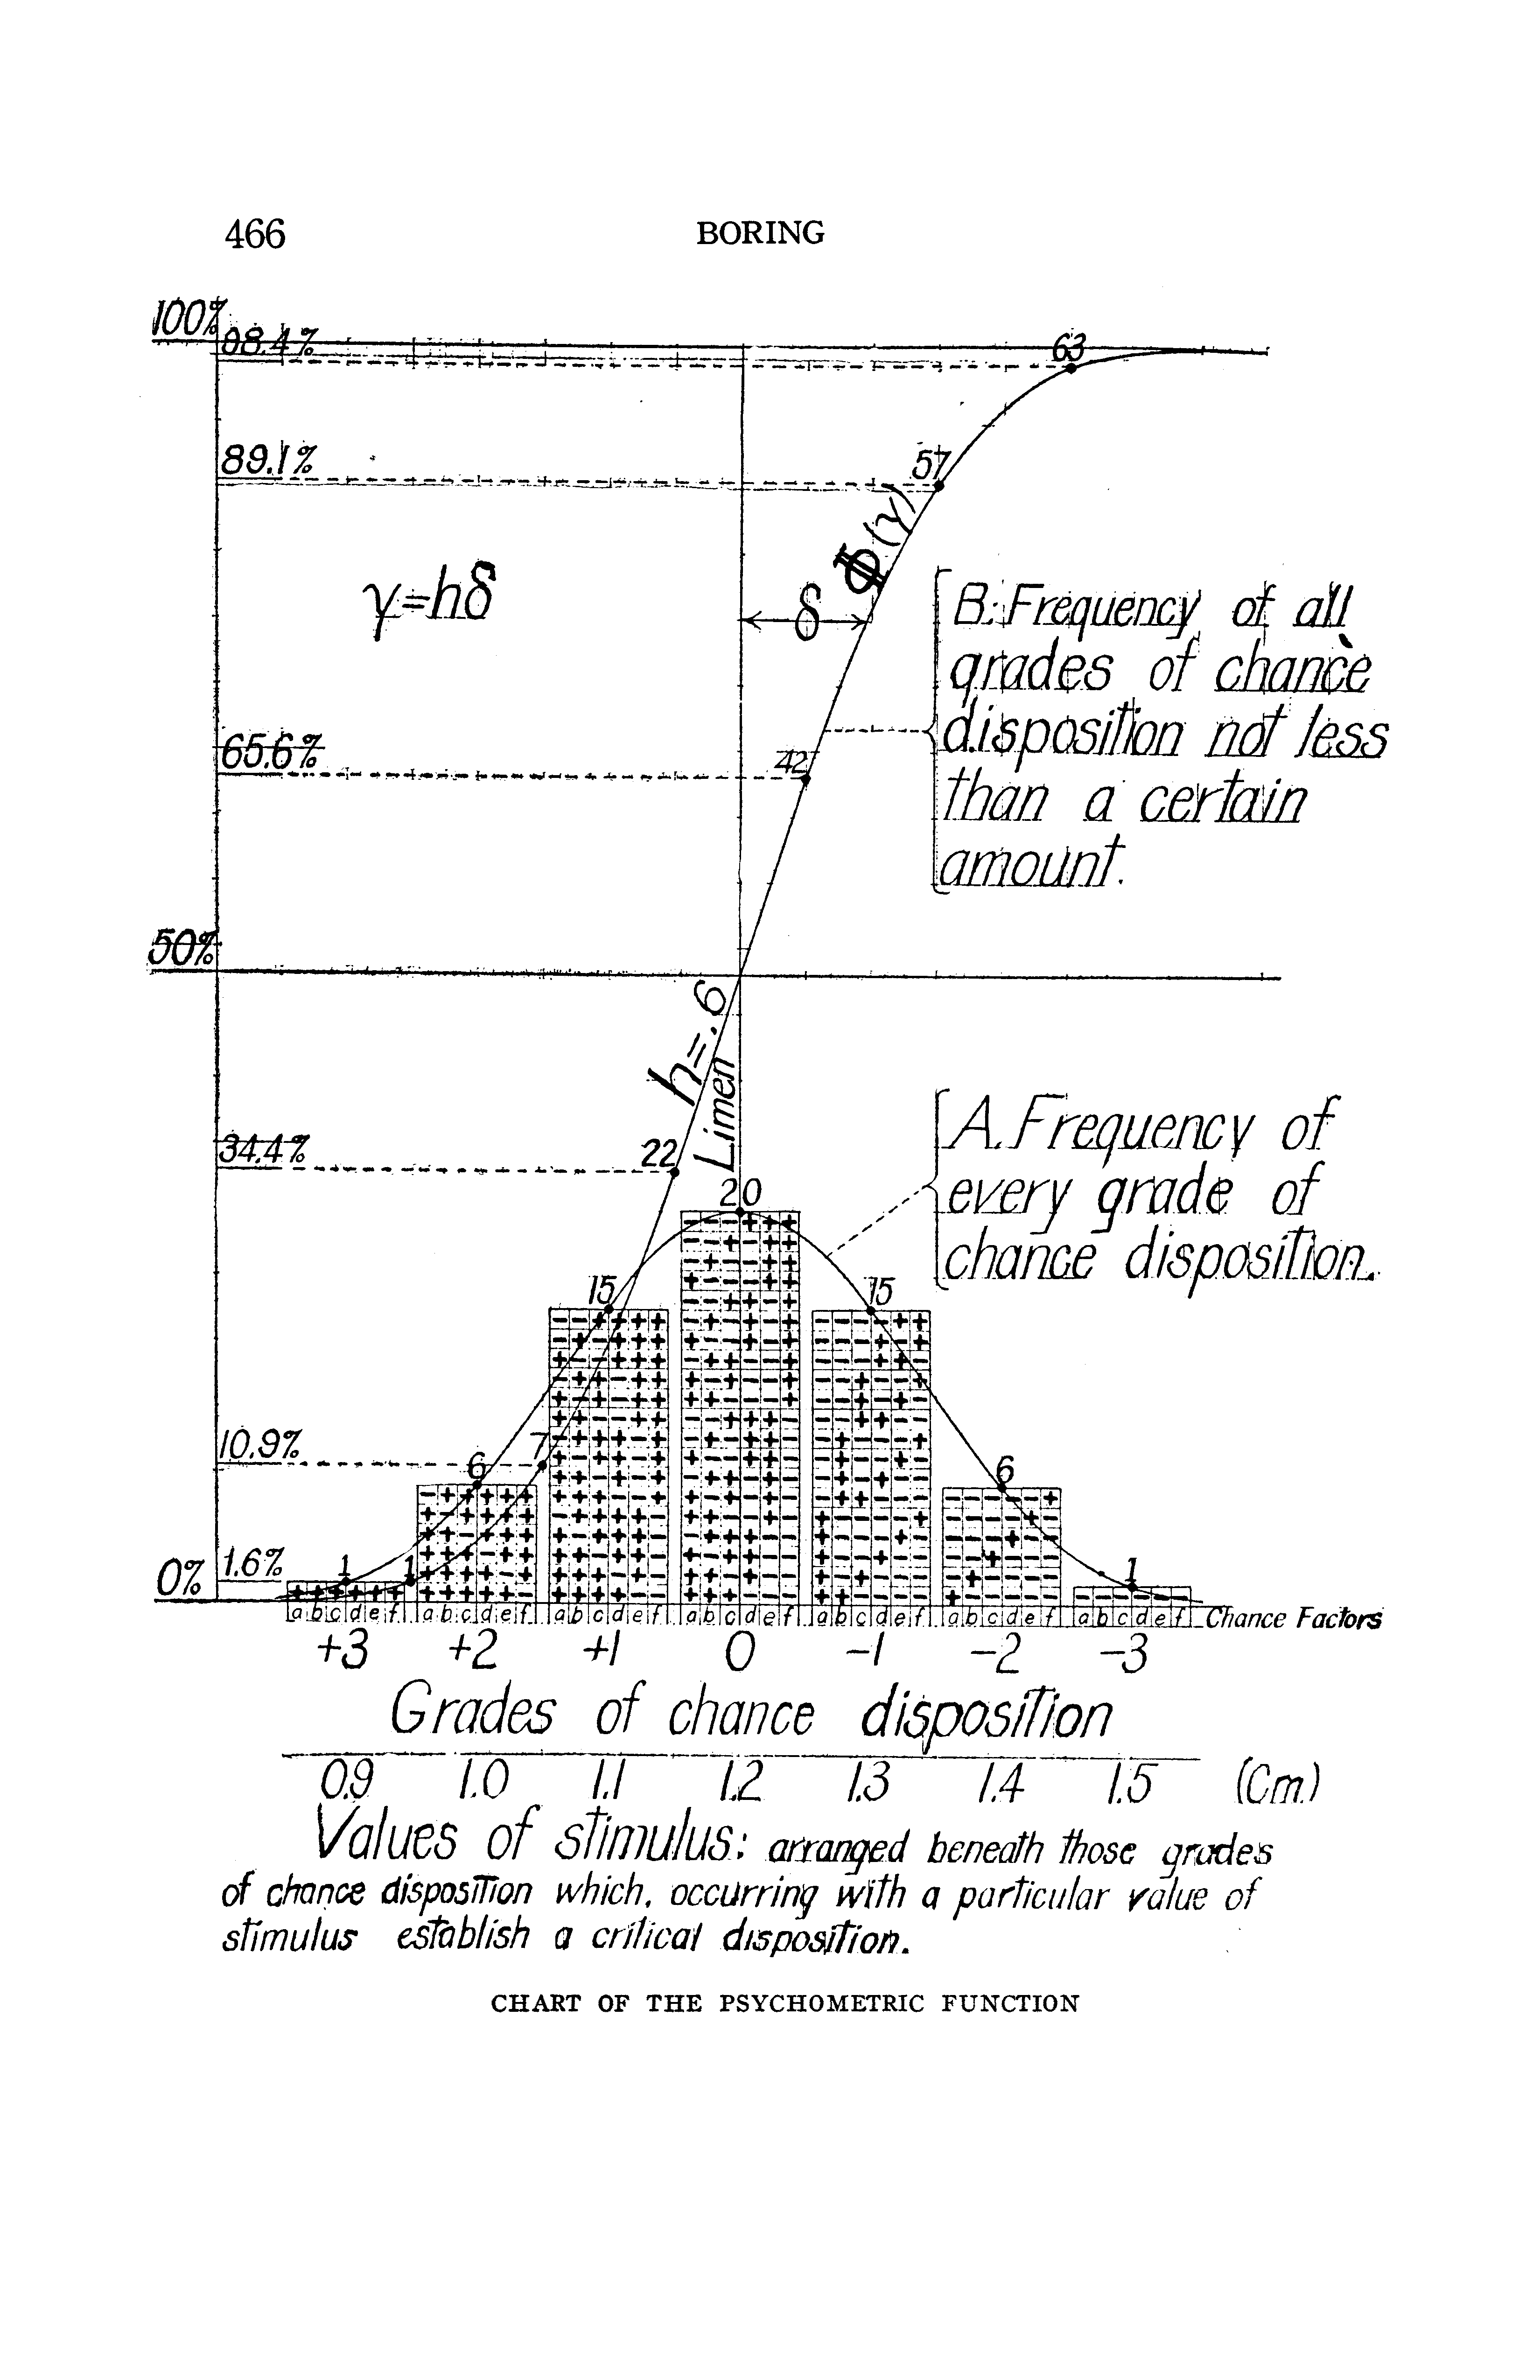
\includegraphics[width=0.85\linewidth]{figures/chart_of_pf} 

}

\caption{A chart of the psychometric function. The experiment in this paper places two points on a subject's skin separated by some distance, and has them answer their impression of whether there is one point or two, recorded as either `two points` or `not two points`. As the separation of aesthesiometer points increases, so too does the subject's confidence in their perception of `two-ness`. So at what separation is the impression of two points liminal?}\label{fig:ch020-chart-of-pf}
\end{figure}

Figure \ref{fig:ch020-chart-of-pf} displays the key aspects of the psychometric function. The most crucial part is the sigmoid function, the S-like non-decreasing curve which in this case is represented by the Normal CDF, \(\Phi(\gamma)\). The horizontal axis represents the stimulus intensity: the separation of two points in centimeters. The vertical axis represents the probability that a subject has the impression of two points. With only experimental data, the response proportion becomes an approximation for the probability.

The temporal asynchrony between stimuli is called the stimulus onset asynchrony (SOA), and the range of SOAs for which sensory signals are integrated into a global percept is called the temporal binding window. When the SOA grows large enough, the brain segregates the two signals and the temporal order can be determined.

Our experiences in life as we age shape the mechanisms of processing multisensory signals, and some multisensory signals are integrated much more readily than others. Perceptual synchrony has been previously studied through the point of subjective simultaneity (PSS) -- the temporal delay between two signals at which an observer is unsure about their temporal order \citep{stone2001now}. The temporal binding window is the time span over which sensory signals arising from different modalities appear integrated into a global percept.

A deficit in temporal sensitivity may lead to a widening of the temporal binding window and reduce the ability to segregate unrelated sensory signals. In TOJ tasks, the ability to discriminate the timing of multiple sensory signals is referred to as temporal sensitivity, and is studied through the measurement of the just noticeable difference (JND) -- the smallest lapse in time so that a temporal order can just be determined.

Figure \ref{fig:ch020-plot-ref-pf} highlights the features through which we study psychometric functions. The PSS is defined as the point where an observer can do no better at determining temporal order than random guessing (i.e.~when the response probability is 50\%). The JND is defined as the extra temporal delay between stimuli so that the temporal order is just able to be determined. Historically this has been defined as the difference between the 84\% level -- one standard deviation away from the mean -- and the PSS, though the upper level often depends on domain expertise.

\begin{figure}

{\centering 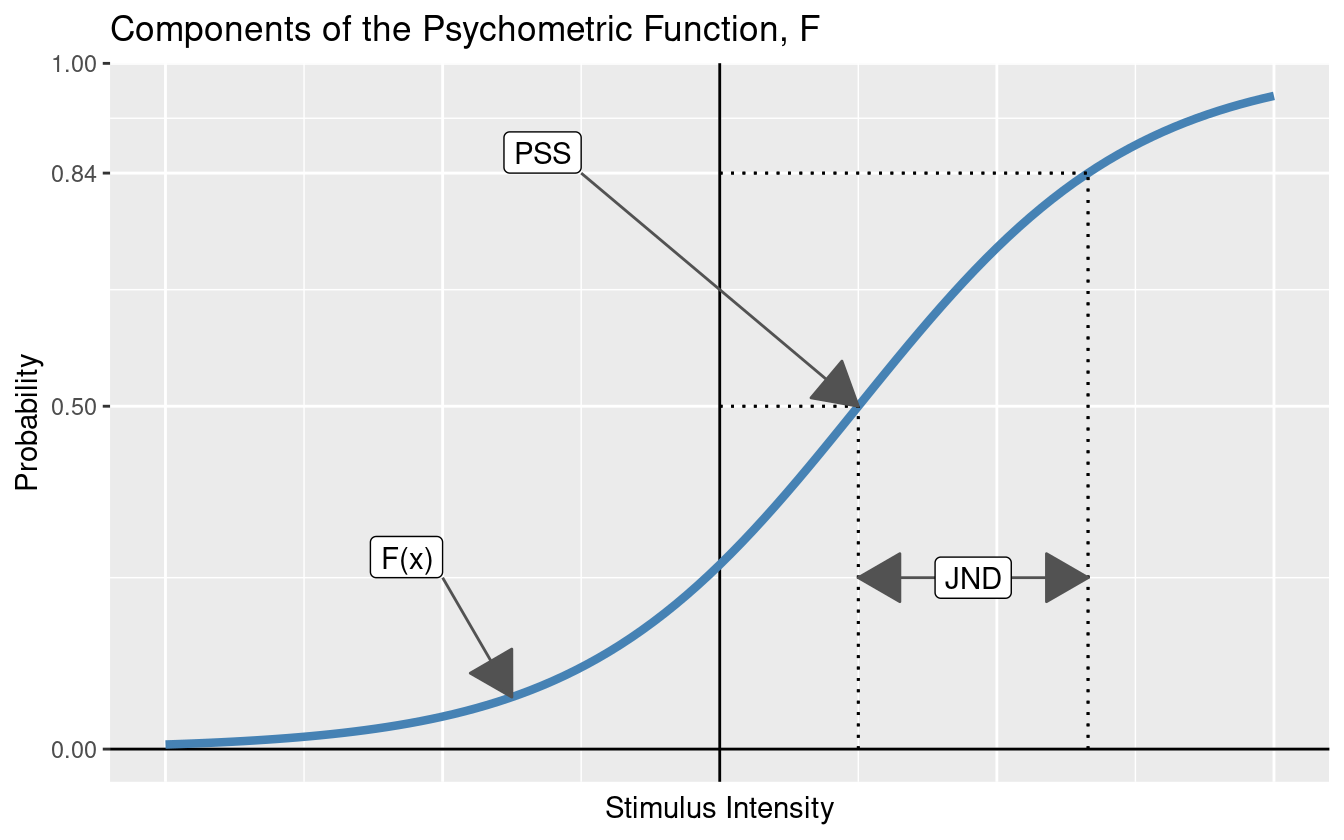
\includegraphics[width=0.85\linewidth]{020-psychometrics_files/figure-latex/ch020-plot-ref-pf-1} 

}

\caption{The PSS is defined as the point where an observer can do no better at determining temporal order than random guessing. The just noticeable difference is defined as the extra temporal delay between stimuli so that the temporal order is just able to be determined. Historically this has been defined as the difference between the 0.84 level and the PSS, though the upper level depends on domain expertise.}\label{fig:ch020-plot-ref-pf}
\end{figure}

\hypertarget{toj-task}{%
\section{Temporal order judgment tasks}\label{toj-task}}

The data set used in this paper comes from small-scale preliminary experiments done by A.N. Scurry and Dr.~Jiang in the Department of Psychology at the University of Nevada. Reduced temporal sensitivity in the aging population manifests in an impaired ability to perceive synchronous events as simultaneous, and similarly more difficulty in segregating asynchronous sensory signals that belong to different sources. The consequences of a widening of the temporal binding window is considered in \citet{scurry2019aging}, as well as a complete detailing of the experimental setup and recording process. Here we present a shortened summary of the experimental methods.

There are four different tasks in the experiment: audio-visual, visual-visual, visual-motor, and duration, and each task is respectively referred to as audiovisual, visual, sensorimotor, and duration. The participants consist of 15 young adults (age 20-27), 15 middle age adults (age 39-50), and 15 older adults (age 65-75), all recruited from the University of Nevada, Reno. Additionally all subjects are right handed and are reported to have normal or corrected to normal hearing and vision.

\begin{table}[!h]

\caption{\label{tab:ch020-multitask-data}Sample of motivating data.}
\centering
\begin{tabular}[t]{rrllllrl}
\toprule
soa & response & sid & task & block & age\_group & age & sex\\
\midrule
-350 & 0 & O-m-BC & audiovisual & baseline & older & 70 & M\\
200 & 1 & M-f-TW & visual & adapt1 & middle & 49 & F\\
28 & 1 & O-f-KK & sensorimotor & baseline & older & 66 & F\\
150 & 1 & Y-m-CB & duration & adapt1 & young & 22 & M\\
\bottomrule
\end{tabular}
\end{table}

In the audiovisual TOJ task, participants were asked to determine the temporal order between an auditory and visual stimulus. Stimulus onset asynchrony values were selected uniformly between -500 to +500 ms with 50 ms steps, where negative SOAs indicated that the visual stimulus was leading, and positive values indicated that the auditory stimulus was leading. Each SOA value was presented 5 times in random order in the initial block. At the end of each trial the subject was asked to report if the auditory stimulus came before the visual, where a \(1\) indicates that they perceived the sound first, and a \(0\) indicates that they perceived the visual stimulus first.

A similar setup is repeated for the visual, sensorimotor, and duration tasks. The visual task presented two visual stimuli on the left and right side of a display with temporal asynchronies that varied between -300 ms to +300 ms with 25 ms steps. Negative SOAs indicated that the left stimulus was first, and positive that the right came first. A positive response indicates that the subject perceived the right stimulus first.

The sensorimotor task has subjects focus on a black cross on a screen. When it disappears, they respond by pressing a button. Additionally, when the cross disappears, a visual stimulus was flashed on the screen, and subjects were asked if they perceived the visual stimulus before or after their button press. The latency of the visual stimulus was partially determined by individual subject's average response time, so SOA values are not fixed between subjects and trials. A positive response indicates that the visual stimulus was perceived after the button press.

The duration task presents two vertically stacked circles on a screen with one appearing right after the other. The top stimulus appeared for a fixed amount of time of 300 ms, and the bottom was displayed for anywhere between +100 ms to +500 ms in 50 ms steps corresponding to SOA values between -200 ms to +200 ms. The subject then responds to if they perceived the bottom circle as appearing longer than the top circle.

\begin{table}[!h]

\caption{\label{tab:ch020-toj-summary}Summary of TOJ Tasks}
\centering
\begin{tabular}[t]{lll}
\toprule
Task & Positive Response & Positive SOA Truth\\
\midrule
Audiovisual & Perceived audio first & Audio came before visual\\
Visual & Perceived right first & Right came before left\\
Sensorimotor & Perceived visual first & Visual came before tactile\\
Duration & Perceived bottom as longer & Bottom lasted longer than top\\
\bottomrule
\end{tabular}
\end{table}

Perceptual synchrony and temporal sensitivity can be modified through a baseline understanding. In order to perceive physical events as simultaneous, our brains must adjust for differences in temporal delays of transmission of both psychical signals and sensory processing \citep{fujisaki2004recalibration}. In some cases such as with audiovisual stimuli, the perception of simultaneity can be modified by repeatedly presenting the audiovisual stimuli at fixed time separations (called an adapter stimulus) to an observer \citep{vroomen2004recalibration}. This repetition of presenting the adapter stimulus is called temporal recalibration.

After the first block of each task was completed, the participants went through an adaptation period where they were presented with the respective stimuli from each task repeatedly at fixed temporal delays, then the TOJ task was repeated. To ensure that the adaptation affect persisted, the subject was presented with the adapter stimulus at regular intervals throughout the second block. The blocks are designated as \texttt{pre} and \texttt{post1}, \texttt{post2}, etc. in the data set. In this paper we only focus on the baseline block (\texttt{pre}) and the post-adaptation block (\texttt{post1}).

\hypertarget{data-visualization-and-quirks}{%
\section{Data visualization and quirks}\label{data-visualization-and-quirks}}

The dependent variable in these TOJ experiments is the subject's perceived response, encoded as a 0 or a 1, and the independent variable is the SOA value. If the response is plotted against the SOA values, then it is difficult to determine the relationship (see the right panel of figure \ref{fig:ch020-simple-response-soa-plot}). Transparency can be used to better visualize the relationship. The center panel in figure \ref{fig:ch020-simple-response-soa-plot} shows the same data as the left, except that the transparency is set to \(0.05\). Note that there is a higher density of ``0'' responses towards more negative SOAs, and a higher density of ``1'' responses for more positive SOAs. The proportion of ``positive'' responses for a given SOA is computed and plotted against the SOA value (displayed in the right panel of figure \ref{fig:ch020-simple-response-soa-plot}). The relationship between SOA values and responses is clear -- as the SOA value goes from more negative to more positive, the proportion of positive responses increases from near 0 to near 1.

\begin{figure}

{\centering 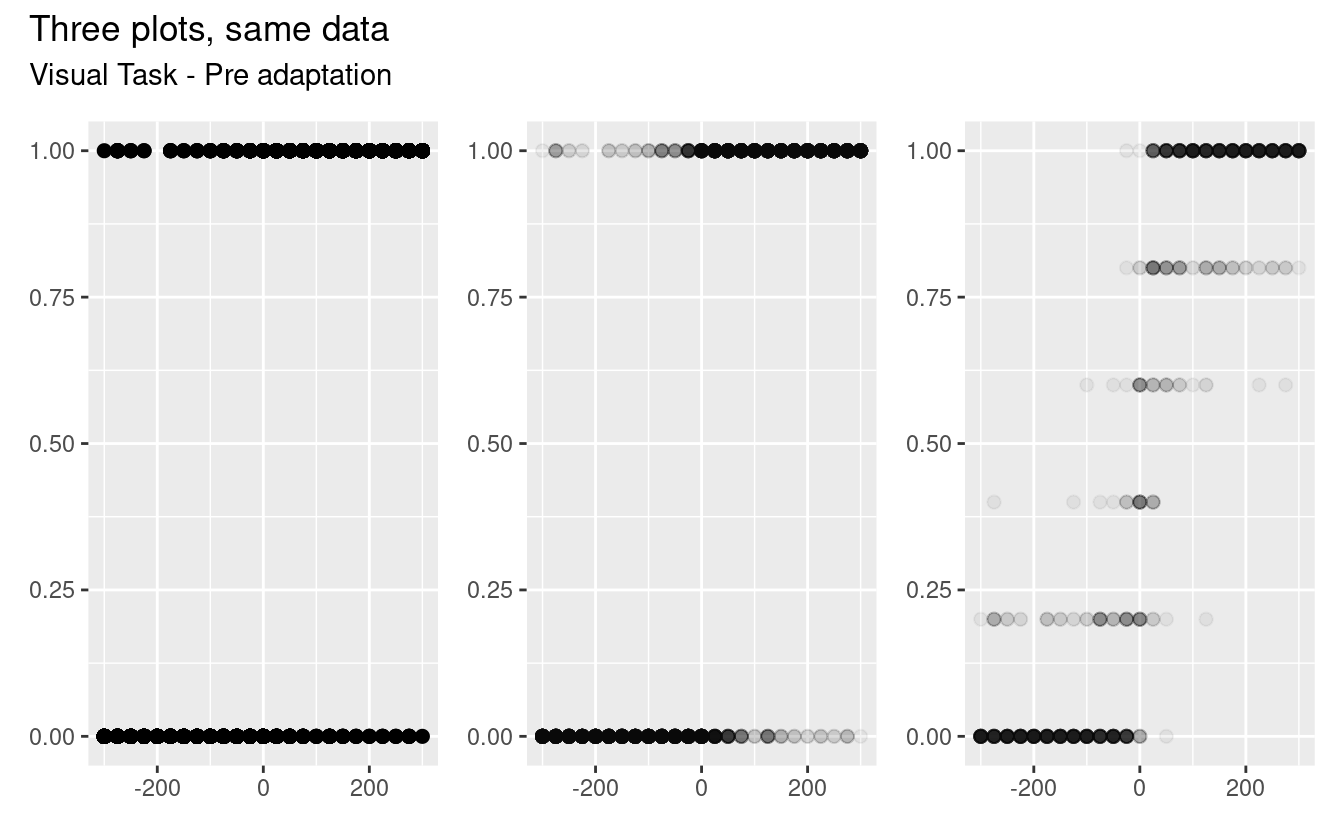
\includegraphics[width=0.85\linewidth]{020-psychometrics_files/figure-latex/ch020-simple-response-soa-plot-1} 

}

\caption{Left: Simple plot of response vs. soa value. Center: A plot of response vs. soa with transparency. Right: A plot of proportions vs. soa with transparency.}\label{fig:ch020-simple-response-soa-plot}
\end{figure}

The right panel in figure \ref{fig:ch020-simple-response-soa-plot} is the easiest to interpret, and we often present the observed and predicted data using the proportion of responses rather than the raw responses. Proportional data is also bounded on the same interval as the response in contrast to the raw counts.

For the audiovisual task, the responses can be aggregated into binomial data -- the number of positive responses for given SOA value -- which is more efficient to work with than the Bernoulli data (see table \ref{tab:ch020-av-bin-sample}). However the number of times an SOA is presented varies between the pre-adaptation and post-adaptation blocks; 5 and 3 times per SOA respectively.

\begin{table}[!h]

\caption{\label{tab:ch020-av-bin-sample}Audiovisual task with aggregated responses.}
\centering
\begin{tabular}[t]{lrrrr}
\toprule
block & soa & n & k & proportion\\
\midrule
 & 200 & 5 & 4 & 0.80\\
\cmidrule{2-5}
 & 150 & 5 & 5 & 1.00\\
\cmidrule{2-5}
\multirow[t]{-3}{*}{\raggedright\arraybackslash baseline} & -350 & 5 & 0 & 0.00\\
\cmidrule{1-5}
 & 350 & 3 & 3 & 1.00\\
\cmidrule{2-5}
 & -500 & 3 & 1 & 0.33\\
\cmidrule{2-5}
\multirow[t]{-3}{*}{\raggedright\arraybackslash adapt1} & -200 & 3 & 0 & 0.00\\
\bottomrule
\end{tabular}
\end{table}

There is one younger subject that did not complete the audiovisual task, and one younger subject that did not complete the duration task. There is also one older subject who's response data for the post-adaptation audiovisual task is unreasonable -- it is extremely unlikely that the data represents genuine responses (see figure \ref{fig:ch020-av-post1-O-f-CE-plot}).

\begin{figure}

{\centering 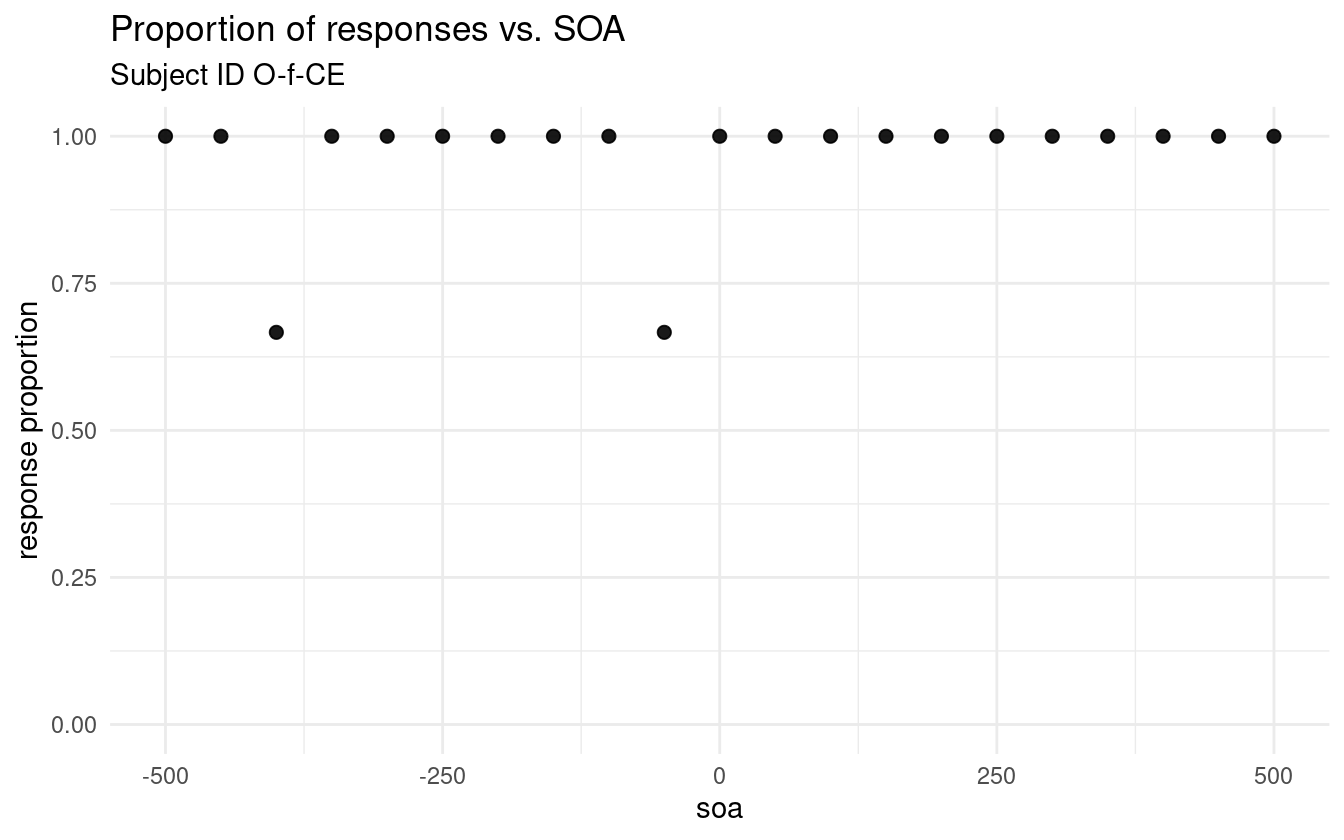
\includegraphics[width=0.85\linewidth]{020-psychometrics_files/figure-latex/ch020-av-post1-O-f-CE-plot-1} 

}

\caption{Post-adaptation response data for O-f-CE}\label{fig:ch020-av-post1-O-f-CE-plot}
\end{figure}

Of all the negative SOAs, there were only two ``correct'' responses (the perceived order matches the actual order). If a subject is randomly guessing the temporal order, then a naive estimate for the proportion of correct responses is 0.5. If a subject's proportion of correct responses is above 0.5, then they are doing better than random guessing. Figure \ref{fig:ch020-av-post-neg-trials} shows that subject \texttt{O-f-CE} is the only one who's proportion is below 0.5 (and by a considerable amount), and so their post-adaptation block is removed from data set for model fitting.

\begin{figure}

{\centering 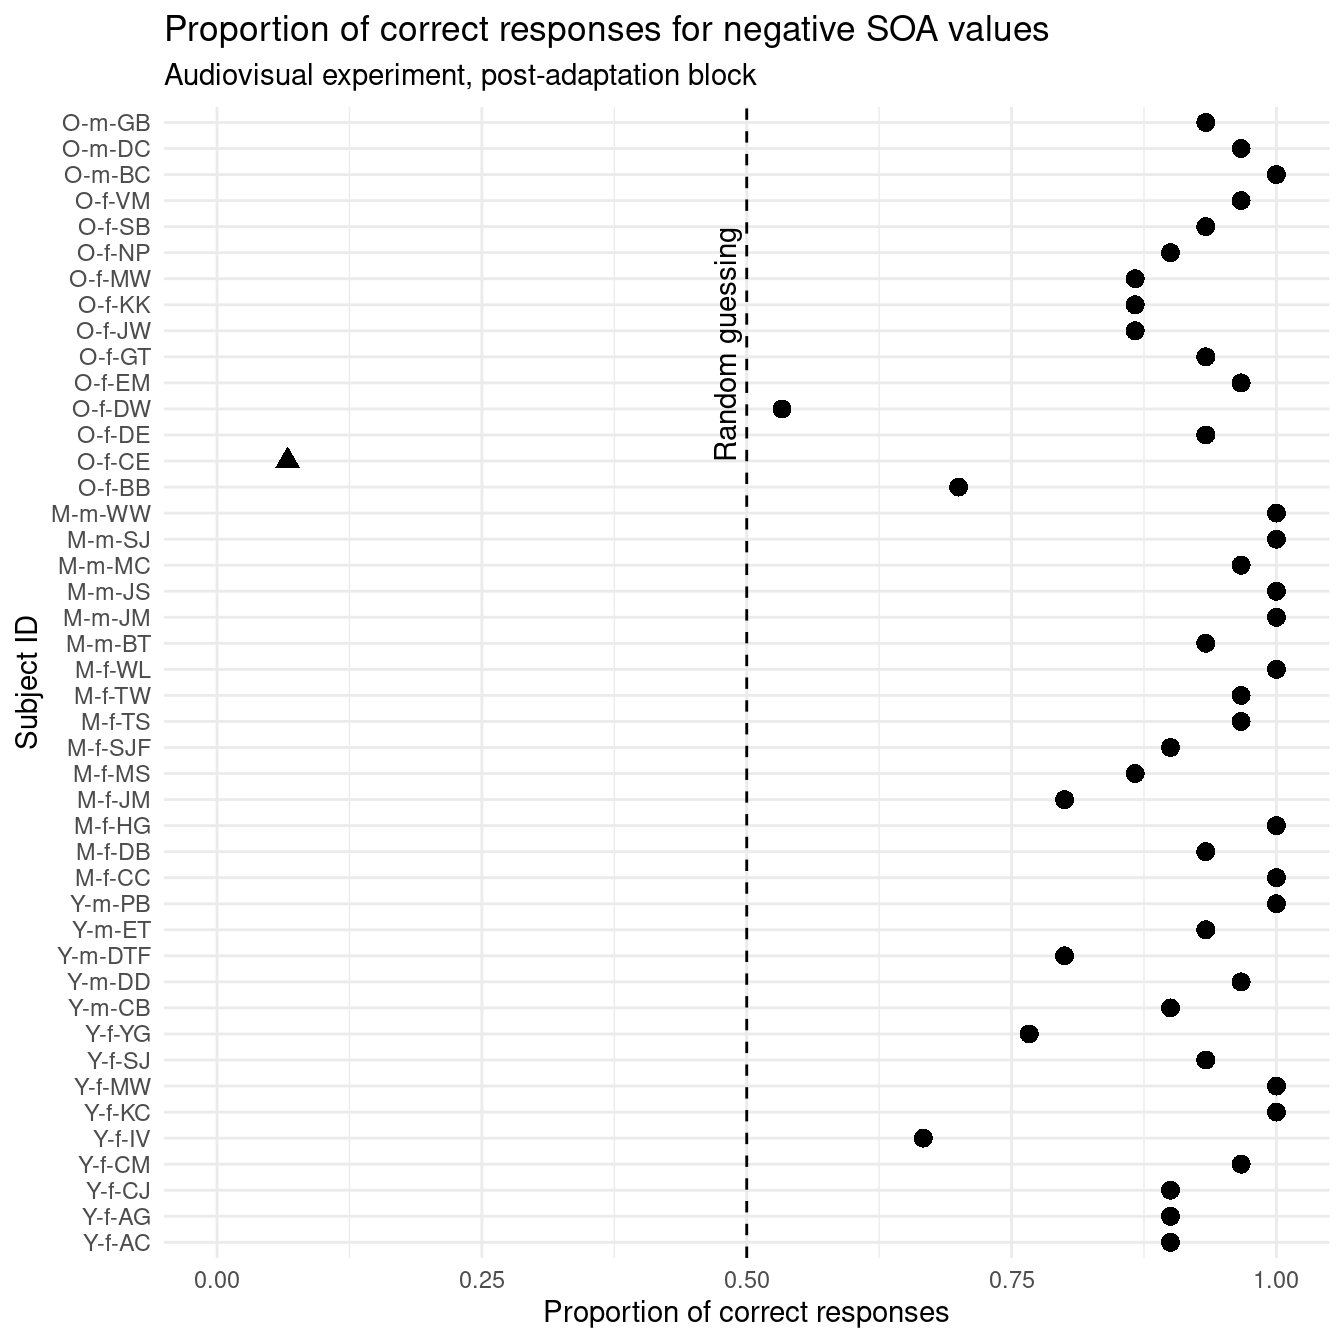
\includegraphics[width=0.85\linewidth]{020-psychometrics_files/figure-latex/ch020-av-post-neg-trials-1} 

}

\caption{Proportion of correct responses for negative SOA values during the post-adaptation audiovisual experiment.}\label{fig:ch020-av-post-neg-trials}
\end{figure}

\hypertarget{application}{%
\chapter{Bayesian Multilevel Modeling of the Psychometric Function}\label{application}}

Now we apply the workflow to our data set, seeking to build a model that satisfies the four criteria in \protect\hyperlink{methods}{chapter 2}. During model refinement, we'll pick up on the regular features while assessing the statistical significance of covariates through predictive comparison. In our final model, we'll model well-known data quality issues (from participant lapses in judgment) and show that this improves model prediction.

As we iterate through our model development workflow, we have a preference for multilevel models (for the reasons discussed in \protect\hyperlink{methods}{chapter 2}). Hierarchical models are a specific kind of multilevel model where one or more groups are nested within a larger one. In the case of the psychometric data, there are three age groups, and within each age group are individual subjects.

\hypertarget{psych-quant}{%
\section{Modeling psychometric quantities}\label{psych-quant}}

Before formally conducting the workflow, we motivate our choice of using the logistic function to model the psychometric function as well as our choice for the parameterization of the linear predictor. Three common sigmoid functions are displayed in figure \ref{fig:ch040-pf-assortment}.

\begin{figure}

{\centering 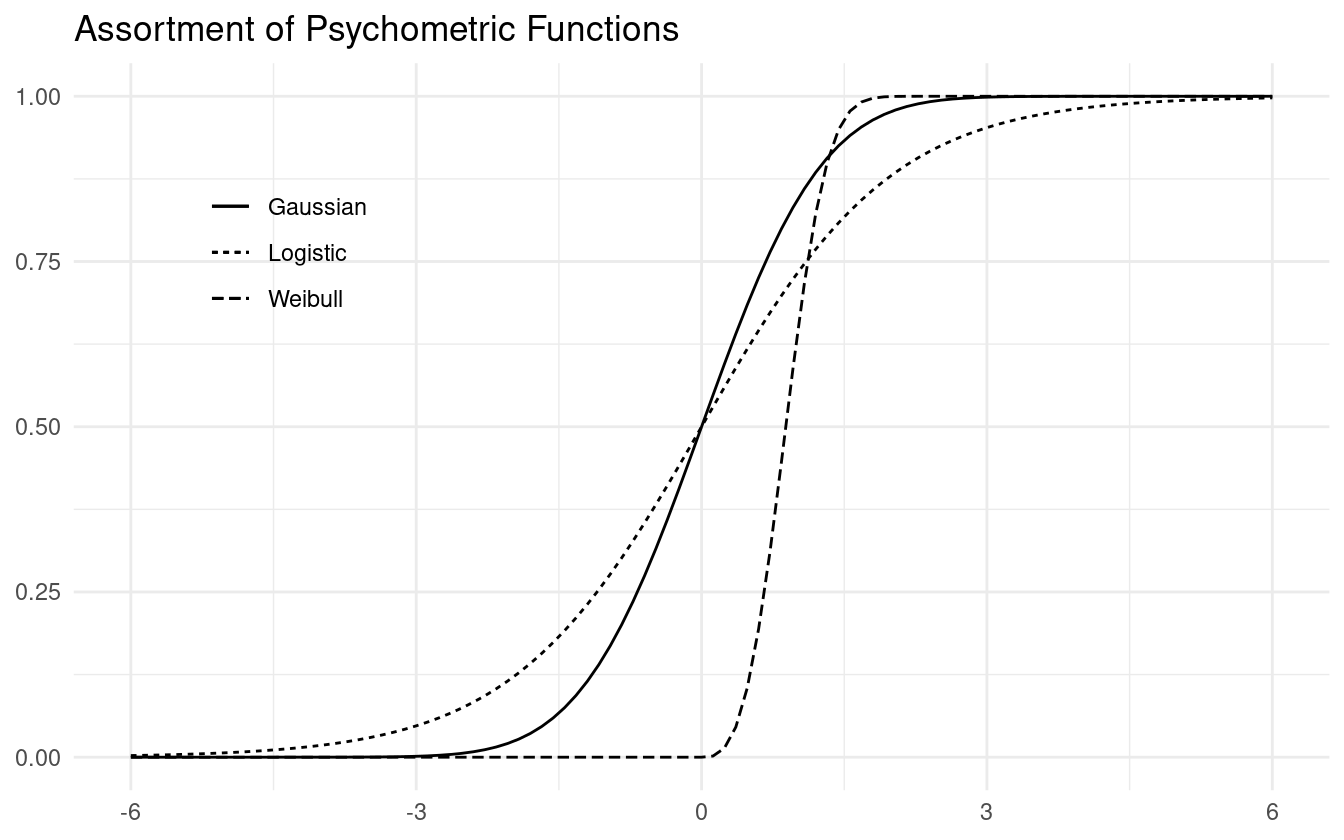
\includegraphics[width=0.85\linewidth]{040-application_files/figure-latex/ch040-pf-assortment-1} 

}

\caption{Assortment of psychometric functions.}\label{fig:ch040-pf-assortment}
\end{figure}

The Weibull psychometric function is more common when it comes to 2-alternative forced choice (2-AFC) psychometric experiments where the independent variable is a stimulus intensity (non-negative) and the goal is signal detection. The data in this paper includes both positive and negative SOA values, so the Weibull is not a natural choice. Our first choice is the logistic function as it is the canonical choice for Binomial count data. The data in this study are exchangeable, meaning that the label of a positive response can be swapped with the label of a negative response and the inferences would remain the same. Since there is no natural ordering, it makes more sense for the psychometric function to be symmetric, e.g.~the logistic function and Gaussian CDF. We use symmetric loosely to mean that the probability density function (PDF) has zero skewness. In practice, there is little difference in inferences between the logit and probit links, but computationally the logit link is more efficient.

It is appropriate to provide additional background to GLMs and their role in working with psychometric functions. A GLM allows the linear model to be related to the outcome variable via a link function. An example of this is the logit link -- the inverse of the logistic function. The logistic function, \(F\), takes \(x \in \mathbb{R}\) and constrains the output to be in \((0, 1)\).

\begin{equation}
  F(\theta) = \frac{1}{1 + \exp\left(-\theta\right)}
  \label{eq:logistic}
\end{equation}

Since \(F\) is a strictly increasing and continuous function, it has an inverse, and the link for \eqref{eq:logistic} is the log-odds or logit function.

\begin{equation}
  F^{-1}(\pi) = \mathrm{logit}(\pi) = \ln\left(\frac{\pi}{1 - \pi}\right)
  \label{eq:logit}
\end{equation}

By taking \((F^{-1} \circ F)(\theta)\) we can arrive at a relationship that is linear in \(\theta\).

\setstretch{1.0}

\begin{align*}
  \pi = F(\theta) \Longleftrightarrow F^{-1}(\pi) &= F^{-1}(F(\theta)) \\
  & = \ln\left(\frac{F(\theta)}{1 - F(\theta)}\right) \\
  &= \ln(F(\theta)) - \ln(1 - F(\theta)) \\
  &= \ln\left(\frac{1}{1 + \exp(-\theta)}\right) - \ln\left(\frac{\exp(-\theta)}{1 + \exp(-\theta)}\right) \\
  &= - \ln(1 + \exp(-\theta)) - \ln(\exp(-\theta)) + \ln(1 + \exp(-\theta)) \\
  &= - \ln(\exp(-\theta)) \\
  &= \theta
\end{align*}
\setstretch{2.0}

The motivation for this background is to show that a model for the psychometric function can be specified using a linear predictor, \(\theta\). Given a simple slope-intercept model, the linear predictor would typically be written as:

\begin{equation}
  \theta = \alpha + \beta x
  \label{eq:linearform1}
\end{equation}

This isn't the only possible form; it could be written in the slope-location parameterization:

\begin{equation}
  \theta = \beta(x - a)
  \label{eq:linearform2}
\end{equation}

Both parameterizations will describe the same geometry, so why should it matter which form is chosen? The interpretation of the parameters change between the two models, but the reason becomes clear when we consider how the linear model relates back to the physical properties that the psychometric model describes. Take equation \eqref{eq:linearform1}, substitute it in to \eqref{eq:logistic}, and then take the logit of both sides:

\begin{equation}
  \mathrm{logit}(\pi) = \alpha+\beta x
  \label{eq:pfform1}
\end{equation}

Now recall that the PSS is defined as the SOA value such that the response probability, \(\pi\), is \(0.5\). Substituting \(\pi = 0.5\) into \eqref{eq:pfform1} and solving for \(x\) yields:

\[pss = -\frac{\alpha}{\beta}\]

Similarly, the JND is defined as the difference between the SOA value at the 84\% level and the PSS. Substituting \(\pi = 0.84\) into \eqref{eq:pfform1}, solving for \(x\), and subtracting off the pss yields:

\begin{equation}
  jnd = \frac{\mathrm{logit}(0.84)}{\beta}
  \label{eq:jnd1}
\end{equation}

From the conceptual analysis, it is easy to define priors for the PSS and JND, but then how does one set the priors for \(\alpha\) and \(\beta\)? Let's say the prior for the just noticeable difference is \(jnd \sim \pi_j\). Then the prior for \(\beta\) would be:

\[\beta \sim \frac{\mathrm{logit}(0.84)}{\pi_j}\]

The log-normal distribution has a nice property where its multiplicative inverse is still a log-normal distribution. If we let \(\pi_j = \mathrm{Lognormal}(\mu, \sigma^2)\), then \(\beta\) would be distributed as:

\[
\beta \sim \mathrm{Lognormal}(-\mu + \ln(\mathrm{logit}(0.84)), \sigma^2)
\]

This is acceptable as the slope must always be positive for this psychometric data, and a log-normal distribution constrains the support to positive real numbers. Next suppose that the prior distribution for the PSS is \(pss \sim \pi_p\). Then the prior for \(\alpha\) is:

\[\alpha \sim -\pi_p \cdot \beta\]

If \(\pi_p\) is set to a log-normal distribution as well, then \(\pi_p \cdot \beta\) would also be log-normal, but there is still the problem of the negative sign. If \(\alpha\) is always negative, then the PSS will also always be negative, which is certainly not always true. Furthermore, we don't want to \emph{a priori} put more weight on positive PSS values compared to negative ones.

Let's now consider using equation \eqref{eq:linearform2} and repeat the above process.

\begin{equation}
  \mathrm{logit}(\pi) = \beta(x - a)
  \label{eq:pfform2}
\end{equation}

The just noticeable difference is still given by \eqref{eq:jnd1}, and so the same method for choosing a prior can be used. However, the PSS is now given by:

\[pss = \alpha\]

This is a fortunate consequence of using \eqref{eq:linearform2} because now the JND only depends on \(\beta\) and the PSS only depends on \(\alpha\). Additionally \(\alpha\) can be interpreted as the PSS of the estimated psychometric function. Also thrown in is the ability to set a prior for \(\alpha\) that is symmetric around \(0\) such as a Gaussian distribution.

This also highlights the benefit of using a modeling language like \texttt{Stan} over others. For fitting GLMs in \texttt{R}, one can use \texttt{stats::glm} which utilizes MLE, or others such as \texttt{rstanarm::stan\_glm} and \texttt{arm::bayesglm} that use Bayesian methods \citep{R-rstanarm, R-arm}. Each of these functions requires the linear predictor to be in the form of \eqref{eq:linearform1}. The \texttt{stan\_glm} function uses Stan in the back-end to fit a model, but is limited to priors from the Student-t family of distributions. By writing the model directly in \texttt{Stan}, the linear model can be parameterized in any way and with any prior distribution, and so allows for much more expressive modeling.

With the consideration for the choice of sigmoid function and linear parameterization complete, we begin to develop a multilevel model for the psychometric function.

\hypertarget{iter1}{%
\section{Iteration 1: base model}\label{iter1}}

\textbf{Pre-Model, Pre-Data}

\emph{Conceptual Analysis}

In section \ref{toj-task} we discussed the experimental setup and data collection. Subjects are presented with two stimuli separated by some temporal delay, and they are asked to respond as to their perception of the temporal order. There are 45 subjects with 15 each in the young, middle, and older age groups. As the SOA becomes larger in the positive direction, subjects are expected to give more ``positive'' responses, and as the SOA becomes larger in the negative direction, more ``negative'' responses are expected. By the way the experiment and responses are constructed, there is no expectation to see a reversal of this trend unless there was an issue with the subject's understanding of the directions given to them or an error in the recording process.

After the first experimental block the subjects go through a temporal recalibration period, and repeat the experiment. The interest is in seeing if the recalibration has an effect on temporal sensitivity and perceptual synchrony, and if the effect is different for each age group.

\emph{Define Observational Space}

The response that subjects give during a TOJ task is recorded as a zero or a one, and their relative performance is determined by the SOA value. Let \(y\) represent the binary outcome of a trial and let \(x\) be the SOA value.

\setstretch{1.0}

\begin{align*}
y_i &\in \lbrace 0, 1\rbrace \\
x_i &\in \mathbb{R}
\end{align*}
\setstretch{2.0}

If the SOA values are fixed as in the audiovisual task, then the responses can be aggregated into Binomial counts, \(k\).

\[k_i, n_i \in \mathbb{Z}_0^+, k_i \le n_i\]

In the above expression, \(\mathbb{Z}_0^+\) represents the set of non-negative integers. Notice that the number of trials \(n\) has an index variable \(i\). This is because the number of trials per SOA is not fixed between blocks. In the pre-adaptation block, there are five trials per SOA compared to three in the post-adaptation block. So if observation \(32\) is recorded during a ``pre'' block, \(n_{32} = 5\), and if observation \(1156\) is during a ``post'' block, \(n_{1156} = 3\).

Then there are three categorical variables: age group, subject ID, and trial (block). The first two are treated as factor variables (also known as index variable or categorical variable). Rather than using one-hot encoding or dummy variables, the age levels are left as categories, and a coefficient is fit for each level. If dummy variables were used for all 45 subjects, there would be 44 dummy variables to work with times the number of coefficients that make estimates at the subject level. The number of parameters in the model grows rapidly as the model complexity grows.

Age groups and individual subjects can be indexed in the same way that the number of trials is indexed. \(S_i\) refers to the subject in record \(i\), and similarly \(G_i\) refers to the age group of that subject. Observation \(63\) is for record ID av-adapt1-M-f-HG, so then \(S_{63}\) is M-f-HG and \(G_{63}\) is middle. Under the hood of \texttt{R}, these factor levels are represented as integers (e.g.~middle age group level is stored internally as the number 2).

\setstretch{1.0}

\begin{Shaded}
\begin{Highlighting}[]
\NormalTok{(x }\OtherTok{\textless{}{-}} \FunctionTok{factor}\NormalTok{(}\FunctionTok{c}\NormalTok{(}\StringTok{"a"}\NormalTok{, }\StringTok{"a"}\NormalTok{, }\StringTok{"b"}\NormalTok{, }\StringTok{"c"}\NormalTok{)))}
\CommentTok{\#\textgreater{} [1] a a b c}
\CommentTok{\#\textgreater{} Levels: a b c}
\FunctionTok{storage.mode}\NormalTok{(x)}
\CommentTok{\#\textgreater{} [1] "integer"}
\end{Highlighting}
\end{Shaded}

\setstretch{2.0}

This data storage representation can later be exploited for the \texttt{Stan} model.

The pre- and post-adaptation categories are treated as a binary indicator referred to as \(trt\) (short for treatment) since there are only two levels in the category. In this setup, a value of \(1\) indicates a post-adaptation block. This encoding is chosen over the reverse because the pre-adaptation block is like the baseline performance, and it is more appropriate to interpret the post-adaptation block as turning on some effect. Using a binary indicator in a regression setting may not be the best practice as we discuss in section \ref{iter2}.

\emph{Construct Summary Statistics}

A set of summary statistics are constructed that help answer the questions of domain expertise consistency and model adequacy. We are studying the affects of age and temporal recalibration through the PSS and JND (see section \ref{psycho-experiments}), so it is natural to define summary statistics around these quantities to verify model consistency.

It is impossible that a properly conducted block would result in a JND less than 0 (the psychometric function is always non-decreasing), so that can be a lower limit for its threshold. It is also unlikely that the just noticeable difference would be more than a second. Some studies show that we cannot perceive time differences below 30 ms, and others show that an input lag as small as 100ms can impair a person's typing ability. A time delay of 100ms is enough to notice, and so a just noticeable difference should be much less than one second -- much closer to 100ms. We will continue to use one second as an extreme estimate indicator, but will incorporate this knowledge when it comes to selecting priors.

The point of subjective simultaneity can be either positive or negative, with the belief that larger values are less likely. Some studies suggest that for audio-visual temporal order judgment tasks, the separation between stimuli need to be as little as 20ms for subjects to be able to determine which modality came first \citep{vatakis2007influence}. Other studies suggest that our brains can detect temporal differences as small as 30ms. If these values are to be believed then we should be skeptical of PSS estimates larger than say 150ms in absolute value, just to be safe.

A histogram of computed PSS and JND values will suffice for summary statistics. We can estimate the proportion of values that fall outside of our limits defined above, and use them as indications of problems with the model fitting or conceptual understanding.

\textbf{Post-Model, Pre-Data}

\emph{Develop Model}

We begin with the simplest model that captures the structure of the data without including information about age group, treatment, or subject. Here is a simple model that draws information from the conceptual analysis:

\setstretch{1.0}

\begin{align*}
  k_i &\sim \mathrm{Binomial}(n_i, p_i) \\
  \mathrm{logit}(p_i) &= \beta ( x_i - \alpha )
\end{align*}
\setstretch{2.0}

Recall that we are using the linear model from \eqref{eq:linearform2}. The PSS can be positive or negative without any expected bias towards either, so a symmetric distribution such as the Gaussian is a reasonable choice for \(\alpha\). We determined earlier that a PSS value more than 150ms in absolute value is unlikely, so we can define a Gaussian prior such that \(P(|pss| > 0.150) \approx 0.01\). Since the prior does not need to be exact, the following mean and variance suffice:

\[
pss \sim \mathcal{N}(0, 0.06^2) \Longleftrightarrow \alpha \sim \mathcal{N}(0, 0.06^2)
\]

For the just noticeable difference, we continue to use the log-normal distribution because it is constrained to positive values and has the reciprocal property. The JND is expected to be close to 100ms and unlikely to exceed \(1\) second. This implies a prior such that the mean is around 100ms and the bulk of the distribution is below 1 second. I.e. \(E[X] \approx 0.100\) and \(P(X < 1) \approx 0.99\). This requires solving a system of nonlinear equations in two variables:

\setstretch{1.0}

\[
\begin{cases}
0.100 &= \exp\left(\mu + \sigma^2 / 2\right) \\
0.99 &= 0.5 + 0.5 \cdot \mathrm{erf}\left[\frac{\ln (1) - \mu}{\sqrt{2} \cdot \sigma}\right]
\end{cases}
\]
\setstretch{2.0}

This nonlinear system can be solved using \texttt{Stan}'s algebraic solver (code provided in the \protect\hyperlink{code}{appendix}).

\setstretch{1.0}

\begin{Shaded}
\begin{Highlighting}[]
\NormalTok{fit }\OtherTok{\textless{}{-}} \FunctionTok{sampling}\NormalTok{(prior\_jnd, }
                \AttributeTok{iter=}\DecValTok{1}\NormalTok{, }\AttributeTok{warmup=}\DecValTok{0}\NormalTok{, }\AttributeTok{chains=}\DecValTok{1}\NormalTok{, }\AttributeTok{refresh=}\DecValTok{0}\NormalTok{,}
                \AttributeTok{seed=}\DecValTok{31}\NormalTok{, }\AttributeTok{algorithm=}\StringTok{"Fixed\_param"}\NormalTok{)}
\NormalTok{sol }\OtherTok{\textless{}{-}} \FunctionTok{extract}\NormalTok{(fit)}
\NormalTok{sol}\SpecialCharTok{$}\NormalTok{y}
\CommentTok{\#\textgreater{}           }
\CommentTok{\#\textgreater{} iterations   [,1]  [,2]}
\CommentTok{\#\textgreater{}       [1,] {-}7.501 3.225}
\end{Highlighting}
\end{Shaded}

\setstretch{2.0}

The solver has determined that \(\mathrm{Lognormal}(-7.5, 3.2^2)\) is the appropriate prior. However, simulating some values from this distribution produces a lot of extremely small values (\(<10^{-5}\)) and a few extremely large values (\(\approx 10^2\)). This is because the expected value of a log-normal random variable depends on both the mean and standard deviation. If the median is used in place for the mean, then a more acceptable prior may be determined.

\setstretch{1.0}

\begin{Shaded}
\begin{Highlighting}[]
\NormalTok{fit }\OtherTok{\textless{}{-}} \FunctionTok{sampling}\NormalTok{(prior\_jnd\_using\_median, }
                \AttributeTok{iter=}\DecValTok{1}\NormalTok{, }\AttributeTok{warmup=}\DecValTok{0}\NormalTok{, }\AttributeTok{chains=}\DecValTok{1}\NormalTok{, }\AttributeTok{refresh=}\DecValTok{0}\NormalTok{,}
                \AttributeTok{seed=}\DecValTok{31}\NormalTok{, }\AttributeTok{algorithm=}\StringTok{"Fixed\_param"}\NormalTok{)}
\NormalTok{sol }\OtherTok{\textless{}{-}} \FunctionTok{extract}\NormalTok{(fit)}
\NormalTok{sol}\SpecialCharTok{$}\NormalTok{y}
\CommentTok{\#\textgreater{}           }
\CommentTok{\#\textgreater{} iterations   [,1]   [,2]}
\CommentTok{\#\textgreater{}       [1,] {-}2.303 0.9898}
\end{Highlighting}
\end{Shaded}

\setstretch{2.0}

Sampling from a log-normal distribution with these parameters and plotting the histogram shows no inconsistency with the domain expertise.

\begin{center}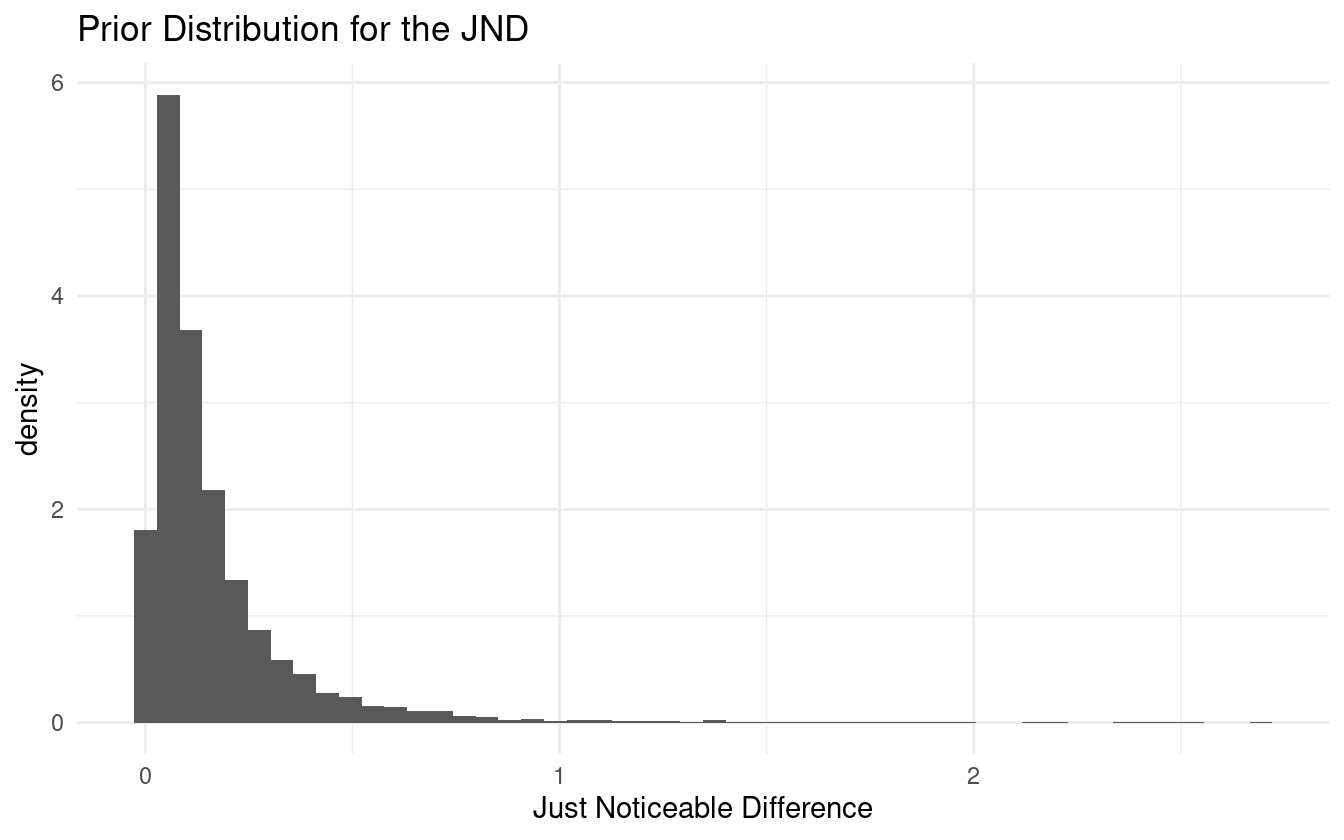
\includegraphics[width=0.85\linewidth]{040-application_files/figure-latex/ch041-Risky-Lion-1} \end{center}

With a prior for the JND, the prior for \(\beta\) can be determined:

\setstretch{1.0}

\[
jnd \sim \mathrm{Lognormal}(-2.3, 0.99^2) \Longleftrightarrow \frac{1}{jnd} \sim \mathrm{Lognormal}(2.3, 0.99^2)
\]

and

\[
\beta = \frac{\mathrm{logit}(0.84)}{jnd} \sim \mathrm{Lognormal}(2.8, 0.99^2)
\]

The priors do not need to be too exact. Rounding the parameters for \(\beta\), the simple model is:

\begin{align*}
  k_i &\sim \mathrm{Binomial}(n_i, p_i) \\
  \mathrm{logit}(p_i) &= \beta ( x_i - \alpha ) \\
  \alpha &\sim \mathcal{N}(0, 0.06^2) \\
  \beta &\sim \mathrm{Lognormal}(3, 1^2)
\end{align*}

and in \texttt{Stan}, the model code is:

\begin{Shaded}
\begin{Highlighting}[]
\KeywordTok{data}\NormalTok{ \{}
  \DataTypeTok{int}\NormalTok{ N;}
  \DataTypeTok{int}\NormalTok{ n[N];}
  \DataTypeTok{int}\NormalTok{ k[N];}
  \DataTypeTok{vector}\NormalTok{[N] x;}
\NormalTok{\}}
\KeywordTok{parameters}\NormalTok{ \{}
  \DataTypeTok{real}\NormalTok{ alpha;}
  \DataTypeTok{real}\NormalTok{\textless{}}\KeywordTok{lower}\NormalTok{=}\DecValTok{0}\NormalTok{\textgreater{} beta;}
\NormalTok{\}}
\KeywordTok{model}\NormalTok{ \{}
  \DataTypeTok{vector}\NormalTok{[N] p = beta * (x {-} alpha);}
\NormalTok{  alpha \textasciitilde{} normal(}\DecValTok{0}\NormalTok{, }\FloatTok{0.06}\NormalTok{);}
\NormalTok{  beta \textasciitilde{} lognormal(}\FloatTok{3.0}\NormalTok{, }\FloatTok{1.0}\NormalTok{);}
\NormalTok{  k \textasciitilde{} binomial\_logit(n, p);}
\NormalTok{\}}
\KeywordTok{generated quantities}\NormalTok{ \{}
  \DataTypeTok{vector}\NormalTok{[N] log\_lik;}
  \DataTypeTok{vector}\NormalTok{[N] k\_pred;}
  \DataTypeTok{vector}\NormalTok{[N] theta = beta * (x {-} alpha);}
  \DataTypeTok{vector}\NormalTok{[N] p = inv\_logit(theta);}
  \ControlFlowTok{for}\NormalTok{ (i }\ControlFlowTok{in} \DecValTok{1}\NormalTok{:N) \{}
\NormalTok{    log\_lik[i] = binomial\_logit\_lpmf(k[i] | n[i], theta[i]);}
\NormalTok{    k\_pred[i]  = binomial\_rng(n[i], p[i]);}
\NormalTok{  \}}
\NormalTok{\}}
\end{Highlighting}
\end{Shaded}

\setstretch{2.0}

Notice that the model block is nearly identical to the mathematical model specified above.

\emph{Construct Summary Functions}

The next step is to construct any relevant summary functions. Since the distribution of posterior PSS and JND values are needed for the summary statistics, it will be convenient to have a function that can take in the posterior samples for \(\alpha\) and \(\beta\) and return the PSS and JND values. We define \(Q\) as a more general function that takes in the two parameters and a target probability, \(\pi\), and returns the distribution of SOA values at \(\pi\).

\begin{equation}
  Q(\pi; \alpha, \beta) = \frac{\mathrm{logit(\pi)}}{\beta} + \alpha
  \label{eq:summfun1}
\end{equation}

The function can be defined in \texttt{R} as

\begin{Shaded}
\begin{Highlighting}[]
\NormalTok{Q }\OtherTok{\textless{}{-}} \ControlFlowTok{function}\NormalTok{(p, a, b) }\FunctionTok{qlogis}\NormalTok{(p) }\SpecialCharTok{/}\NormalTok{ b }\SpecialCharTok{+}\NormalTok{ a}
\end{Highlighting}
\end{Shaded}

With \(Q\), the PSS and JND can be calculated as

\setstretch{1.0}

\begin{align*}
  pss &= Q(0.5) \\
  jnd &= Q(0.84) - Q(0.5)
\end{align*}
\setstretch{2.0}

\emph{Simulate Bayesian Ensemble}

During this step, we simulate the Bayesian model and later feed the prior values into the summary functions in order to verify that there are no inconsistencies with domain knowledge. Since the model is fairly simple, we simulate directly in \texttt{R}.

\setstretch{1.0}

\begin{Shaded}
\begin{Highlighting}[]
\FunctionTok{set.seed}\NormalTok{(}\DecValTok{124}\NormalTok{)}
\NormalTok{n }\OtherTok{\textless{}{-}} \DecValTok{10000}

\NormalTok{a }\OtherTok{\textless{}{-}} \FunctionTok{rnorm}\NormalTok{(n, }\DecValTok{0}\NormalTok{, }\FloatTok{0.06}\NormalTok{)}
\NormalTok{b }\OtherTok{\textless{}{-}} \FunctionTok{rlnorm}\NormalTok{(n, }\FloatTok{3.0}\NormalTok{, }\DecValTok{1}\NormalTok{)}

\NormalTok{dat }\OtherTok{\textless{}{-}} \FunctionTok{with}\NormalTok{(av\_dat, }\FunctionTok{list}\NormalTok{(}\AttributeTok{N =}\NormalTok{ N, }\AttributeTok{x =}\NormalTok{ x, }\AttributeTok{n =}\NormalTok{ n)) }
\NormalTok{n\_obs }\OtherTok{\textless{}{-}} \FunctionTok{length}\NormalTok{(dat}\SpecialCharTok{$}\NormalTok{x)}

\NormalTok{idx }\OtherTok{\textless{}{-}} \FunctionTok{sample}\NormalTok{(}\DecValTok{1}\SpecialCharTok{:}\NormalTok{n, n\_obs, }\AttributeTok{replace =} \ConstantTok{TRUE}\NormalTok{)}
\NormalTok{probs }\OtherTok{\textless{}{-}} \FunctionTok{logistic}\NormalTok{(b[idx] }\SpecialCharTok{*}\NormalTok{ (dat}\SpecialCharTok{$}\NormalTok{x }\SpecialCharTok{{-}}\NormalTok{ a[idx]))}
\NormalTok{sim\_k }\OtherTok{\textless{}{-}} \FunctionTok{rbinom}\NormalTok{(n\_obs, dat}\SpecialCharTok{$}\NormalTok{n, probs)}
\end{Highlighting}
\end{Shaded}

\setstretch{2.0}

\emph{Prior Checks}

This step pertains to ensuring that prior estimates are consistent with domain expertise. We already did that in the model construction step by sampling values for the just noticeable difference. The first prior chosen was not producing JND estimates that were consistent with domain knowledge, so we adjusted accordingly.

Figure \ref{fig:ch041-prior-pf-plot} shows the distribution of prior psychometric functions derived from the simulated ensemble. There are a few very steep and very shallow curves, but the majority fall within a range that appears likely.

\begin{figure}

{\centering 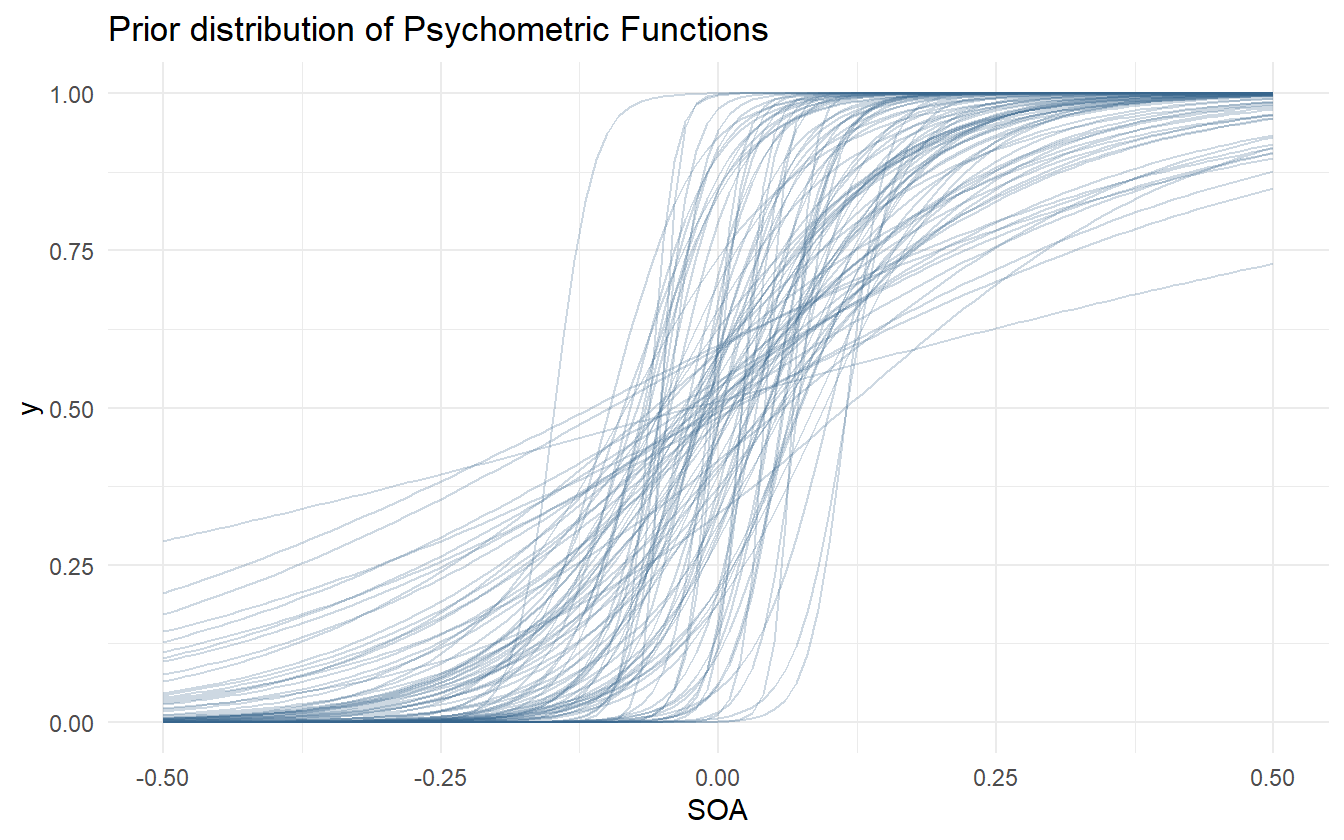
\includegraphics[width=0.85\linewidth]{040-application_files/figure-latex/ch041-prior-pf-plot-1} 

}

\caption{Prior distribution of psychometric functions using the priors for alpha and beta.}\label{fig:ch041-prior-pf-plot}
\end{figure}

Additionally most of the PSS values are within \(\pm 0.1\) with room to allow for some larger values. Let's check the prior distribution of PSS and JND values.

\begin{figure}

{\centering 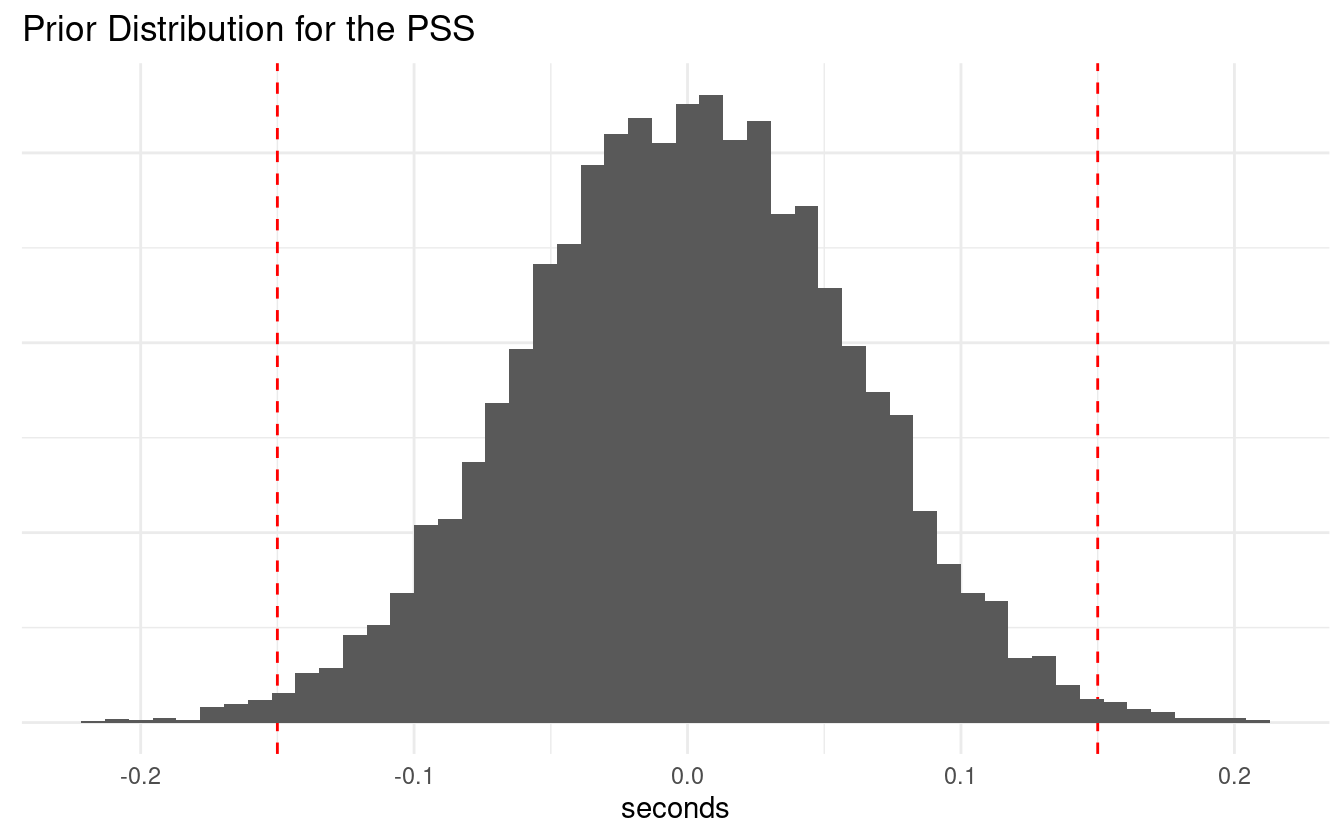
\includegraphics[width=0.85\linewidth]{040-application_files/figure-latex/ch041-prior-pss-plot-1} 

}

\caption{PSS prior distribution.}\label{fig:ch041-prior-pss-plot}
\end{figure}

\begin{figure}

{\centering 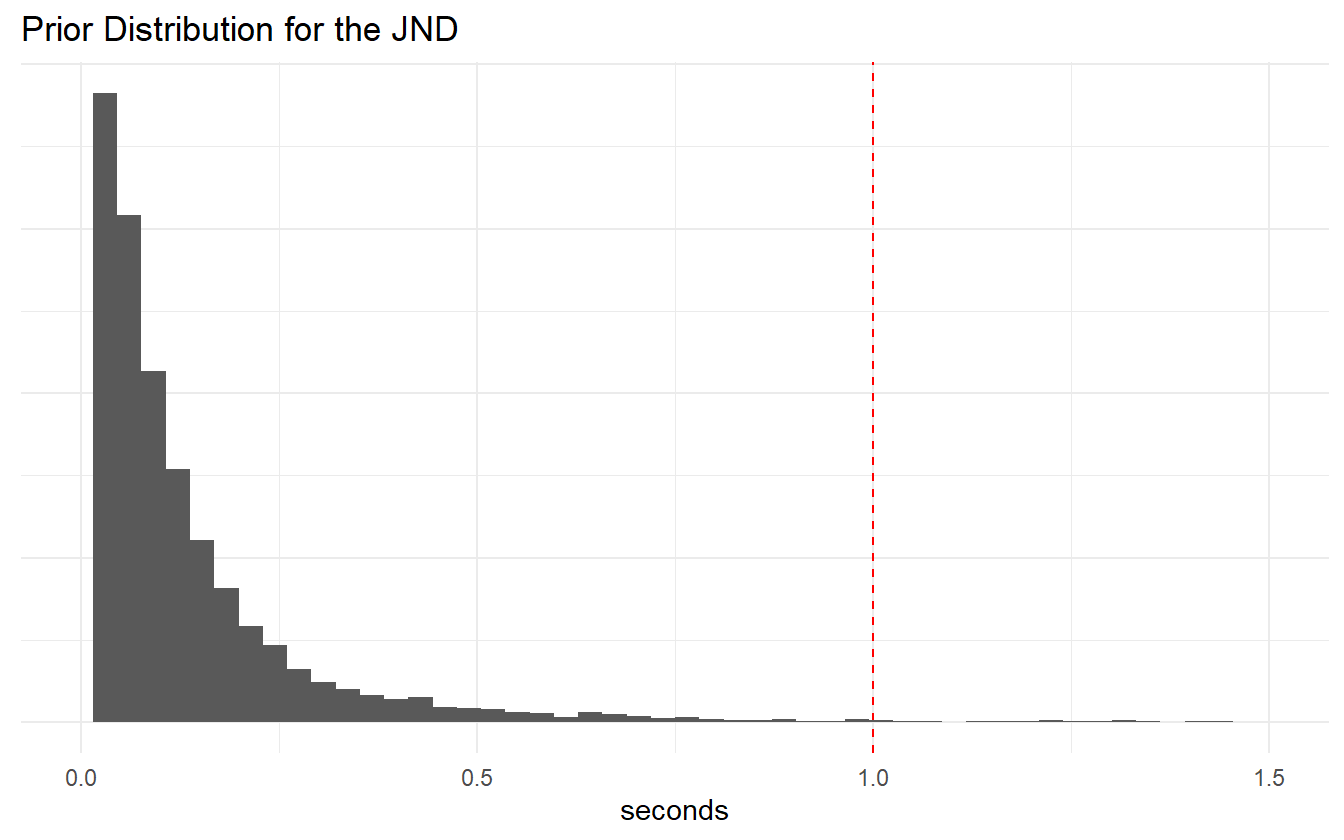
\includegraphics[width=0.85\linewidth]{040-application_files/figure-latex/ch041-prior-jnd-plot-1} 

}

\caption{JND prior distribution.}\label{fig:ch041-prior-jnd-plot}
\end{figure}

We are satisfied with the prior coverage of the PSS and JND values, and there are only a few samples that go beyond the extremes that were specified in the summary statistics step.

\emph{Configure Algorithm}

There are a few parameters that can be set for \texttt{Stan}. On the user side, the main parameters are the number of iterations, the number of warm-up iterations, the target acceptance rate, and the number of chains to run. By default, \texttt{Stan} will use half the number of iterations for warm-up and the other half for actual sampling. For now we use the default algorithm parameters in \texttt{Stan}, and will tweak them later if and when issues arise.

\emph{Fit Simulated Ensemble}

We now fit the model to the simulated data.

\setstretch{1.0}

\begin{Shaded}
\begin{Highlighting}[]
\NormalTok{sim\_dat }\OtherTok{\textless{}{-}} \FunctionTok{with}\NormalTok{(av\_dat, }\FunctionTok{list}\NormalTok{(}\AttributeTok{N =}\NormalTok{ N, }\AttributeTok{x =}\NormalTok{ x, }\AttributeTok{n =}\NormalTok{ n, }\AttributeTok{k =}\NormalTok{ sim\_k)) }
\NormalTok{m041 }\OtherTok{\textless{}{-}}\NormalTok{ rstan}\SpecialCharTok{::}\FunctionTok{sampling}\NormalTok{(m041\_stan, }\AttributeTok{data =}\NormalTok{ sim\_dat, }
                        \AttributeTok{chains =} \DecValTok{4}\NormalTok{, }\AttributeTok{cores =} \DecValTok{4}\NormalTok{, }\AttributeTok{refresh =} \DecValTok{0}\NormalTok{)}
\end{Highlighting}
\end{Shaded}

\setstretch{2.0}

\emph{Algorithmic Calibration}

To check the basic diagnostics of the model, we run the following code.

\setstretch{1.0}

\begin{Shaded}
\begin{Highlighting}[]
\FunctionTok{check\_hmc\_diagnostics}\NormalTok{(m041)}
\CommentTok{\#\textgreater{} }
\CommentTok{\#\textgreater{} Divergences:}
\CommentTok{\#\textgreater{} 0 of 4000 iterations ended with a divergence.}
\CommentTok{\#\textgreater{} }
\CommentTok{\#\textgreater{} Tree depth:}
\CommentTok{\#\textgreater{} 0 of 4000 iterations saturated the maximum tree depth of 10.}
\CommentTok{\#\textgreater{} }
\CommentTok{\#\textgreater{} Energy:}
\CommentTok{\#\textgreater{} E{-}BFMI indicated no pathological behavior.}
\end{Highlighting}
\end{Shaded}

\setstretch{2.0}

There is no undesirable behavior from this model, so next we check the summary statistics of the estimated parameters.

\begin{table}[!h]

\caption{\label{tab:ch041-Cloudy-Toupee}Summary statistics of the fitted Bayesian ensemble.}
\centering
\begin{tabular}[t]{lrrrrrrr}
\toprule
parameter & mean & se\_mean & sd & 2.5\% & 97.5\% & n\_eff & Rhat\\
\midrule
alpha & 0.0061 & 0.0001 & 0.0038 & -0.0012 & 0.0136 & 4039 & 0.9995\\
beta & 10.7681 & 0.0051 & 0.2404 & 10.3043 & 11.2313 & 2202 & 1.0003\\
\bottomrule
\end{tabular}
\end{table}

Both the \(\hat{R}\) and \(N_{\mathrm{eff}}\) look fine for both \(\alpha\) and \(\beta\), though it is slightly concerning that \(\alpha\) is centered relatively far from zero. This could just be due to sampling variance, so we will continue on to the next step.

\textbf{Post-Model, Post-Data}

\emph{Fit Observed Data}

All of the work up until now has been done without peaking at the observed data. We go ahead and run the data through the model.

\setstretch{1.0}

\begin{Shaded}
\begin{Highlighting}[]
\NormalTok{m041 }\OtherTok{\textless{}{-}} \FunctionTok{sampling}\NormalTok{(m041\_stan, }\AttributeTok{data =}\NormalTok{ obs\_dat, }
                 \AttributeTok{chains =} \DecValTok{4}\NormalTok{, }\AttributeTok{cores =} \DecValTok{4}\NormalTok{, }\AttributeTok{refresh =} \DecValTok{200}\NormalTok{)}
\end{Highlighting}
\end{Shaded}

\setstretch{2.0}

\emph{Diagnose Posterior Fit}

Here we repeat the diagnostic checks that were used after fitting the simulated data.

\setstretch{1.0}

\begin{Shaded}
\begin{Highlighting}[]
\FunctionTok{check\_hmc\_diagnostics}\NormalTok{(m041)}
\CommentTok{\#\textgreater{} }
\CommentTok{\#\textgreater{} Divergences:}
\CommentTok{\#\textgreater{} 0 of 4000 iterations ended with a divergence.}
\CommentTok{\#\textgreater{} }
\CommentTok{\#\textgreater{} Tree depth:}
\CommentTok{\#\textgreater{} 0 of 4000 iterations saturated the maximum tree depth of 10.}
\CommentTok{\#\textgreater{} }
\CommentTok{\#\textgreater{} Energy:}
\CommentTok{\#\textgreater{} E{-}BFMI indicated no pathological behavior.}
\end{Highlighting}
\end{Shaded}

\setstretch{2.0}

\begin{table}[!h]

\caption{\label{tab:ch041-Maroon-Oyster}Summary statistics of the fitted Bayesian ensemble.}
\centering
\begin{tabular}[t]{lrrrrrrr}
\toprule
parameter & mean & se\_mean & sd & 2.5\% & 97.5\% & n\_eff & Rhat\\
\midrule
alpha & 0.0373 & 0.0001 & 0.0043 & 0.029 & 0.0458 & 3765 & 1.000\\
beta & 8.4259 & 0.0039 & 0.1839 & 8.070 & 8.7897 & 2249 & 1.001\\
\bottomrule
\end{tabular}
\end{table}

There are no indications of an ill-behaved posterior fit. Let's also check the posterior distribution of \(\alpha\) and \(\beta\) against the prior density (\ref{fig:ch041-m041-posterior-alpha-beta}).

\begin{figure}

{\centering 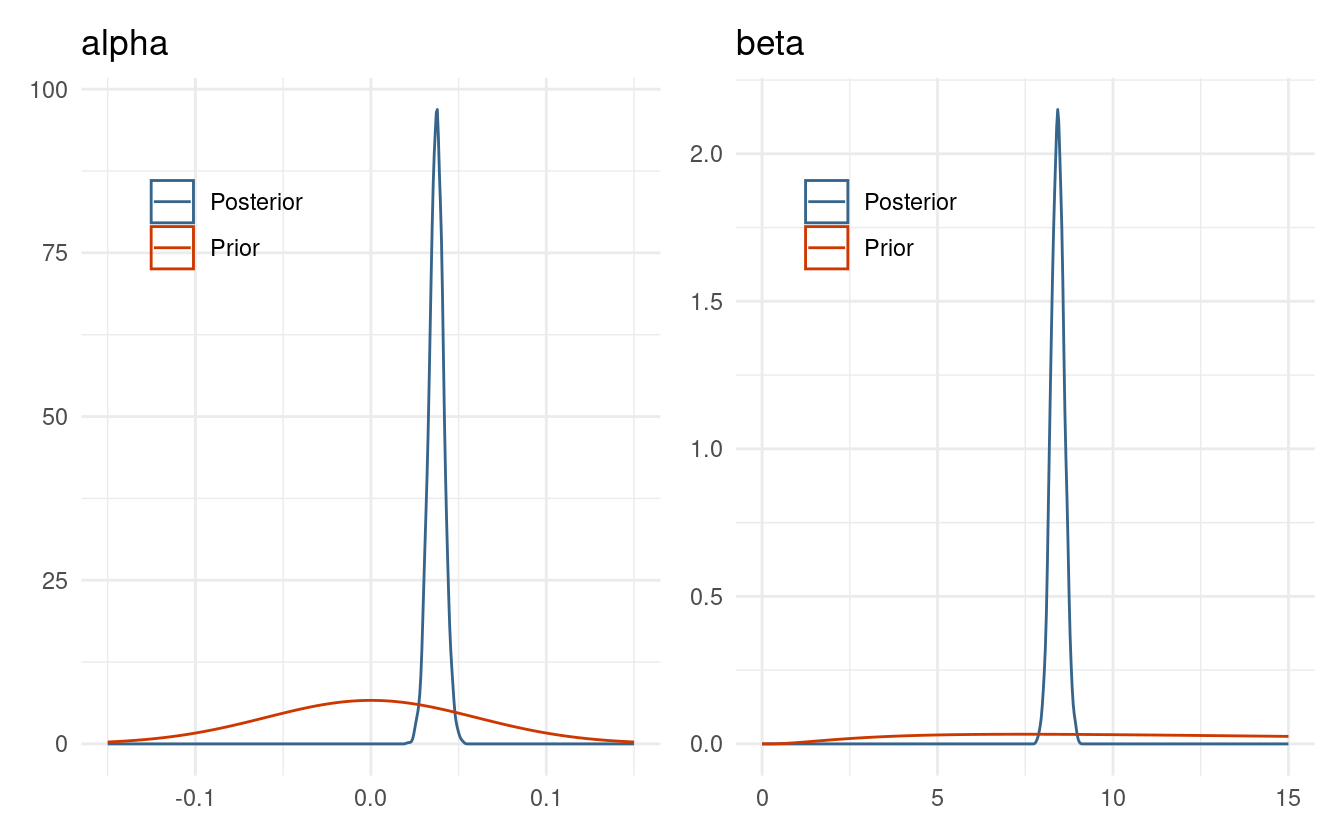
\includegraphics[width=0.85\linewidth]{040-application_files/figure-latex/ch041-m041-posterior-alpha-beta-1} 

}

\caption{Comparison of posterior distributions for alpha and beta to their respective prior distributions.}\label{fig:ch041-m041-posterior-alpha-beta}
\end{figure}

The posterior distributions for \(\alpha\) and \(\beta\) are well within the range determined by domain knowledge, and highly concentrated due to both the large amount of data and the fact that this is a completely pooled model -- all subject data is used to estimate the parameters. As expected, the prior for the JND could have been tighter with more weight below half a second compared to the one second limit used, but this is not prior information, so it is not prudent to change the prior in this manner after having seen the posterior. As a rule of thumb, priors should only be updated as motivated by domain expertise and not by the posterior distribution.

\emph{Posterior Retrodictive Checks}

It is time to run the posterior samples through the summary functions and then perform retrodictive checks. A retrodiction is using the posterior model to predict and compare to the observed data. This is simply done by drawing samples from the posterior and feeding in the observational data. This may be repeated to gain posterior predictive samples.

\setstretch{1.0}

\begin{Shaded}
\begin{Highlighting}[]
\NormalTok{posterior\_pss }\OtherTok{\textless{}{-}} \FunctionTok{Q}\NormalTok{(}\FloatTok{0.5}\NormalTok{, p041}\SpecialCharTok{$}\NormalTok{alpha, p041}\SpecialCharTok{$}\NormalTok{beta)}
\NormalTok{posterior\_jnd }\OtherTok{\textless{}{-}} \FunctionTok{Q}\NormalTok{(}\FloatTok{0.84}\NormalTok{, p041}\SpecialCharTok{$}\NormalTok{alpha, p041}\SpecialCharTok{$}\NormalTok{beta) }\SpecialCharTok{{-}}\NormalTok{ posterior\_pss}
\end{Highlighting}
\end{Shaded}

\setstretch{2.0}

\begin{figure}

{\centering 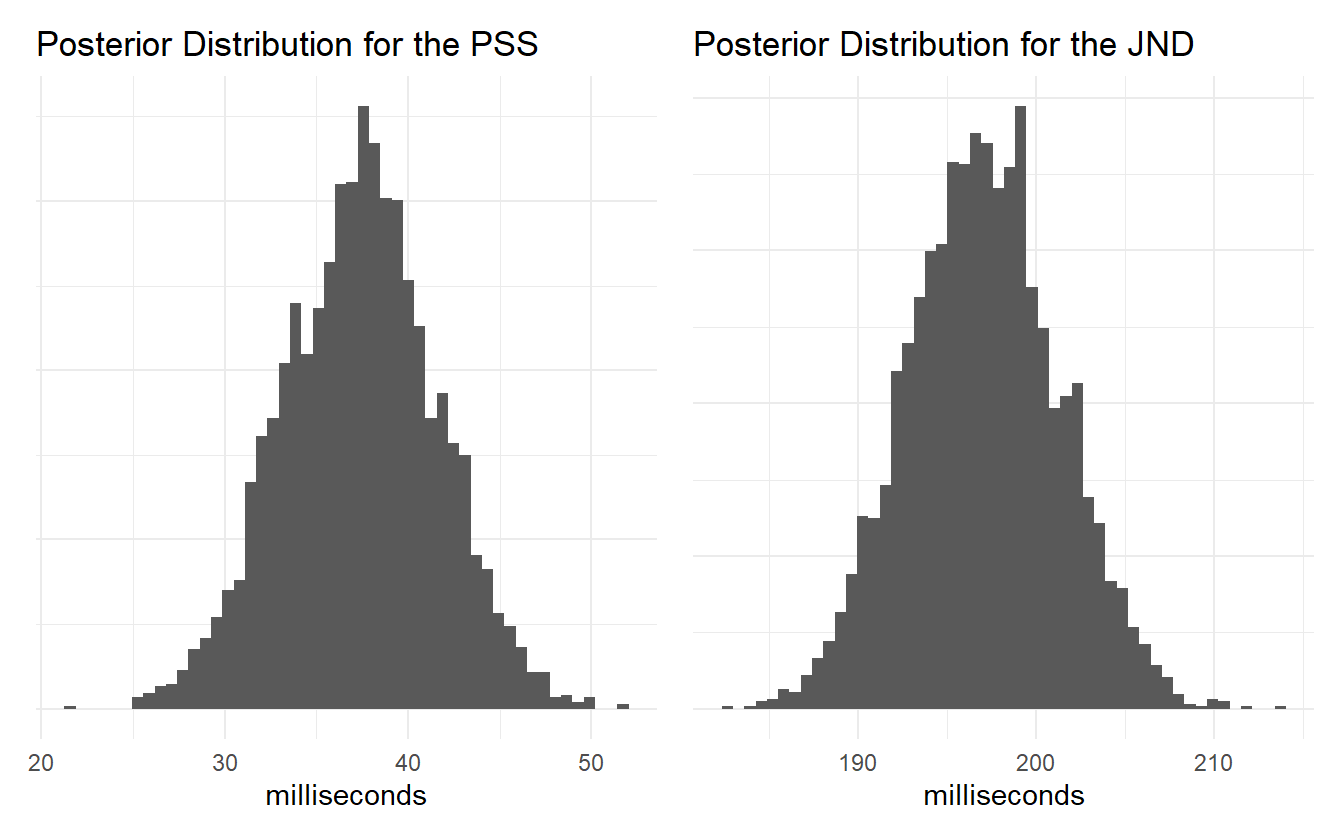
\includegraphics[width=0.85\linewidth]{040-application_files/figure-latex/ch041-posterior-pss-jnd-plot-1} 

}

\caption{Posterior distribution of the PSS and JND.}\label{fig:ch041-posterior-pss-jnd-plot}
\end{figure}

Neither of the posterior estimates for the PSS or JND exceed the extreme cutoffs set in the earlier steps, so we can be confident that the model is consistent with domain expertise. Note how simple it is to visualize and summarize the distribution of values for these measures. Using classical techniques like MLE might require using bootstrap methods to estimate the distribution of parameter values, or one might approximate the parameter distributions using the mean and standard error of the mean to simulate new values.

Next is to create the posterior predictive samples. We do this in two steps to better show how the distribution of posterior psychometric functions relates to the observed data, and then compare the observed data to the retrodictions. Figure \ref{fig:ch041-posterior-pf-plot} shows the result of the first step.

\begin{figure}

{\centering 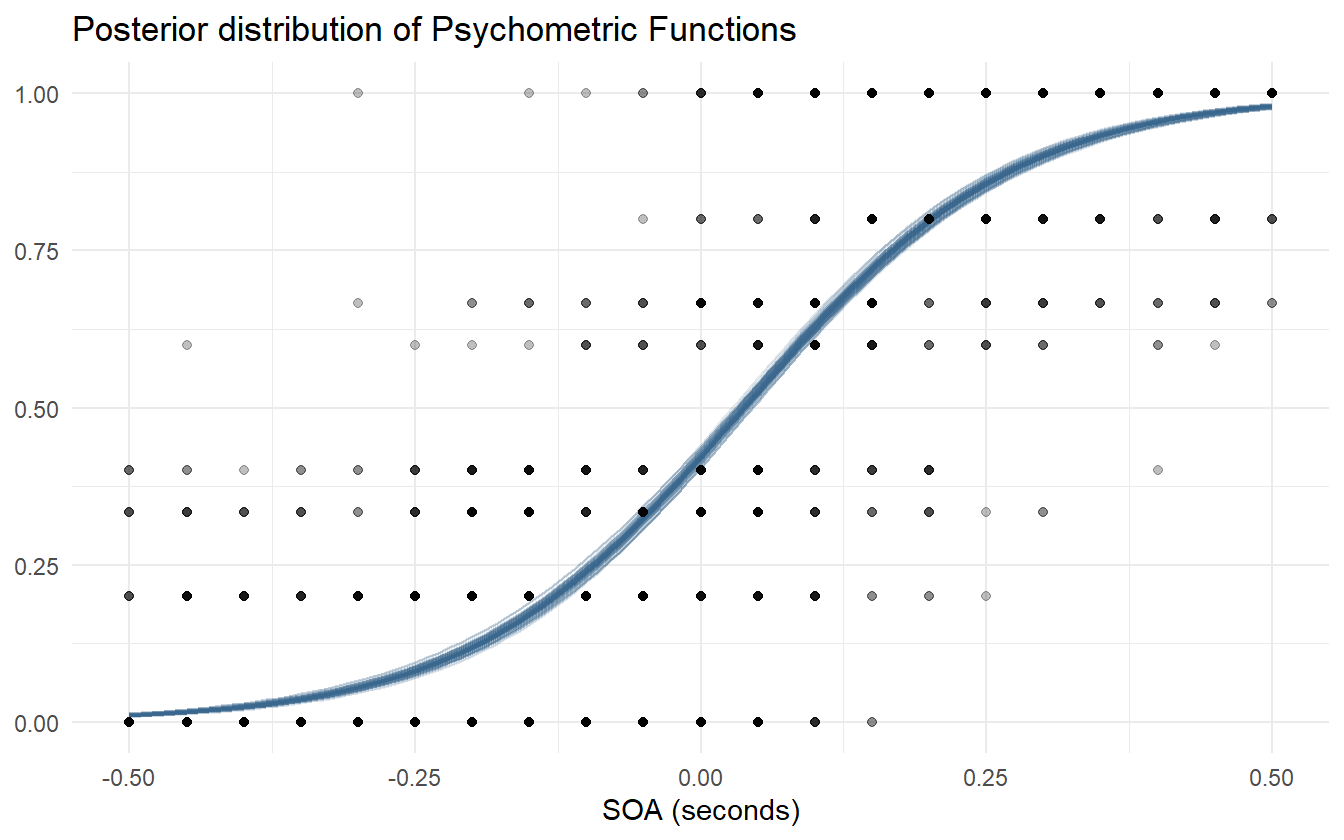
\includegraphics[width=0.85\linewidth]{040-application_files/figure-latex/ch041-posterior-pf-plot-1} 

}

\caption{Posterior distribution of psychometric functions using pooled observations.}\label{fig:ch041-posterior-pf-plot}
\end{figure}

Next we sample parameter values from the posterior distribution and use them to simulate a new data set. In the next iteration we show how to get \texttt{Stan} to automatically produce posterior predictive samples from the model fitting step. The results of the posterior predictions are shown in figure \ref{fig:ch041-obs-vs-retro-plot}.

\setstretch{1.0}

\begin{Shaded}
\begin{Highlighting}[]
\NormalTok{alpha }\OtherTok{\textless{}{-}} \FunctionTok{sample}\NormalTok{(p041}\SpecialCharTok{$}\NormalTok{alpha, n\_obs, }\AttributeTok{replace =} \ConstantTok{TRUE}\NormalTok{)}
\NormalTok{beta  }\OtherTok{\textless{}{-}} \FunctionTok{sample}\NormalTok{(p041}\SpecialCharTok{$}\NormalTok{beta, n\_obs, }\AttributeTok{replace =} \ConstantTok{TRUE}\NormalTok{)}
\NormalTok{logodds }\OtherTok{\textless{}{-}}\NormalTok{ beta }\SpecialCharTok{*}\NormalTok{ (av\_dat}\SpecialCharTok{$}\NormalTok{x }\SpecialCharTok{{-}}\NormalTok{ alpha)}
\NormalTok{probs }\OtherTok{\textless{}{-}} \FunctionTok{logistic}\NormalTok{(logodds)}
\NormalTok{sim\_k }\OtherTok{\textless{}{-}} \FunctionTok{rbinom}\NormalTok{(n\_obs, av\_dat}\SpecialCharTok{$}\NormalTok{n, probs)}
\end{Highlighting}
\end{Shaded}

\setstretch{2.0}

\begin{figure}

{\centering 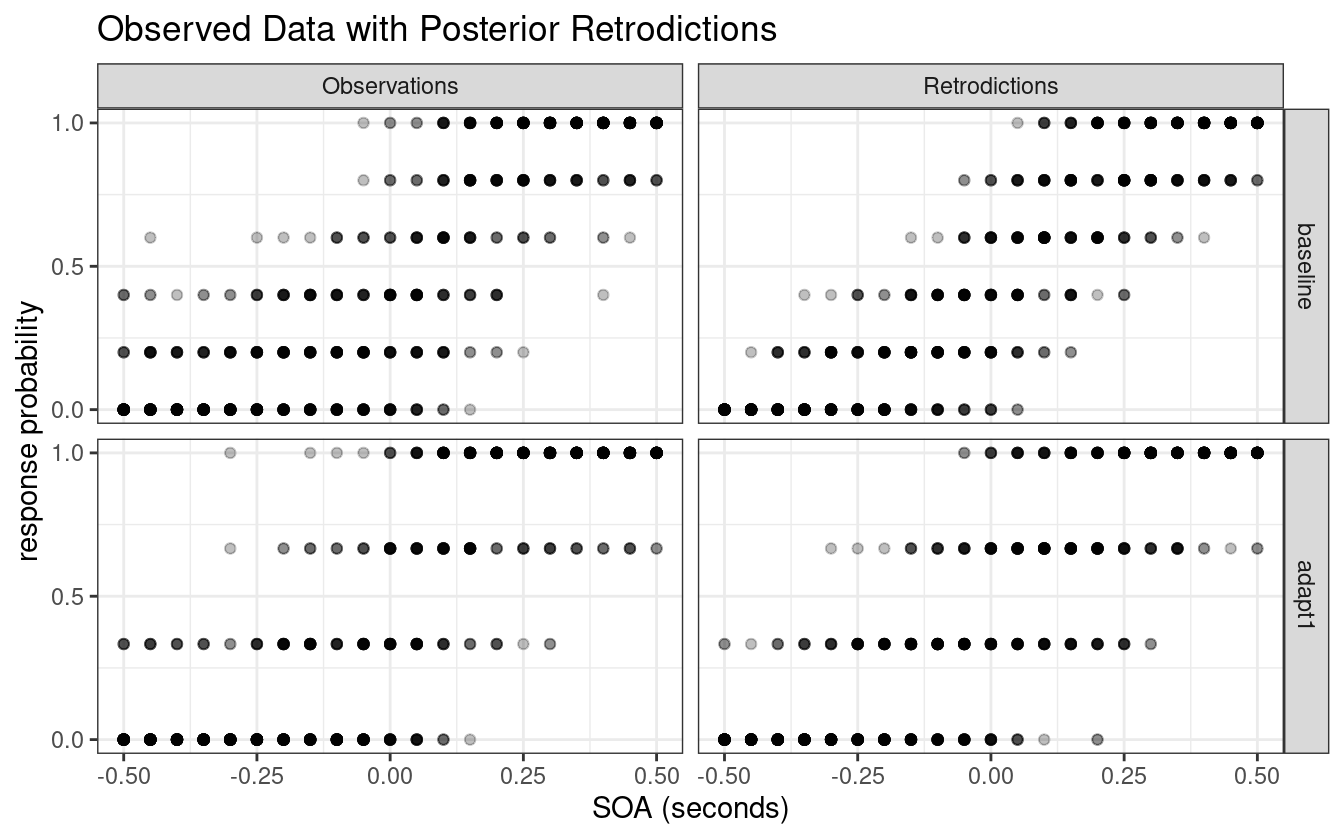
\includegraphics[width=0.85\linewidth]{040-application_files/figure-latex/ch041-obs-vs-retro-plot-1} 

}

\caption{Observed data compared to the posterior retrodictions. The data is post-stratified by block for easier visualization.}\label{fig:ch041-obs-vs-retro-plot}
\end{figure}

Let's be clear what the first iteration of this model describes. It is the average distribution of underlying psychometric functions across all subjects and blocks. It cannot tell us what the differences between pre- and post-adaptation blocks are, or what the variation between subjects is. It is useful in determining if the average value for the PSS is different from 0 or if the average JND is different from some other predetermined level. This model is still useful given the right question, but it cannot answer questions about group-level effects.

Figure \ref{fig:ch041-obs-vs-retro-plot} shows that the model captures the broad structure of the observed data, but is perhaps a bit under-dispersed in the tail ends of the SOA values. Besides this one issue, we are satisfied with the first iteration of this model and are ready to proceed to the next iteration.

\hypertarget{iter2}{%
\section{Iteration 2: adding age and block}\label{iter2}}

In this iteration we add the treatment and age groups into the model. There are no changes with the conceptual understanding of the experiment, and nothing to change with the observational space. As such we skip the first three steps and go to the model development step. As we build the model, the number of changes from one iteration to the next should go to zero as the model expands to become only as complex as necessary to answer the research questions.

\textbf{Post-Model, Pre-Data}

\emph{Develop Model}

To start, let's add in the treatment indicator and put off consideration of adding in the age group levels. In classical statistics, it is added as an indicator variable -- a zero or one -- for both the slope and intercept (varying slopes, varying intercepts model). Let \(trt\) be \(0\) if it is the pre-adaptation block and \(1\) if the observation comes from the post-adaptation block.

\setstretch{1.0}

\[\theta = \alpha + \alpha_{trt} \times trt + \beta \times x + \beta_{trt}\times trt \times x\]
\setstretch{2.0}

Now when an observation comes from the pre-adaptation block (\(trt=0\)) the linear predictor is given by

\setstretch{1.0}

\[\theta_{pre} = \alpha + \beta \times x\]
\setstretch{2.0}

and when an observation comes from the post-adaptation block (\(trt=1\)) the linear predictor is

\setstretch{1.0}

\[\theta_{post} = (\alpha + \alpha_{trt}) + (\beta + \beta_{trt}) \times x\]
\setstretch{2.0}

This may seem like a natural way to introduce an indicator variable, but it comes with serious implications. This model implies that there is more uncertainty about the post-adaptation block compared to the baseline block, and this is not necessarily true.

\setstretch{1.0}

\begin{align*}
\mathrm{Var}(\theta_{post}) &= \mathrm{Var}((\alpha + \alpha_{trt}) + (\beta + \beta_{trt}) \times x) \\
&= \mathrm{Var}(\alpha) + \mathrm{Var}(\alpha_{trt}) + x^2 \mathrm{Var}(\beta) + x^2\mathrm{Var}(\beta_{trt})
\end{align*}
\setstretch{2.0}

On the other hand, the variance of \(\theta_{pre}\) is:

\setstretch{1.0}

\[
\mathrm{Var}(\theta_{pre}) = \mathrm{Var}(\alpha) + x^2 \mathrm{Var}(\beta) \le \mathrm{Var}(\theta_{post})
\]
\setstretch{2.0}

Furthermore, the intercept, \(\alpha\), is no longer the average response probability at \(x=0\) for the entire data set, but is instead exclusively the average for the pre-adaptation block. This may not matter in certain analyses, but one nice property of multilevel models is the separation of population level estimates (fixed effects) and group level estimates (mixed effects).

Instead the treatment variable is introduced into the linear model as a factor variable. This means that each level in the treatment gets its own parameter, and this makes it easier to set priors when there are many levels in a group (such as for the subject level). The linear model, using equation \eqref{eq:linearform2}, with the treatment is written as:

\setstretch{1.0}

\begin{equation}
  \theta = (\beta + \beta_{trt[i]}) \left[x_i - (\alpha + \alpha_{trt[i]})\right]
  \label{eq:linearmodel2}
\end{equation}
\setstretch{2.0}

As more predictors and groups are added in, equation \eqref{eq:linearmodel2} becomes more difficult to read. What we do is break up the slope and intercept parameters and write the linear model as:

\setstretch{1.0}

\begin{align*}
\mu_\alpha &= \alpha + \alpha_{trt[i]} \\
\mu_\beta &= \beta + \beta_{trt[i]} \\
\theta &= \mu_\beta (x - \mu_\alpha)
\end{align*}
\setstretch{2.0}

In this way the combined parameters can be considered separately from the linear parameterization. Now we consider the priors for \(\alpha_{trt}\). Equation \eqref{eq:alpha-three-forms} shows three ways of adding in the block variable for \(\alpha\). The left equation is a standard single-level predictor, the center equation is the centered parameterization for a multilevel predictor, and the right equation is the non-centered parameterization for a multilevel predictor.

\setstretch{1.0}

\begin{equation}
  \begin{split}
    \mu_\alpha &= \alpha_{trt[i]} \\
    \alpha_{trt} &\sim \mathcal{N}(0, 0.06^2)
  \end{split}
\qquad
  \begin{split}
    \mu_\alpha &= \alpha_{trt[i]} \\
    \alpha &\sim \mathcal{N}(0, 0.06^2) \\
    \alpha_{trt} &\sim \mathcal{N}(\alpha, \sigma_{trt}^2) \\
    \sigma_{trt} &\sim \pi_{\sigma}
  \end{split}
\qquad
  \begin{split}
    \mu_\alpha &= \alpha + \alpha_{trt[i]} \\
    \alpha &\sim \mathcal{N}(0, 0.06^2) \\
    \alpha_{trt} &\sim \mathcal{N}(0, \sigma_{trt}^2) \\
    \sigma_{trt} &\sim \pi_{\sigma}
  \end{split}
\label{eq:alpha-three-forms}
\end{equation}
\setstretch{2.0}

In the center and right models of equation \eqref{eq:alpha-three-forms}, \(\alpha\) gets a fixed prior (the same as in the first iteration), and \(\alpha_{trt}\) gets a Gaussian prior with an adaptive variance term that is allowed to be learned from the data. This notation is compact, but \(\alpha_{trt}\) is two parameters - one each for the blocks. They both share the same variance term \(\sigma_{trt}\).

We will discuss selecting a prior for the variance term shortly. Instead of modeling \(\beta\) with a log-normal prior, we can sample from a normal distribution and take the exponential of it to produce a log-normal distribution:

\setstretch{1.0}

\begin{align*}
X &\sim \mathcal{N}(3, 1^2) \\
Y &= \exp\left(X\right) \Longleftrightarrow Y \sim \mathrm{Lognormal(3, 1^2)}
\end{align*}
\setstretch{2.0}

This is the non-centered parameterization of the log-normal distribution, and the motivation behind this parameterization is that it is now easier to include new slope variables as an additive affect. If both \(\beta\) and \(\beta_{trt}\) are specified with Gaussian priors, then the exponential of the sum will be a log-normal distribution. The model now becomes:

\setstretch{1.0}

\begin{equation}
\begin{split}
k_i &\sim \mathrm{Binomial}(n_i, p_i) \\
\mathrm{logit}(p_i) &= \exp(\mu_\beta) (x_i - \mu_\alpha) \\
\mu_\alpha &= \alpha + \alpha_{trt[i]} \\
\mu_\beta &= \beta + \beta_{trt[i]} \\
\alpha &\sim \mathcal{N}(0, 0.06^2) \\
\alpha_{trt} &\sim \mathcal{N}(0, \sigma_{trt}^2) \\
\beta &\sim \mathcal{N}(3, 1^2) \\
\beta_{trt} &\sim \mathcal{N}(0, \gamma_{trt}^2) \\
\sigma_{trt} &\sim \pi_{\sigma} \\
\gamma_{trt} &\sim \pi_{\gamma}
\end{split}
\label{eq:iter2-partial-model}
\end{equation}
\setstretch{2.0}

Deciding on priors for the variance term requires some careful consideration. In one sense, the variance term is the within-group variance. \citet{gelman2006prior} recommends that for multilevel models with groups with less than say 5 levels to use a half-Cauchy prior. This weakly informative prior still has a regularizing affect and dissuades larger variance estimates. Even though the treatment group only has two levels, there is still value in specifying an adaptive prior for them, and there is enough data for each treatment so that partial pooling won't have as extreme of a regularizing effect.

\setstretch{1.0}

\begin{align*}
\sigma_{trt} &\sim \mathrm{HalfCauchy}(0, 1) \\
\gamma_{trt} &\sim \mathrm{HalfCauchy}(0, 1)
\end{align*}
\setstretch{2.0}

We add in the age group level effects to \eqref{eq:iter2-partial-model} and specify their variance terms:

\setstretch{1.0}

\begin{equation}
\begin{split}
k_i &\sim \mathrm{Binomial}(n_i, p_i) \\
\mathrm{logit}(p_i) &= \exp(\mu_\beta) (x_i - \mu_\alpha) \\
\mu_\alpha &= \alpha + \alpha_{trt[i]} + \alpha_{G[i]} \\
\mu_\beta &= \beta + \beta_{trt[i]} + \beta_{G[i]} \\
\alpha &\sim \mathcal{N}(0, 0.06^2) \\
\alpha_{trt} &\sim \mathcal{N}(0, \sigma_{trt}^2) \\
\alpha_{G} &\sim \mathcal{N}(0, \tau_{trt}^2) \\
\beta &\sim \mathcal{N}(3, 1^2) \\
\beta_{trt} &\sim \mathcal{N}(0, \gamma_{trt}^2) \\
\beta_{G} &\sim \mathcal{N}(0, \nu_{G}^2) \\
\sigma_{trt}, \gamma_{trt} &\sim \mathrm{HalfCauchy}(0, 1) \\
\tau_{G}, \nu_{G}  &\sim \mathrm{HalfCauchy}(0, 2)
\end{split}
\label{eq:iter2-model}
\end{equation}
\setstretch{2.0}

The \texttt{Stan} code corresponding to model \eqref{eq:iter2-model} is becoming quite long, so we omit it from here on out. The final \texttt{Stan} model code may be found in the \protect\hyperlink{code}{supplementary code} section of the appendix.

\textbf{Post-Model, Post-Data}

\emph{Fit Observed Data}

We skip the prior checks and use the observed data to configure the algorithm and diagnose the posterior fit.

\setstretch{1.0}

\begin{Shaded}
\begin{Highlighting}[]
\NormalTok{m042 }\OtherTok{\textless{}{-}} \FunctionTok{sampling}\NormalTok{(m042\_stan, }\AttributeTok{data =}\NormalTok{ obs\_dat, }\AttributeTok{seed =} \DecValTok{124}\NormalTok{,}
                 \AttributeTok{chains =} \DecValTok{4}\NormalTok{, }\AttributeTok{cores =} \DecValTok{4}\NormalTok{, }\AttributeTok{refresh =} \DecValTok{100}\NormalTok{)}
\end{Highlighting}
\end{Shaded}

\setstretch{2.0}

\emph{Diagnose Posterior Fit}

\setstretch{1.0}

\begin{Shaded}
\begin{Highlighting}[]
\FunctionTok{check\_hmc\_diagnostics}\NormalTok{(m042)}
\CommentTok{\#\textgreater{} }
\CommentTok{\#\textgreater{} Divergences:}
\CommentTok{\#\textgreater{} 4 of 4000 iterations ended with a divergence (0.1\%).}
\CommentTok{\#\textgreater{} Try increasing \textquotesingle{}adapt\_delta\textquotesingle{} to remove the divergences.}
\CommentTok{\#\textgreater{} }
\CommentTok{\#\textgreater{} Tree depth:}
\CommentTok{\#\textgreater{} 0 of 4000 iterations saturated the maximum tree depth of 10.}
\CommentTok{\#\textgreater{} }
\CommentTok{\#\textgreater{} Energy:}
\CommentTok{\#\textgreater{} E{-}BFMI indicated no pathological behavior.}
\end{Highlighting}
\end{Shaded}

\setstretch{2.0}

As well as the 4 divergent transitions, there is also a message about the effective sample size (ESS) being too low. The recommended prescription for low ESS is to run the chains for more iterations. The posterior summary shows that \(N_{\mathrm{eff}}\) is low for the age group level parameters (table \ref{tab:ch042-Liquid-Strawberry-Eagle}).

\begin{table}[!h]

\caption{\label{tab:ch042-Liquid-Strawberry-Eagle}Summary statistics of the second iteration.}
\centering
\begin{tabular}[t]{lrrrrrrr}
\toprule
parameter & mean & se\_mean & sd & 2.5\% & 97.5\% & n\_eff & Rhat\\
\midrule
a & 0.0222 & 0.0014 & 0.0412 & -0.0683 & 0.1024 & 824.6 & 1.002\\
aG[1] & -0.0009 & 0.0012 & 0.0313 & -0.0531 & 0.0714 & 703.5 & 1.003\\
aG[2] & 0.0274 & 0.0012 & 0.0316 & -0.0218 & 0.0990 & 698.3 & 1.003\\
aG[3] & -0.0078 & 0.0012 & 0.0311 & -0.0609 & 0.0609 & 714.3 & 1.004\\
b & 2.4114 & 0.0216 & 0.5665 & 1.4902 & 3.8499 & 688.2 & 1.003\\
\addlinespace
bG[1] & 0.0030 & 0.0170 & 0.2942 & -0.7681 & 0.5013 & 301.3 & 1.004\\
bG[2] & 0.0538 & 0.0170 & 0.2940 & -0.7101 & 0.5499 & 299.9 & 1.004\\
bG[3] & -0.2223 & 0.0172 & 0.2955 & -1.0150 & 0.2597 & 296.9 & 1.004\\
\bottomrule
\end{tabular}
\end{table}

We can return to the algorithm configuration step and increase the number of iterations and warm-up iterations, as well as increase the adapt delta parameter to reduce the number of divergent transitions (which really isn't a problem right now).

Another technique we can employ is non-centered parameterization. Model \eqref{eq:iter2-model} uses non-centered parameterization for \(\mu_\alpha\) and \(\mu_\beta\). Other parameters, especially the variance terms, can also benefit from non-centered parameterization. Model \eqref{eq:iter2-model-nc} shows the results of reparameterizing:

\setstretch{1.0}

\begin{equation}
\begin{split}
k_i &\sim \mathrm{Binomial}(n_i, p_i) \\
\mathrm{logit}(p_i) &= \exp(\mu_\beta) (x_i - \mu_\alpha) \\
\mu_\alpha &= \alpha + \alpha_{trt[i]} + \alpha_{G[i]} \\
\mu_\beta &= \beta + \beta_{trt[i]} + \beta_{G[i]} \\
\hat{\alpha}, \hat{\alpha}_{trt}, \hat{\alpha}_{G} &\sim \mathcal{N}(0, 1^2) \\
\hat{\beta}, \hat{\beta}_{trt}, \hat{\beta}_{G} &\sim \mathcal{N}(0, 1^2) \\
\hat{\sigma}_{trt}, \hat{\gamma}_{trt}, \hat{\tau}_{G}, \hat{\nu}_{G} &\sim \mathcal{U}(0, \pi/2) \\
\alpha &= 0.06 \cdot \hat{\alpha} \\
\alpha_{trt} &= \sigma_{trt} \cdot \hat{\alpha}_{trt} \\
\alpha_{G} &= \gamma_{G} \cdot \hat{\alpha}_{G} \\
\sigma_{trt} &= \tan(\hat{\sigma}_{trt}) \\
\gamma_{G} &= \tan(\hat{\gamma}_{G}) \\
\beta &= 3 + 1 \cdot \hat{\beta} \\
\beta_{trt} &= \tau_{trt} \cdot \hat{\beta}_{trt} \\
\beta_{G} &= \nu_{G} \cdot \hat{\beta}_{G} \\
\tau_{trt} &= \tan(\hat{\tau}_{trt}) \\
\nu_{G} &= \tan(\hat{\nu}_{G})
\end{split}
\label{eq:iter2-model-nc}
\end{equation}
\setstretch{2.0}

\emph{Develop Model}

The model changes consist of using the non-centered parameterizations discussed in the previous step.

As an aside, a multilevel model can be fit in \texttt{R} using \texttt{lme4::glmer}, \texttt{brms::brm}, or \texttt{rstanarm::stan\_glmer}, and they all use the same notation to specify the model. The notation is very compact, but easy to unpack. Values not in a grouping term are fixed effects and values in a grouping term (e.g.~\texttt{(1\ +\ x\ \textbar{}\ G)}) are mixed or random effects depending on which textbook you read.

\setstretch{1.0}

\begin{Shaded}
\begin{Highlighting}[]
\NormalTok{f }\OtherTok{\textless{}{-}} \FunctionTok{formula}\NormalTok{(k}\SpecialCharTok{|}\NormalTok{n }\SpecialCharTok{\textasciitilde{}} \DecValTok{1} \SpecialCharTok{+}\NormalTok{ x }\SpecialCharTok{+}\NormalTok{ (}\DecValTok{1} \SpecialCharTok{+}\NormalTok{ x }\SpecialCharTok{|}\NormalTok{ G) }\SpecialCharTok{+}\NormalTok{ (}\DecValTok{1} \SpecialCharTok{+}\NormalTok{ x }\SpecialCharTok{|}\NormalTok{ trt))}

\NormalTok{lme4}\SpecialCharTok{::}\FunctionTok{glmer}\NormalTok{(f, }\AttributeTok{data =}\NormalTok{ data, }\AttributeTok{family =} \FunctionTok{binomial}\NormalTok{(}\StringTok{"logit"}\NormalTok{))}
\NormalTok{rstanarm}\SpecialCharTok{::}\FunctionTok{stan\_glmer}\NormalTok{(f, }\AttributeTok{data =}\NormalTok{ data, }\AttributeTok{family =} \FunctionTok{binomial}\NormalTok{(}\StringTok{"logit"}\NormalTok{))}
\NormalTok{brms}\SpecialCharTok{::}\FunctionTok{brm}\NormalTok{(f, }\AttributeTok{data =}\NormalTok{ data, }\AttributeTok{family =} \FunctionTok{binomial}\NormalTok{(}\StringTok{"logit"}\NormalTok{))}
\end{Highlighting}
\end{Shaded}

\setstretch{2.0}

The simpler notation and compactness of these methods are very attractive, and for certain analyses they may be more than sufficient. The goal here is to decide early on if these methods satisfy the model adequacy, and to use more flexible modeling tools like \texttt{Stan} if necessary.

\emph{Fit Observed Data}

This time we fit the model with the non-centered parameterization. Since this model is sampling from intermediate parameters, we can choose to keep only the transformed parameters.

\setstretch{1.0}

\begin{Shaded}
\begin{Highlighting}[]
\NormalTok{m042nc }\OtherTok{\textless{}{-}} \FunctionTok{sampling}\NormalTok{(m042nc\_stan, }\AttributeTok{data =}\NormalTok{ obs\_dat, }\AttributeTok{seed =} \DecValTok{143}\NormalTok{,}
                   \AttributeTok{iter =} \DecValTok{4000}\NormalTok{, }\AttributeTok{warmup =} \DecValTok{2000}\NormalTok{, }\AttributeTok{pars =}\NormalTok{ keep\_pars,}
                   \AttributeTok{control =} \FunctionTok{list}\NormalTok{(}\AttributeTok{adapt\_delta =} \FloatTok{0.95}\NormalTok{), }\AttributeTok{thin =} \DecValTok{2}\NormalTok{,}
                   \AttributeTok{chains =} \DecValTok{4}\NormalTok{, }\AttributeTok{cores =} \DecValTok{4}\NormalTok{, }\AttributeTok{refresh =} \DecValTok{100}\NormalTok{)}
\end{Highlighting}
\end{Shaded}

\setstretch{2.0}

\emph{Diagnose Posterior Fit}

\setstretch{1.0}

\begin{Shaded}
\begin{Highlighting}[]
\FunctionTok{check\_hmc\_diagnostics}\NormalTok{(m042nc)}
\CommentTok{\#\textgreater{} }
\CommentTok{\#\textgreater{} Divergences:}
\CommentTok{\#\textgreater{} 32 of 4000 iterations ended with a divergence (0.8\%).}
\CommentTok{\#\textgreater{} Try increasing \textquotesingle{}adapt\_delta\textquotesingle{} to remove the divergences.}
\CommentTok{\#\textgreater{} }
\CommentTok{\#\textgreater{} Tree depth:}
\CommentTok{\#\textgreater{} 0 of 4000 iterations saturated the maximum tree depth of 10.}
\CommentTok{\#\textgreater{} }
\CommentTok{\#\textgreater{} Energy:}
\CommentTok{\#\textgreater{} E{-}BFMI indicated no pathological behavior.}
\end{Highlighting}
\end{Shaded}

\setstretch{2.0}

There are still a few divergent transitions (\(<1\%\)), but the effective sample size increased significantly (table \ref{tab:ch042-Bleeding-Tuna}).

\begin{table}[!h]

\caption{\label{tab:ch042-Bleeding-Tuna}Summary statistics of the second iteration with non-centered parameterization.}
\centering
\begin{tabular}[t]{lrrrrrrr}
\toprule
parameter & mean & se\_mean & sd & 2.5\% & 97.5\% & n\_eff & Rhat\\
\midrule
a & 0.0192 & 0.0008 & 0.0419 & -0.0744 & 0.0956 & 2509 & 1.0005\\
aG[1] & -0.0025 & 0.0006 & 0.0326 & -0.0636 & 0.0739 & 2737 & 1.0014\\
aG[2] & 0.0262 & 0.0006 & 0.0328 & -0.0342 & 0.1044 & 2644 & 1.0014\\
aG[3] & -0.0093 & 0.0006 & 0.0326 & -0.0713 & 0.0652 & 2752 & 1.0011\\
aT[1] & 0.0185 & 0.0009 & 0.0425 & -0.0546 & 0.1242 & 2338 & 1.0005\\
\addlinespace
aT[2] & 0.0039 & 0.0009 & 0.0419 & -0.0679 & 0.1089 & 2404 & 1.0005\\
b & 2.3841 & 0.0115 & 0.5284 & 1.4762 & 3.6952 & 2109 & 1.0010\\
bG[1] & 0.0170 & 0.0049 & 0.2730 & -0.6323 & 0.4979 & 3106 & 1.0004\\
bG[2] & 0.0678 & 0.0049 & 0.2728 & -0.5773 & 0.5671 & 3113 & 1.0005\\
bG[3] & -0.2075 & 0.0050 & 0.2741 & -0.8506 & 0.2767 & 3026 & 1.0004\\
\addlinespace
bT[1] & -0.2764 & 0.0106 & 0.4914 & -1.6338 & 0.5427 & 2141 & 0.9999\\
bT[2] & -0.0501 & 0.0106 & 0.4909 & -1.4120 & 0.7778 & 2125 & 1.0000\\
\bottomrule
\end{tabular}
\end{table}

A more direct way to compare the efficiency is through the ratio of \(N_{\mathrm{eff}} / N\) (figure \ref{fig:ch042-Remote-Longitude}).

\begin{figure}

{\centering 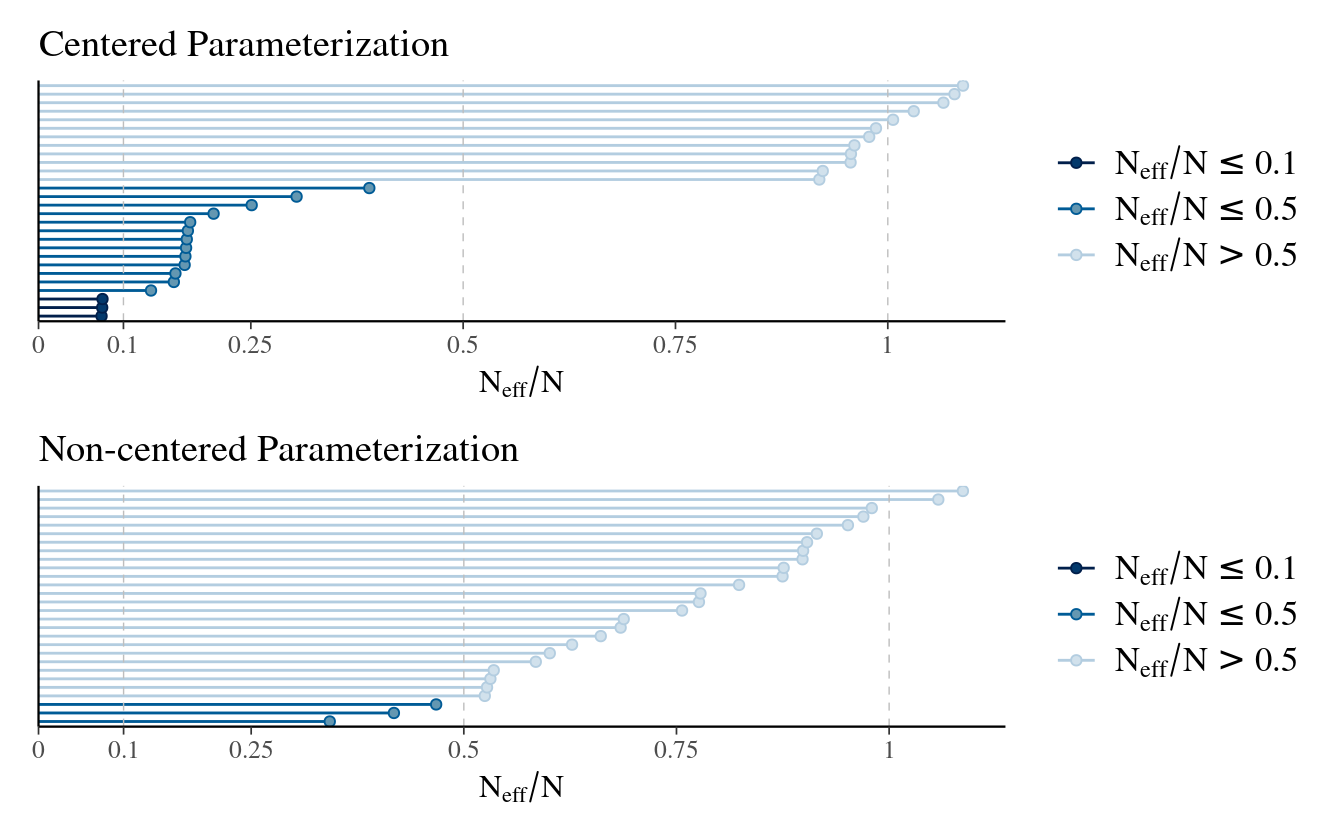
\includegraphics[width=0.85\linewidth]{040-application_files/figure-latex/ch042-Remote-Longitude-1} 

}

\caption{Model efficiency as measured by the N\_eff/N ratio.}\label{fig:ch042-Remote-Longitude}
\end{figure}

Figure \ref{fig:ch042-traceplot-m042nc} shows the trace plot for the slope and intercept parameters. Each chain looks like it is sampling around the same average value as the others with identical spreads (stationary and homoscedastic). This also helps to solidify the idea that the \(\hat{R}\) statistic is the measure of between chain variance compared to cross chain variance.

\begin{figure}

{\centering 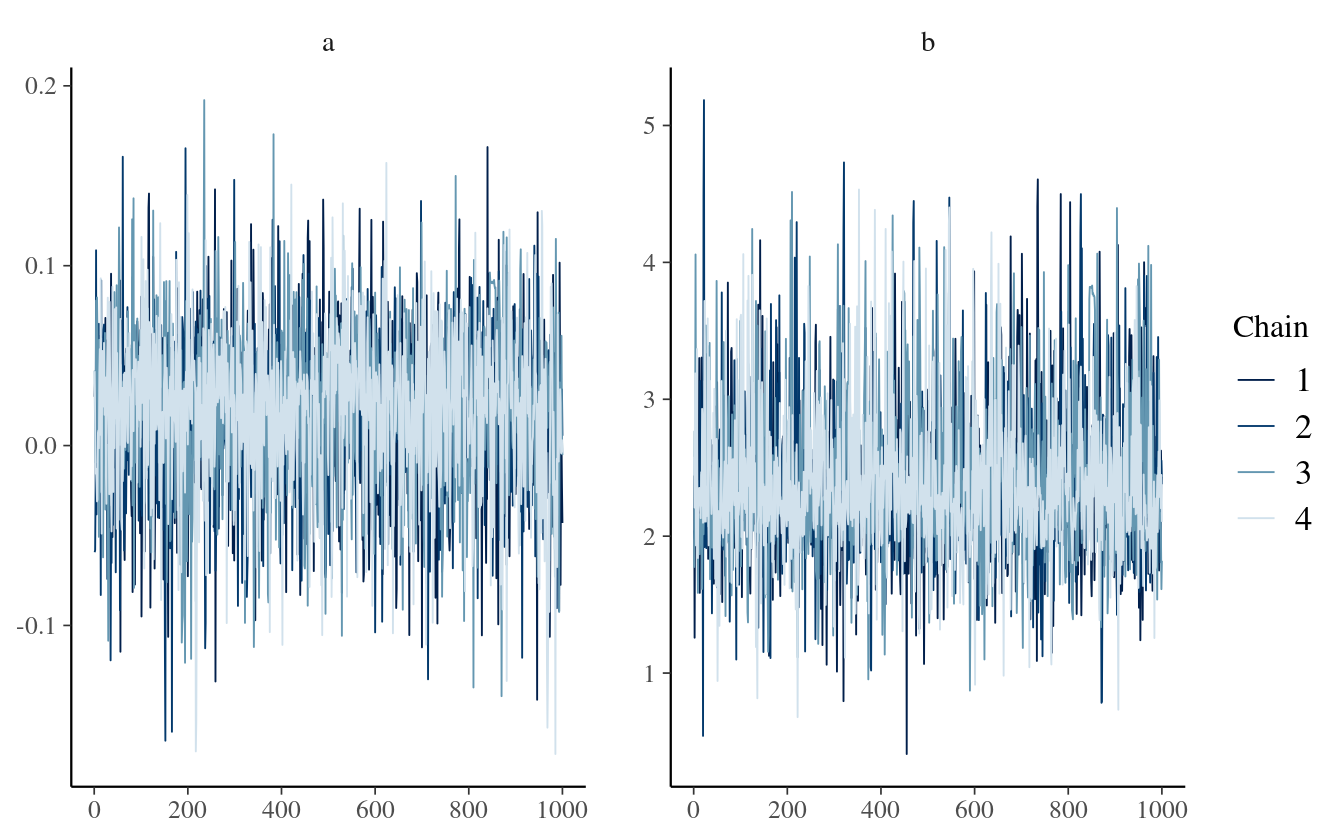
\includegraphics[width=0.85\linewidth]{040-application_files/figure-latex/ch042-traceplot-m042nc-1} 

}

\caption{Traceplot for the slope and intercept parameters.}\label{fig:ch042-traceplot-m042nc}
\end{figure}

The chains displayed in figure \ref{fig:ch042-traceplot-m042nc} are healthy, as well as for the other parameters not shown. Since there are no algorithmic issues, we proceed to the posterior retrodictive checks.

\emph{Posterior Retrodictive Checks}

We now have estimates for the age groups and the treatment. The posterior estimates for the PSS and JND are shown in figure \ref{fig:ch042-posterior-pss-jnd-plot}. There are many ways to visualize and compare the distributions across age groups and conditions that depend on what question is being asked. If for example the question is ``what is the qualitative difference between pre- and post-adaptation across age groups?'', then figure \ref{fig:ch042-posterior-pss-jnd-plot} could answer that because it juxtaposes the two blocks in the same panel. We will consider alternative ways of arranging the plots in \protect\hyperlink{results}{chapter 5}.

\begin{figure}

{\centering 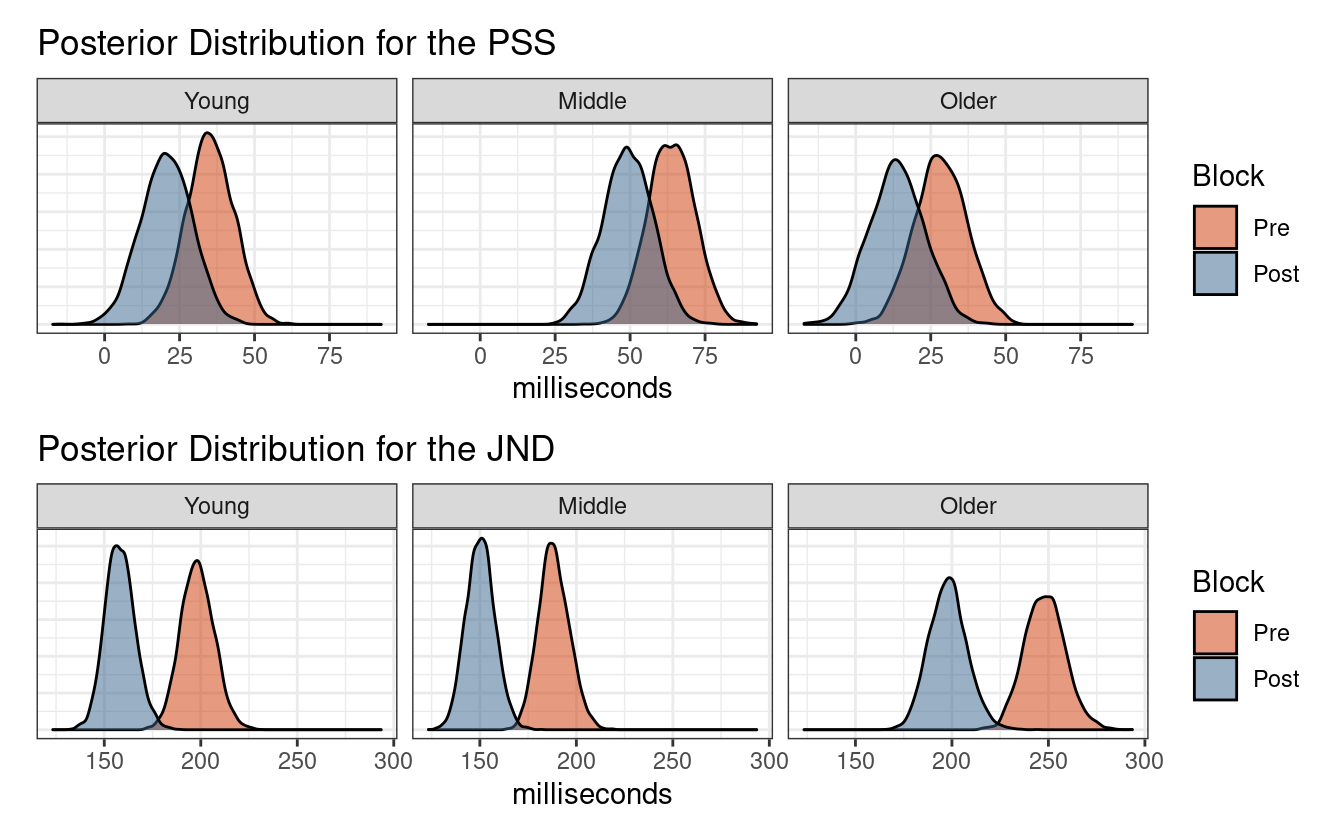
\includegraphics[width=0.85\linewidth]{040-application_files/figure-latex/ch042-posterior-pss-jnd-plot-1} 

}

\caption{Posterior distribution of the PSS and JND.}\label{fig:ch042-posterior-pss-jnd-plot}
\end{figure}

For the posterior retrodictions, we can do something similar to last time. We had \texttt{Stan} perform posterior predictive sampling during the fitting step. This was achieved by adding a \texttt{generated\ quantities} block to the code that takes the posterior samples for the parameters, and then randomly generates a value from a binomial distribution for each observation in the data. In effect, we now have \(4000\) simulated data sets. We only need one data set to compare to the observed data, so it is selected randomly from the posterior.

\begin{figure}

{\centering 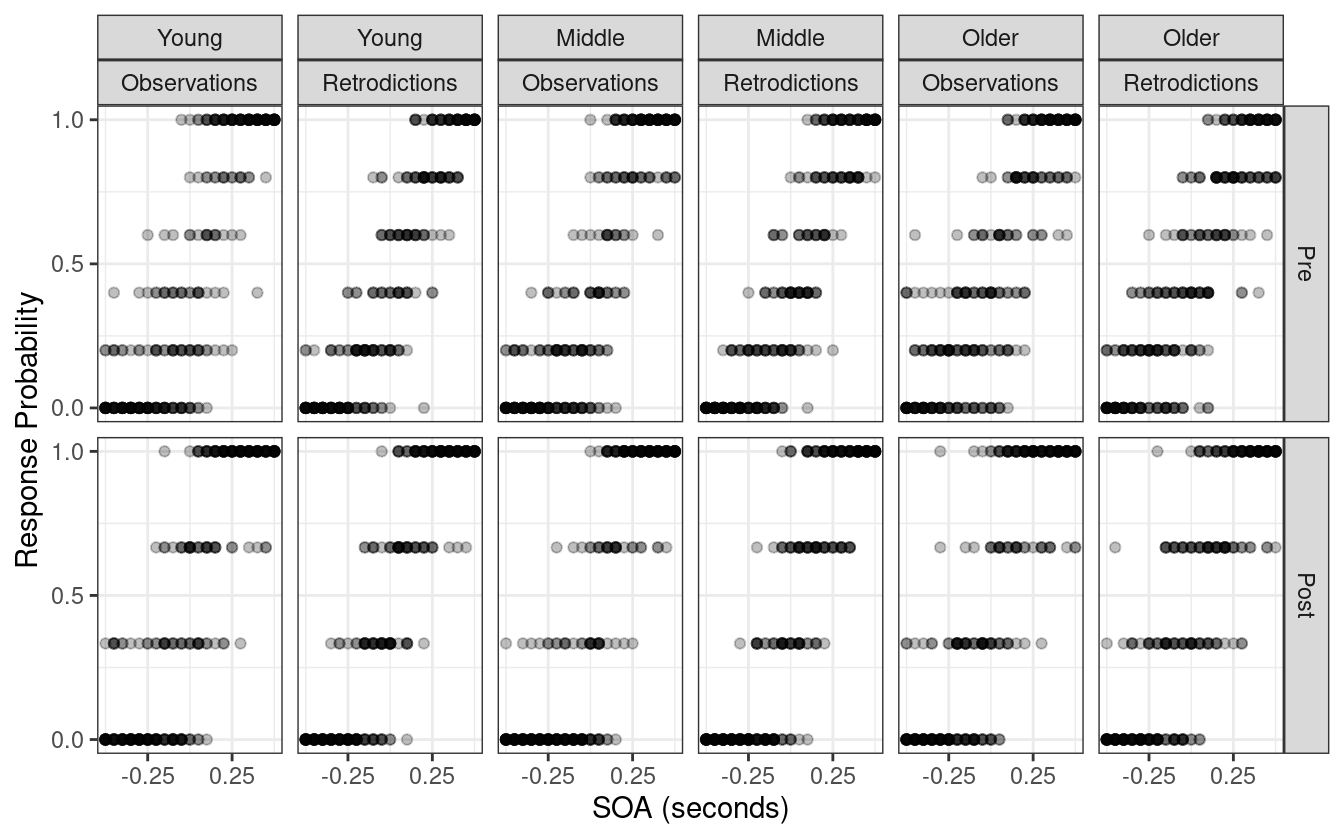
\includegraphics[width=0.85\linewidth]{040-application_files/figure-latex/ch042-obs-vs-retro-plot-1} 

}

\caption{Observed data compared to the posterior retrodictions.}\label{fig:ch042-obs-vs-retro-plot}
\end{figure}

The posterior retrodictions in figure \ref{fig:ch042-obs-vs-retro-plot} show no disagreement between the model and the observed data. This model is almost complete, but has one more problem: it measures the average difference in blocks, and the average difference in age groups, but does not consider any interaction between the two. Implicitly it assumes that temporal recalibration affects all age groups the same which may not be true, so we address this in the next iteration.

\hypertarget{iter3}{%
\section{Iteration 3: adding age-block interaction}\label{iter3}}

There is no change in the pre-model analysis, so we will jump straight to the model development step, after which we will jump right to the posterior retrodictive checks. The changes to the model going forward are minor, and subsequent steps are mostly repetitions of the ones taken in the first two iterations.

\textbf{Post-Model, Pre-Data}

\emph{Develop Model}

We need to model an interaction between age group and treatment. In a simple model in \texttt{R}, interactions between factor variable \(A\) and factor variable \(B\) can be accomplished by taking the cross-product of all the factor levels. For example, if \(A\) has levels \(a, b, c\) and \(B\) has levels \(x, y\), then the interaction variable \(C=A\times B\) will have levels \(ax, ay, bx, by, cx, cy\). The concept is similar in \texttt{Stan}: create a new variable that is indexed by the cross of the two other factor variables.

\begin{equation}
\beta_{G[i] \times trt[i]} \Longrightarrow bGT[G[i], trt[i]]
\label{eq:cross-factor}
\end{equation}

In expression \eqref{eq:cross-factor}, the interaction variable \(\beta_{G[i] \times trt[i]}\) is between age group and treatment. The right hand side is the corresponding \texttt{Stan} parameter. Notice that it is an array-like object that is indexed by the age group at observation \(i\) and the treatment at observation \(i\). For example, observation \(51\) is for a middle age adult subject during the post-adaptation block, so \(bGT[G[51], trt[51]] = bGT[2, 2]\). An interaction term is added for both the slope and intercept in this iteration.

\textbf{Post-Model, Post-Data}

\emph{Diagnose Posterior Fit}

This model has no divergent transitions and no \(\hat{R}\) values greater than \(1.1\). Furthermore the trace-rank plots show uniformity between chains indicating that the chains are all exploring the same regions.

\emph{Posterior Retrodictive Checks}

Because the model now allows for the interaction of age group and block, there is no longer a fixed shift in the posterior distribution of the PSS and JND values. Figure \ref{fig:ch043-posterior-pss-jnd-plot} shows that temporal recalibration had no discernible affect on the PSS estimates for the middle age group.

\begin{figure}

{\centering 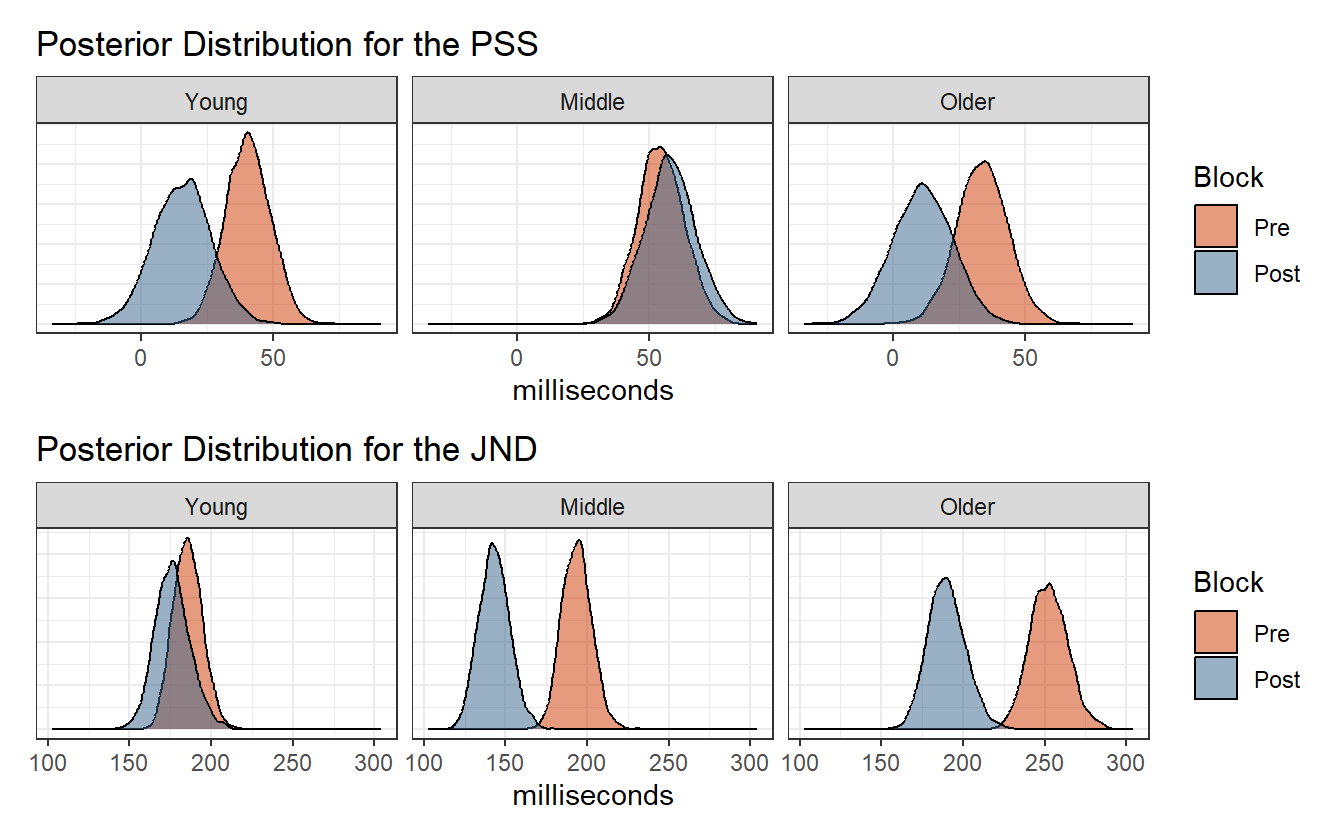
\includegraphics[width=0.85\linewidth]{040-application_files/figure-latex/ch043-posterior-pss-jnd-plot-1} 

}

\caption{Posterior distribution of the PSS and JND.}\label{fig:ch043-posterior-pss-jnd-plot}
\end{figure}

The posterior retrodictions for this model are going to be similar to the last iteration. Instead, we want to see how this model performs when it comes to the posterior retrodictions of the visual TOJ data. There is something peculiar about that data that is readily apparent when we try to fit a GLM using classical MLE.

\setstretch{1.0}

\begin{Shaded}
\begin{Highlighting}[]
\NormalTok{vis\_mle }\OtherTok{\textless{}{-}} \FunctionTok{glm}\NormalTok{(}\FunctionTok{cbind}\NormalTok{(k, n}\SpecialCharTok{{-}}\NormalTok{k) }\SpecialCharTok{\textasciitilde{}} \DecValTok{0} \SpecialCharTok{+}\NormalTok{ sid }\SpecialCharTok{+}\NormalTok{ sid}\SpecialCharTok{:}\NormalTok{soa,}
               \AttributeTok{data =}\NormalTok{ visual\_binomial, }
               \AttributeTok{family =} \FunctionTok{binomial}\NormalTok{(}\StringTok{"logit"}\NormalTok{),}
               \AttributeTok{subset =}\NormalTok{ block }\SpecialCharTok{\%in\%} \FunctionTok{c}\NormalTok{(}\StringTok{"baseline"}\NormalTok{, }\StringTok{"adapt1"}\NormalTok{))}
\end{Highlighting}
\end{Shaded}

\setstretch{2.0}

We get a message saying that the fitted probabilities are numerically 0 or 1. In \ref{glms} we determined that this indicates a large estimate for the slope. This model estimates a slope and an intercept for each subject individually (no pooling), so we can look at the estimates for each subject. Table \ref{tab:ch043-Intensive-Oyster} shows the top 3 coefficients sorted by largest standard error of the estimate for both slope and intercept.

\begin{table}[!h]

\caption{\label{tab:ch043-Intensive-Oyster}Coefficients with the largest standard errors.}
\centering
\begin{tabular}[t]{llrrrr}
\toprule
Subject & Coefficient & Estimate & Std. Error & z value & Pr(>|z|)\\
\midrule
Y-m-CB & Slope & 0.6665 & 25.193 & 0.0265 & 0.9789\\
M-m-BT & Slope & 0.6707 & 24.921 & 0.0269 & 0.9785\\
M-f-DB & Slope & 0.6707 & 24.919 & 0.0269 & 0.9785\\
O-f-MW & Intercept & -3.2427 & 1.235 & -2.6261 & 0.0086\\
Y-f-CJ & Intercept & -2.1336 & 1.024 & -2.0829 & 0.0373\\
\addlinespace
M-f-CC & Intercept & -2.1336 & 1.024 & -2.0829 & 0.0373\\
\bottomrule
\end{tabular}
\end{table}

The standard error of the slope estimate for subject \texttt{Y-m-CB} is incredibly large in comparison to its own estimate and in comparison to the slope with the next largest standard error. Figure \ref{fig:ch043-Y-m-CB-vis-response} shows that there is almost perfect separation in the data for this subject, and that is resulting in a larger slope estimate. In consequence, the estimated JND for this subject is just 3ms which is questionably low.

\begin{figure}

{\centering 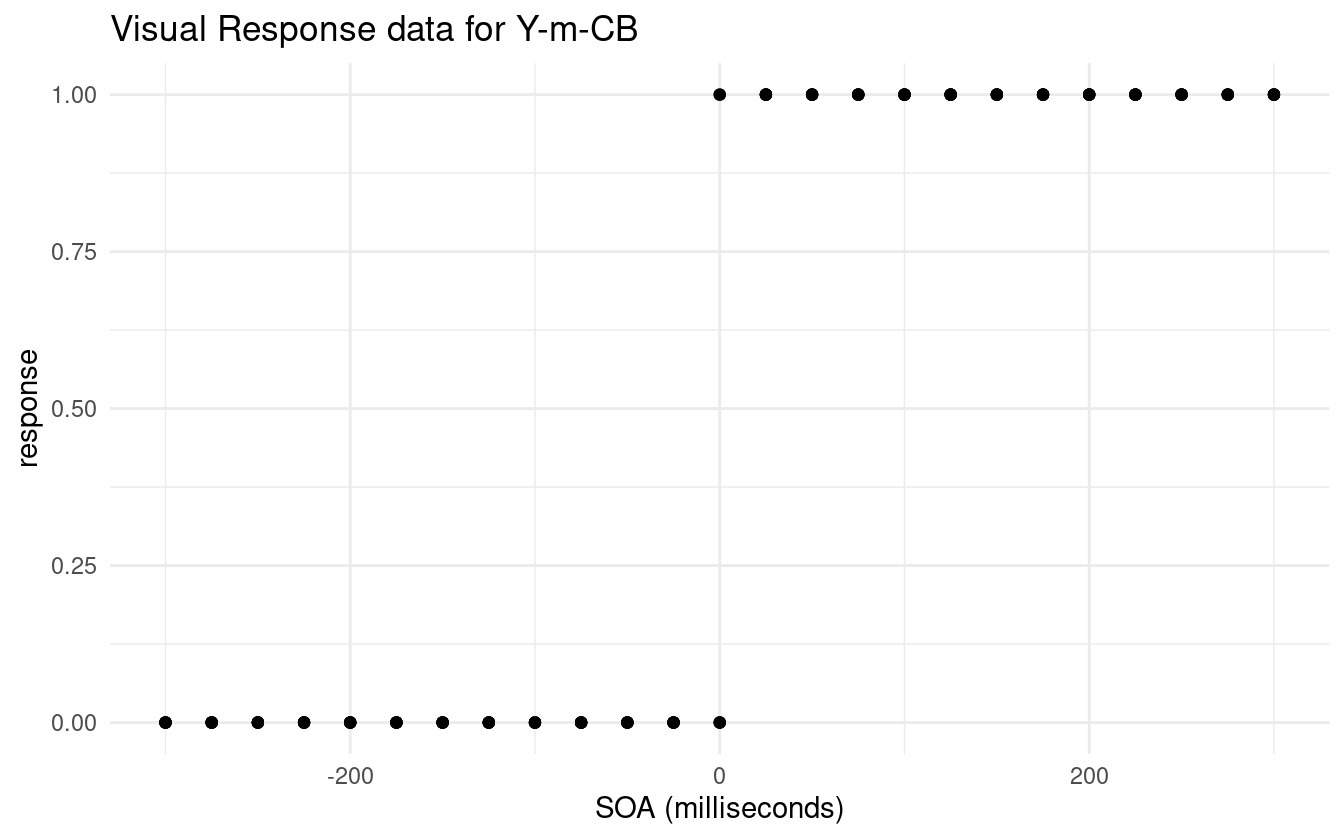
\includegraphics[width=0.85\linewidth]{040-application_files/figure-latex/ch043-Y-m-CB-vis-response-1} 

}

\caption{There is almost complete separation in the data.}\label{fig:ch043-Y-m-CB-vis-response}
\end{figure}

One remedy for this is to pool observations together as we have done for the model in this iteration. The data is pooled together at the age group level and variation in the subjects' responses removes the separation. This isn't always ideal, as sometimes researchers are interested in studying the individuals within the experiment. If accurate inferences about the individual cannot be obtained, then the results are not valid.

Figure \ref{fig:ch043-Iron-Intensive} shows the posterior distribution of psychometric functions for the visual TOJ data. Notice that there is almost no difference between the pre- and post-adaptation blocks.

\begin{figure}

{\centering 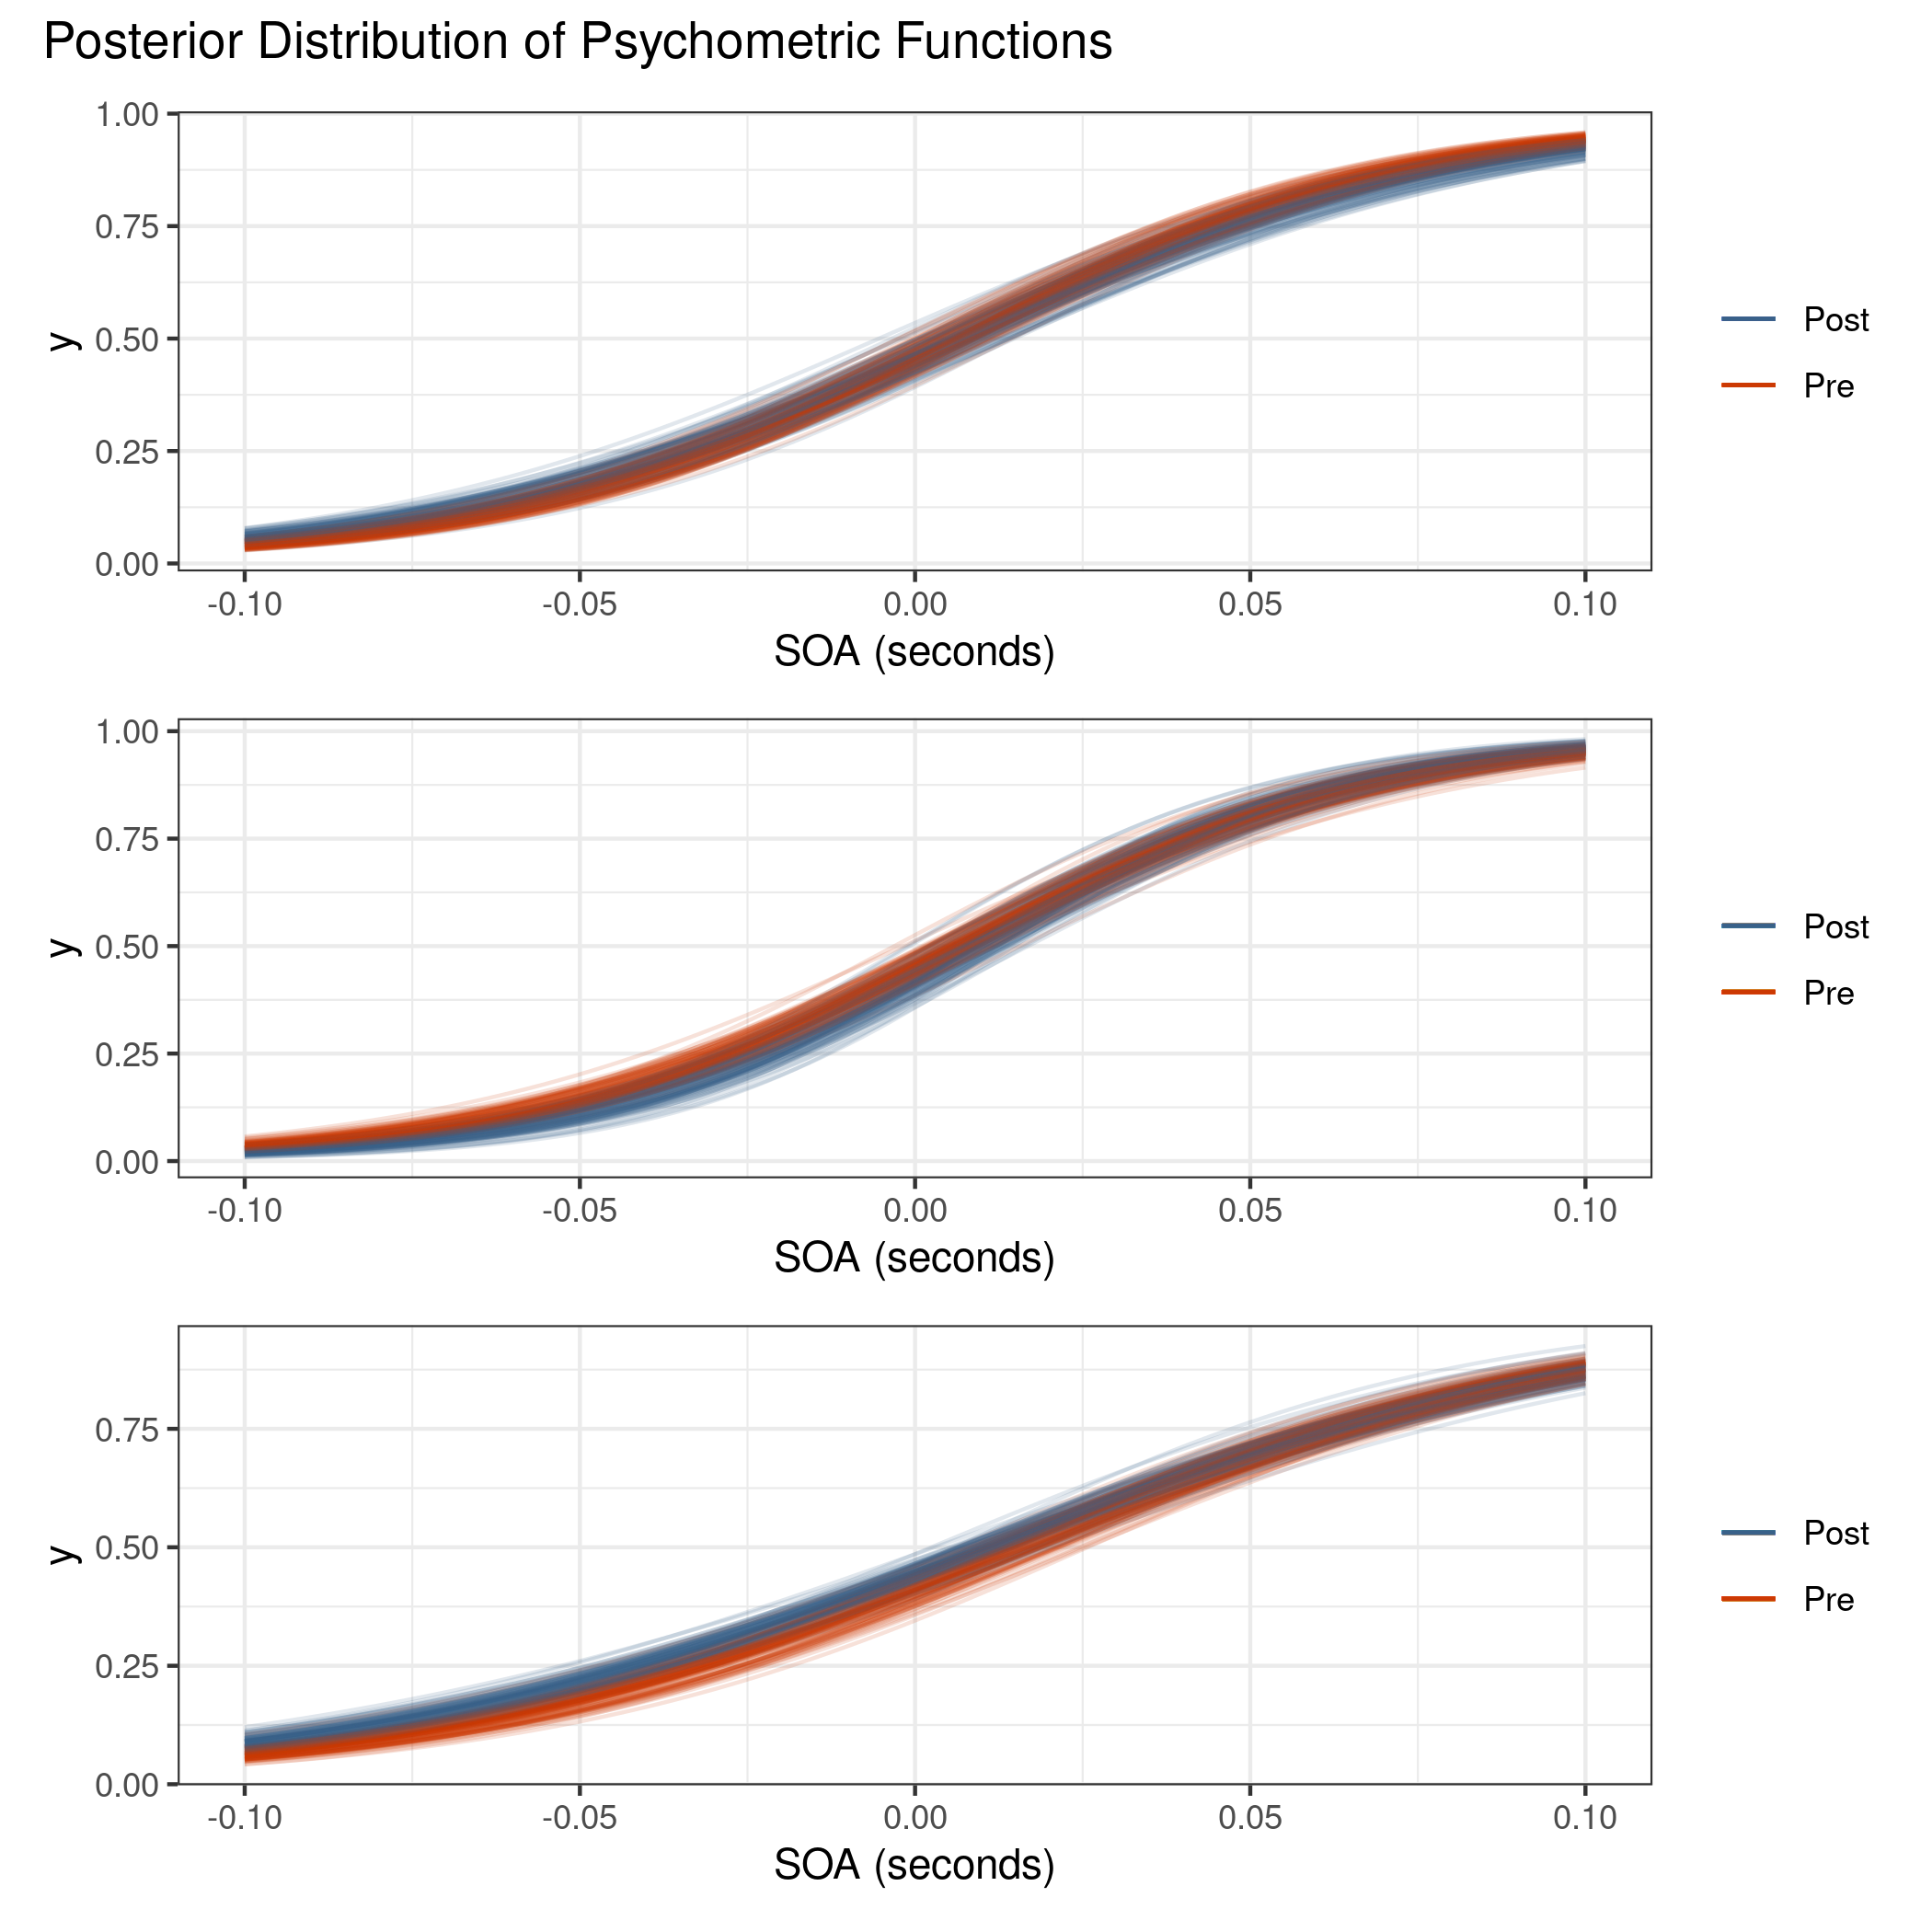
\includegraphics[width=0.85\linewidth]{figures/ch043-Iron-Intensive} 

}

\caption{Posterior distribution of psychometric functions for the visual TOJ data. There is almost no visual difference between the pre- and post-adaptation blocks.}\label{fig:ch043-Iron-Intensive}
\end{figure}

Furthermore, as shown by the posterior retrodictions (figure \ref{fig:ch043-obs-vs-retro-plot}), the model is not fully capturing the variation in the responses near the outer SOA values -- the posterior predictive samples are tight around SOA values near zero.

\begin{figure}

{\centering 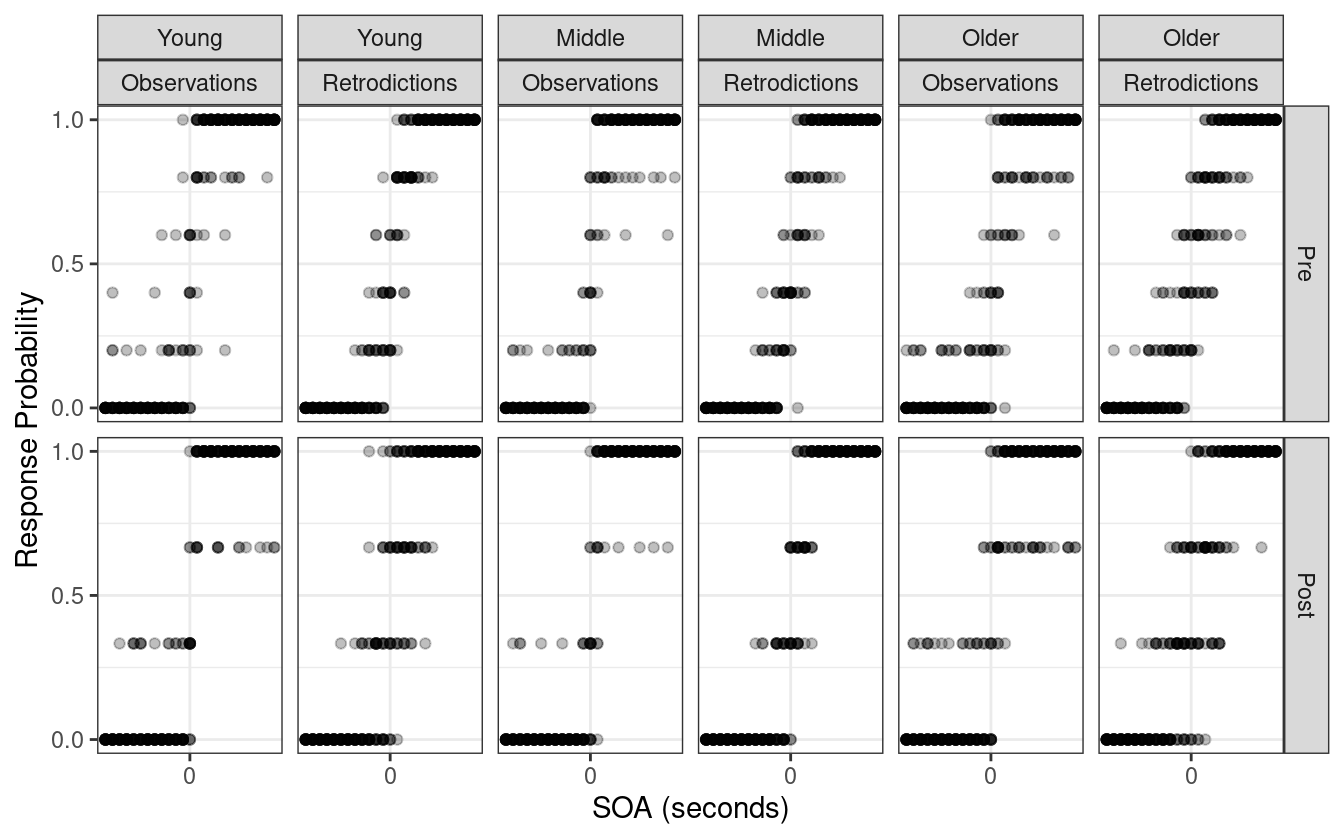
\includegraphics[width=0.85\linewidth]{040-application_files/figure-latex/ch043-obs-vs-retro-plot-1} 

}

\caption{Observed visual TOJ data compared to the posterior retrodictions. The retrodictions are not capturing the variation at the outer SOA values.}\label{fig:ch043-obs-vs-retro-plot}
\end{figure}

Why is the model having difficulty expressing the data? There is one more concept pertaining to psychometric experiments that has been left out until now, and that is a lapse in judgment. Not a lapse in judgment on our part, but the act of a subject having a lapse in judgment while performing an experiment.

\hypertarget{iter4}{%
\section{Iteration 4: adding a lapse rate}\label{iter4}}

\textbf{Pre-Model, Pre-Data}

\emph{Conceptual Analysis}

A lapse in judgment can happen for any reason, and is assumed to be random and independent of other lapses. They can come in the form of the subject accidentally blinking during the presentation of a visual stimulus, or unintentionally pressing the wrong button to respond. Whatever the case is, lapses can have a significant affect on the estimation of the psychometric function.

\textbf{Post-Model, Pre-Data}

\emph{Develop Model}

Lapses can be modeled as occurring independently at some fixed rate. This means that the underlying psychometric function, \(F\), is bounded by some lower and upper lapse rate. This manifests as a scaling and translation of \(F\). For a given lower and upper lapse rate \(\lambda\) and \(\gamma\), the performance function \(\Psi\) is

\[
\Psi(x; \alpha, \beta, \lambda, \gamma) = \lambda + (1 - \lambda - \gamma) F(x; \alpha, \beta)
\]

\begin{figure}

{\centering 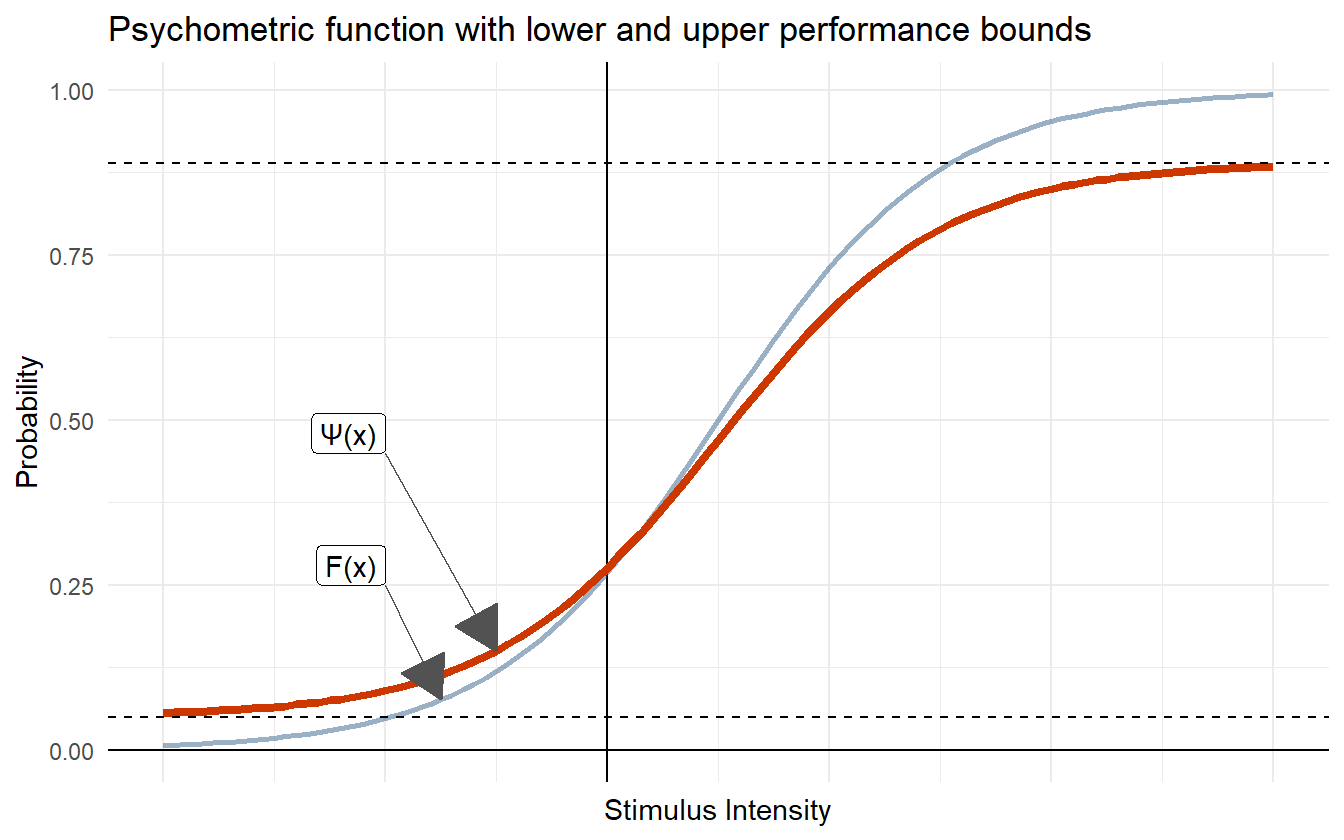
\includegraphics[width=0.85\linewidth]{040-application_files/figure-latex/ch044-plot-pf-with-lapse-1} 

}

\caption{Psychometric function with lower and upper performance bounds.}\label{fig:ch044-plot-pf-with-lapse}
\end{figure}

In certain psychometric experiments, \(\lambda\) is interpreted as the lower performance bound, or the guessing rate. For example, in certain 2-AFC tasks, subjects are asked to respond which of two masses is heavier, and the correctness of their response is recorded. When the masses are the same, the subject can do no better than random guessing. In this task, the lower performance bound is assumed to be 50\% as their guess is split between two choices. As the absolute difference in mass grows, the subject's correctness rate increases, though lapses can still happen. In this scenario, \(\lambda\) is fixed at \(0.5\) and the lapse rate \(\gamma\) is a parameter in the model.

The model we are building for this data does not explicitly record correctness, so we do not give \(\lambda\) the interpretation of a guessing rate. Since the data are recorded as proportion of positive responses, we instead treat \(\lambda\) and \(\gamma\) as lapse rates for negative and positive SOAs. But why should the upper and lower lapse rates be treated separately? A lapse in judgment can occur independently of the SOA, so \(\lambda\) and \(\gamma\) should be the same. With this assumption, we can throw away \(\gamma\) and assume that the lower and upper performance bounds are restricted by the same amount. I.e.

\begin{equation}
  \Psi(x; \alpha, \beta, \lambda) = \lambda + (1 - 2\lambda) F(x; \alpha, \beta)
  \label{eq:Psi}
\end{equation}

While we are including a lapse rate, we will also ask the question of if different age groups have different lapse rates. To answer this (or rather have the model answer this), we include the new parameter \(\lambda_{G[i]}\) into the model so that the lapse rate is estimated for each age group.

It's okay to assume that lapses in judgment are rare, and it's also true that the rate (or probability) of a lapse is bounded in the interval \([0, 1]\). Because of this, we put a \(\mathrm{Beta(4, 96)}\) prior on \(\lambda\) which puts 99\% of the weight below \(0.1\) and an expected lapse rate of \(0.04\).

\emph{Construct Summary Functions}

Since the fundamental structure of the linear model has changed, it is important to update the summary function that computes the distribution of SOA values for a given response probability. Given equation \eqref{eq:Psi}, the summary function \(Q\) is:

\begin{equation}
Q(\pi; \alpha, \beta, \lambda) = \frac{1}{\exp(\beta)} \cdot \mathrm{logit}\left(\frac{\pi - \lambda}{1-2\lambda}\right) + \alpha
\label{eq:Psi-Q}
\end{equation}

\textbf{Post-Model, Post-Data}

\emph{Fit Observed Data}

Because it is the visual data that motivated this iteration, we continue using that data to fit the model and perform posterior retrodictive checks.

\emph{Posterior Retrodictive Checks}

The plot for the distribution of psychometric functions is repeated in figure \ref{fig:ch044-Screaming-Proton}. There is now visual separation between the pre- and post-adaptation blocks, with the latter exhibiting a higher slope, which in turn implies a reduced just noticeable difference which is consistent with the audiovisual data in the previous model.

\begin{figure}

{\centering 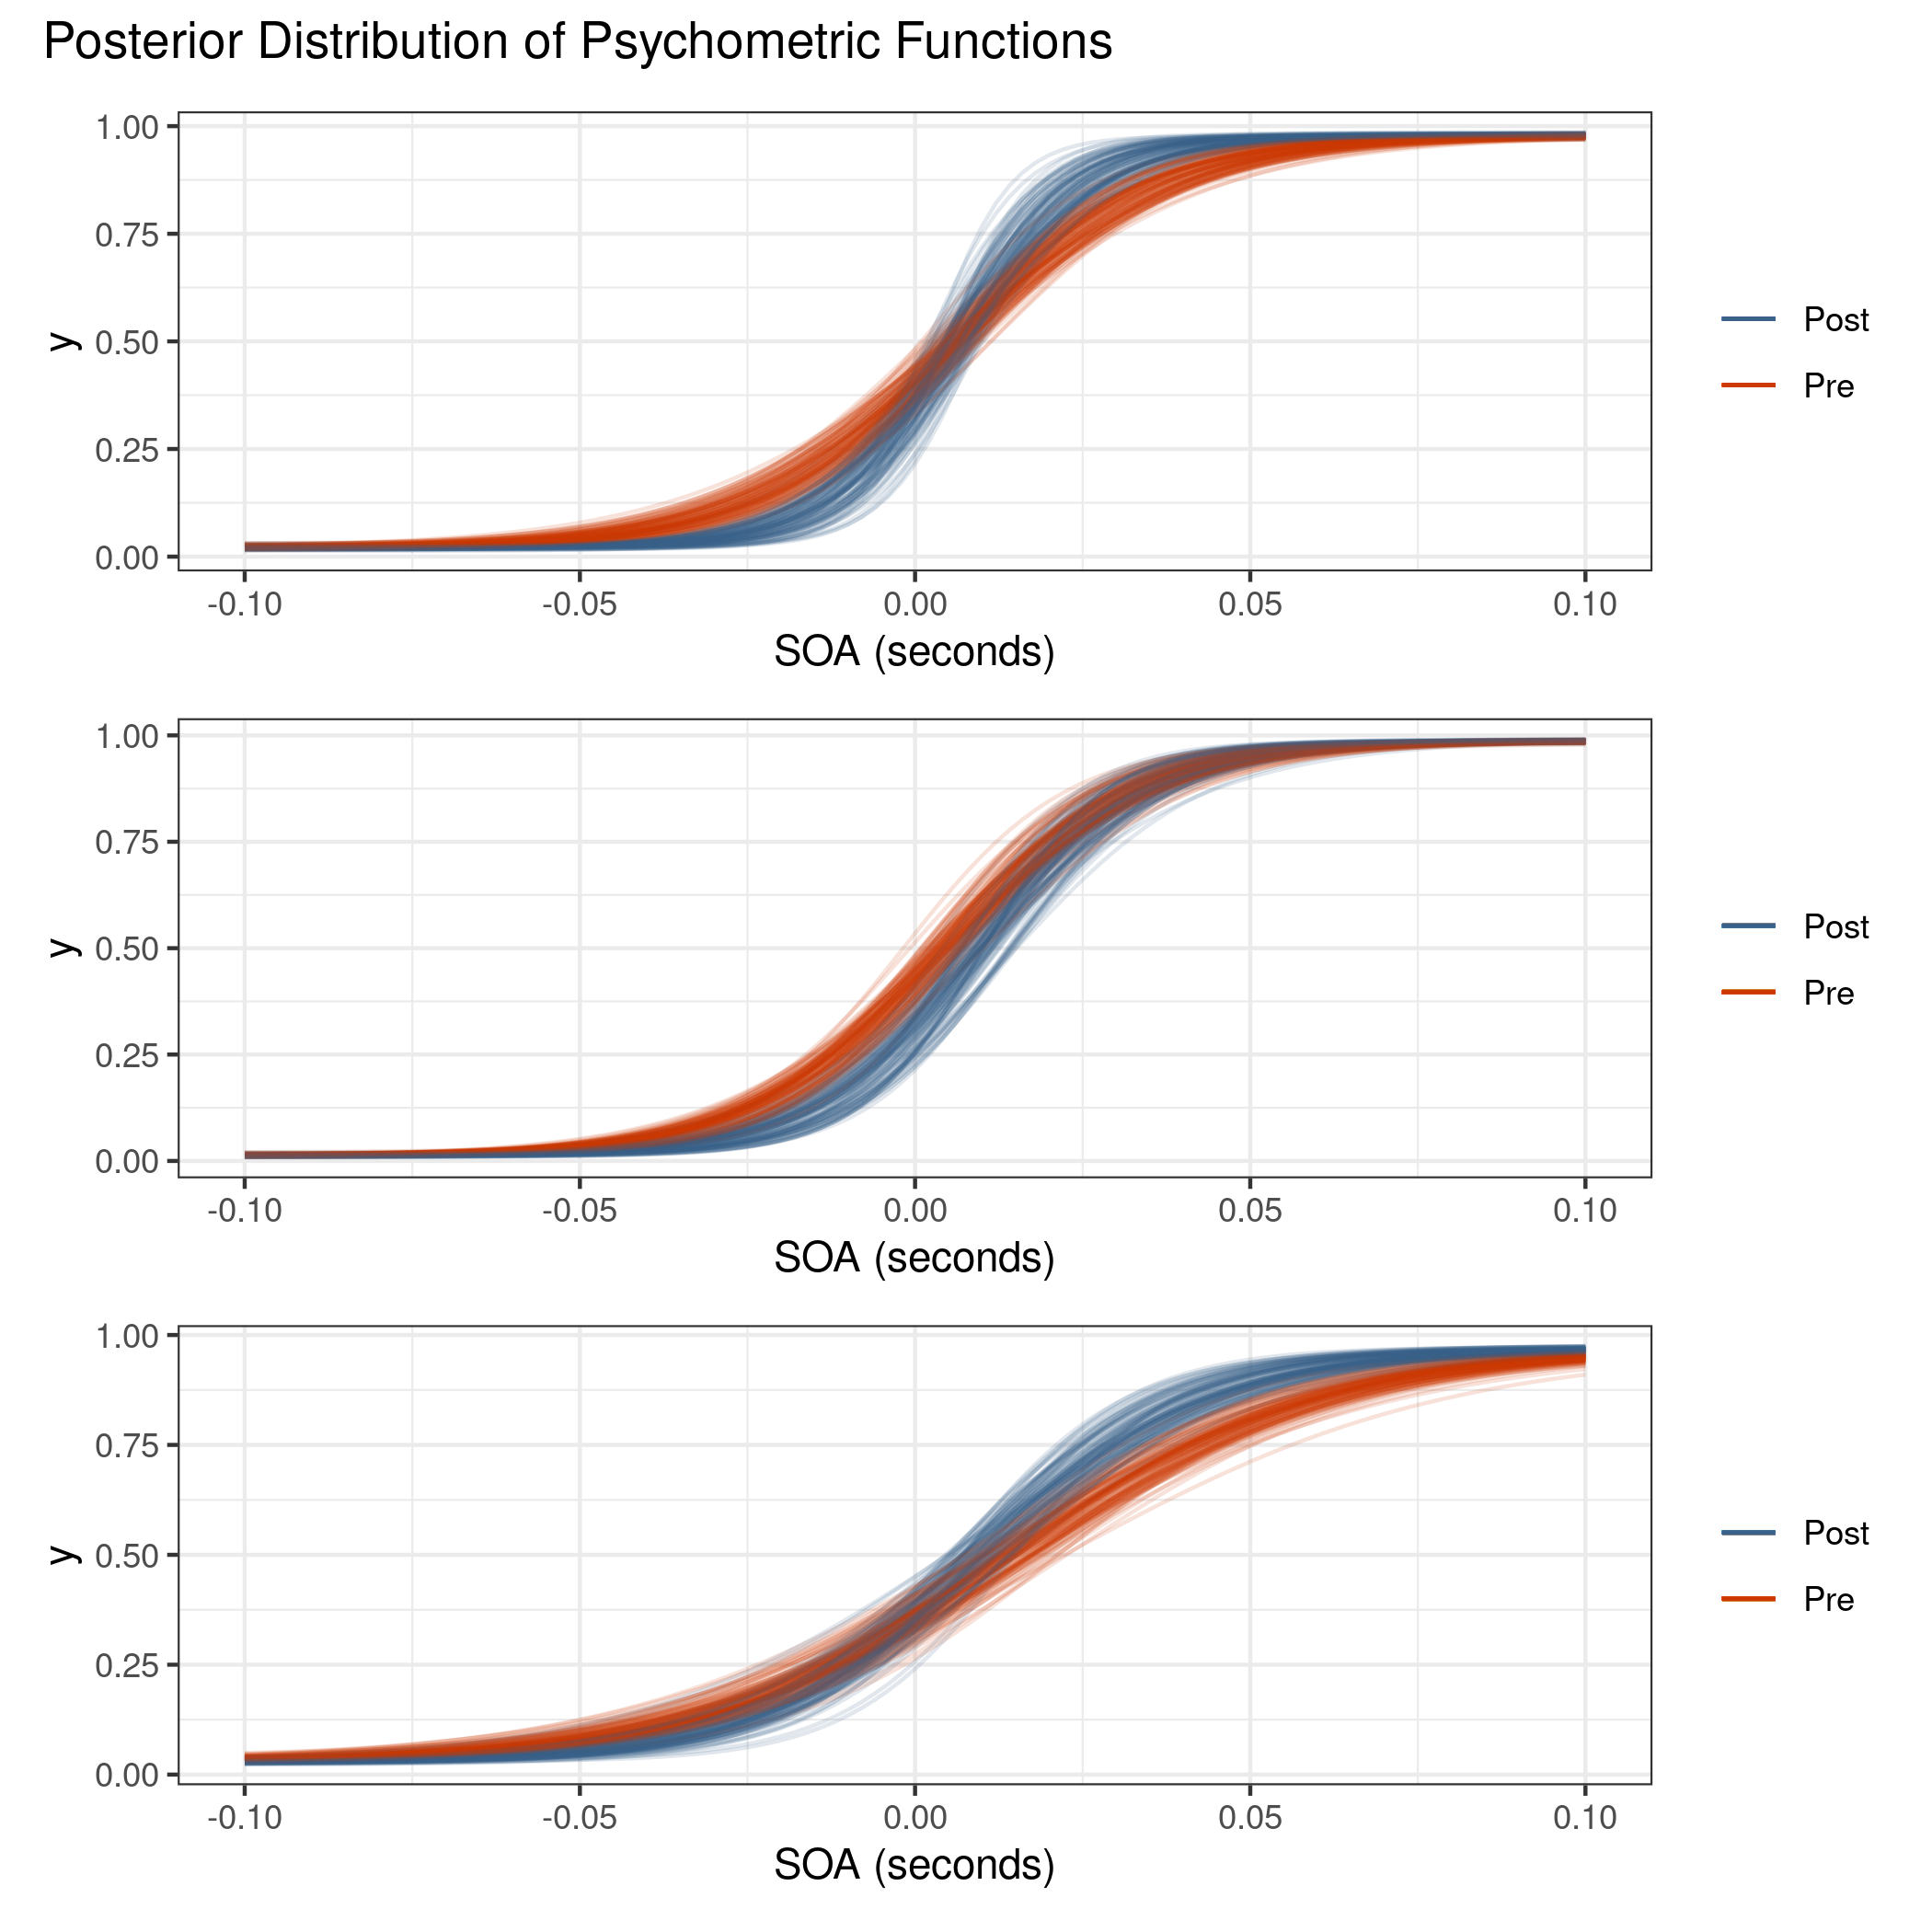
\includegraphics[width=0.85\linewidth]{figures/ch044-Screaming-Proton} 

}

\caption{There is now a visual distinction between the two blocks unlike in the model without lapse rate. The lapse rate acts as a balance between steep slopes near the PSS and variation near the outer SOA values.}\label{fig:ch044-Screaming-Proton}
\end{figure}

The model is now doing better to capture the variation in the outer SOAs. This can best be seen in the comparison of the younger adult pre-adaptation block of figure \ref{fig:ch044-Insane-Metaphor}.

\begin{figure}

{\centering 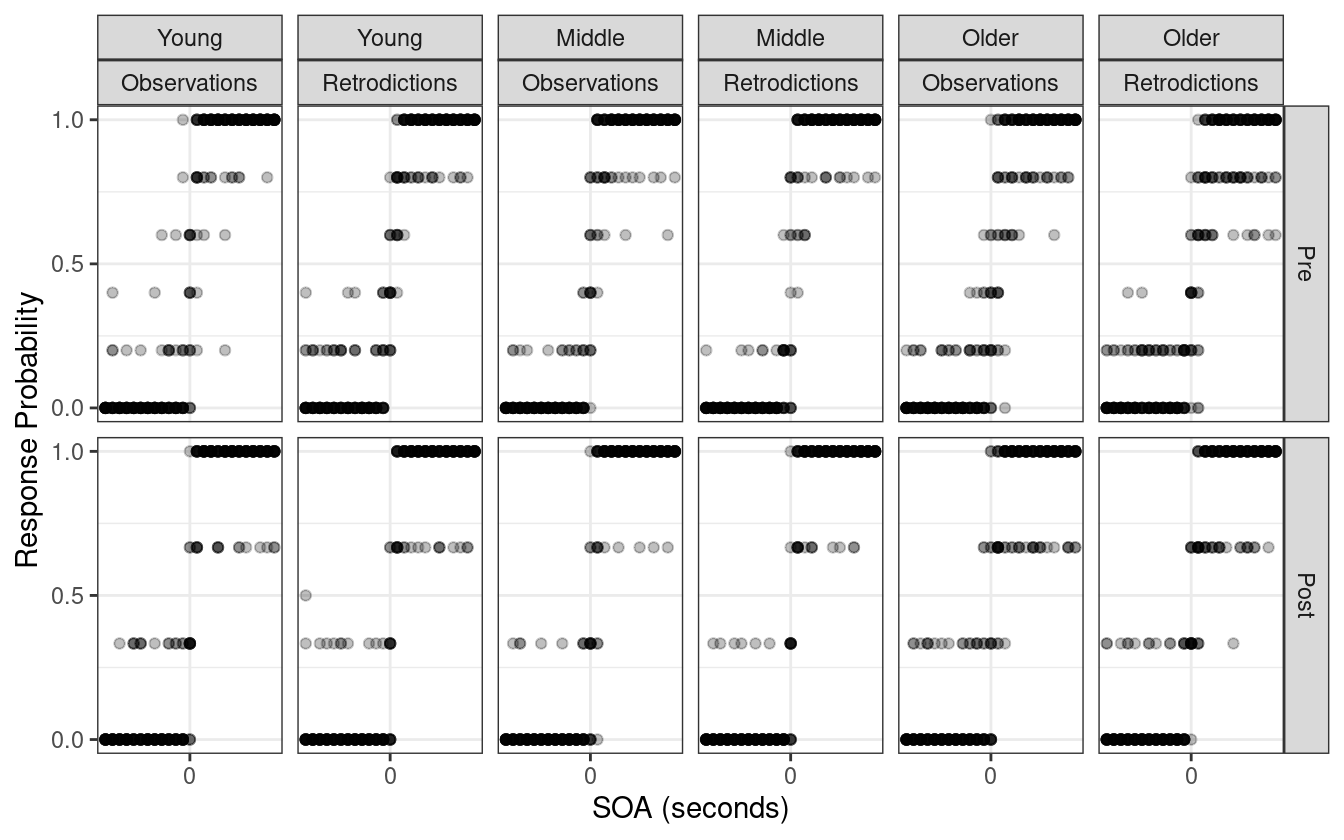
\includegraphics[width=0.85\linewidth]{040-application_files/figure-latex/ch044-Insane-Metaphor-1} 

}

\caption{The lapse rate produces posterior retrodictions that are visually more similar to the observed data than in the previous model, suggesting that the model is now just complex enough to capture the relevant details of the data generating process.}\label{fig:ch044-Insane-Metaphor}
\end{figure}

We can also reintroduce the package \texttt{loo} from the \protect\hyperlink{methods}{chapter 2} to evaluate the predicted predictive performance of the model with lapse rate to the model without the lapse rate as a way of justifying its inclusion. Subjectively the lapse rate model is already doing better, but it is necessary to have quantitative comparisons. Table \ref{tab:ch044-Straw-Epsilon} shows the comparison.

When extracting the PSIS-LOO values, \texttt{loo} warns about some Pareto k diagnostic values that are slightly high:

\setstretch{1.0}

\begin{Shaded}
\begin{Highlighting}[]
\FunctionTok{pareto\_k\_table}\NormalTok{(l044)}
\CommentTok{\#\textgreater{} Pareto k diagnostic values:}
\CommentTok{\#\textgreater{}                          Count Pct.    Min. n\_eff}
\CommentTok{\#\textgreater{} ({-}Inf, 0.5]   (good)     2249  100.0\%  1457      }
\CommentTok{\#\textgreater{}  (0.5, 0.7]   (ok)          1    0.0\%  794       }
\CommentTok{\#\textgreater{}    (0.7, 1]   (bad)         0    0.0\%  \textless{}NA\textgreater{}      }
\CommentTok{\#\textgreater{}    (1, Inf)   (very bad)    0    0.0\%  \textless{}NA\textgreater{}      }
\CommentTok{\#\textgreater{} }
\CommentTok{\#\textgreater{} All Pareto k estimates are ok (k \textless{} 0.7).}
\end{Highlighting}
\end{Shaded}

\setstretch{2.0}

There is one observation in the data set that has a \(k\) value between \(0.5\) and \(0.7\). This means that the estimated Pareto distribution used for smoothing has infinite variance, but practically it is still usable for estimating predictive performance.

\begin{table}[!h]

\caption{\label{tab:ch044-Straw-Epsilon}Model without lapse rate compared to one with lapse rate.}
\centering
\begin{tabular}[t]{lrrrrr}
\toprule
Model & elpd\_diff & se\_diff & elpd\_loo & p\_loo & se\_p\_loo\\
\midrule
Lapse & 0.0 & 0.00 & -1001 & 19.22 & 1.902\\
No Lapse & -259.4 & 31.92 & -1260 & 23.10 & 2.259\\
\bottomrule
\end{tabular}
\end{table}

The model with the lapse rates has higher estimated predicted performance than the model without lapse rates as measured by the ELPD. We can now perform one last iteration of the model by including the subject level estimates. Even though we're only interested in making inferences at the group level, including the subject level might improve predictive performance.

\hypertarget{iter5}{%
\section{Iteration 5: adding subjects}\label{iter5}}

The only change in this iteration is the addition of the subject level parameters for the slope and intercept. The model is:

\setstretch{1.0}

\begin{equation}
\begin{split}
k_i &\sim \mathrm{Binomial}(n_i, p_i) \\
p_i &= \lambda_{G[i]} + (1 - 2\lambda_{G[i]})\exp(\mu_\beta) (x_i - \mu_\alpha) \\
\mu_\alpha &= \alpha + \alpha_{G[i], trt[i]} + \alpha_{S[i]} \\
\mu_\beta &= \beta + \beta_{G[i], trt[i]} + \beta_{S[i]} \\
\lambda_{G} &\sim \mathrm{Beta}(4, 96) \\
\hat{\alpha}, \hat{\alpha}_{G\times trt}, \hat{\alpha}_{S} &\sim \mathcal{N}(0, 1^2) \\
\hat{\beta}, \hat{\beta}_{G\times trt}, \hat{\beta}_{S} &\sim \mathcal{N}(0, 1^2) \\
\hat{\sigma}_{G\times trt}, \hat{\gamma}_{G\times trt}, \hat{\tau}_{S}, \hat{\nu}_{S} &\sim \mathcal{U}(0, \pi/2) \\
\alpha &= 0.06 \cdot \hat{\alpha} \\
\alpha_{G\times trt} &= \sigma_{G\times trt} \cdot \hat{\alpha}_{trt} \\
\alpha_{S} &= \tau_{S} \cdot \hat{\alpha}_{S} \\
\sigma_{G \times trt} &= \tan(\hat{\sigma}_{G \times trt}) \\
\tau_{S} &= \tan(\hat{\tau}_{S}) \\
\beta &= 3 + 1 \cdot \hat{\beta} \\
\beta_{G\times trt} &= \gamma_{G\times trt} \cdot \hat{\beta}_{G\times trt} \\
\beta_{S} &= \nu_{S} \cdot \hat{\beta}_{S} \\
\gamma_{G\times trt} &= \tan(\hat{\gamma}_{G\times trt}) \\
\nu_{S} &= \tan(\hat{\nu}_{S})
\end{split}
\label{eq:iter5-model}
\end{equation}
\setstretch{2.0}

\textbf{Post-Model, Post-Data}

\emph{Diagnose Posterior Fit}

There is only one divergent transition for this model indicating no issues with the algorithmic configuration. Checking the trace plot for the multilevel variance terms also indicates no problems with the sampling.

\begin{figure}

{\centering 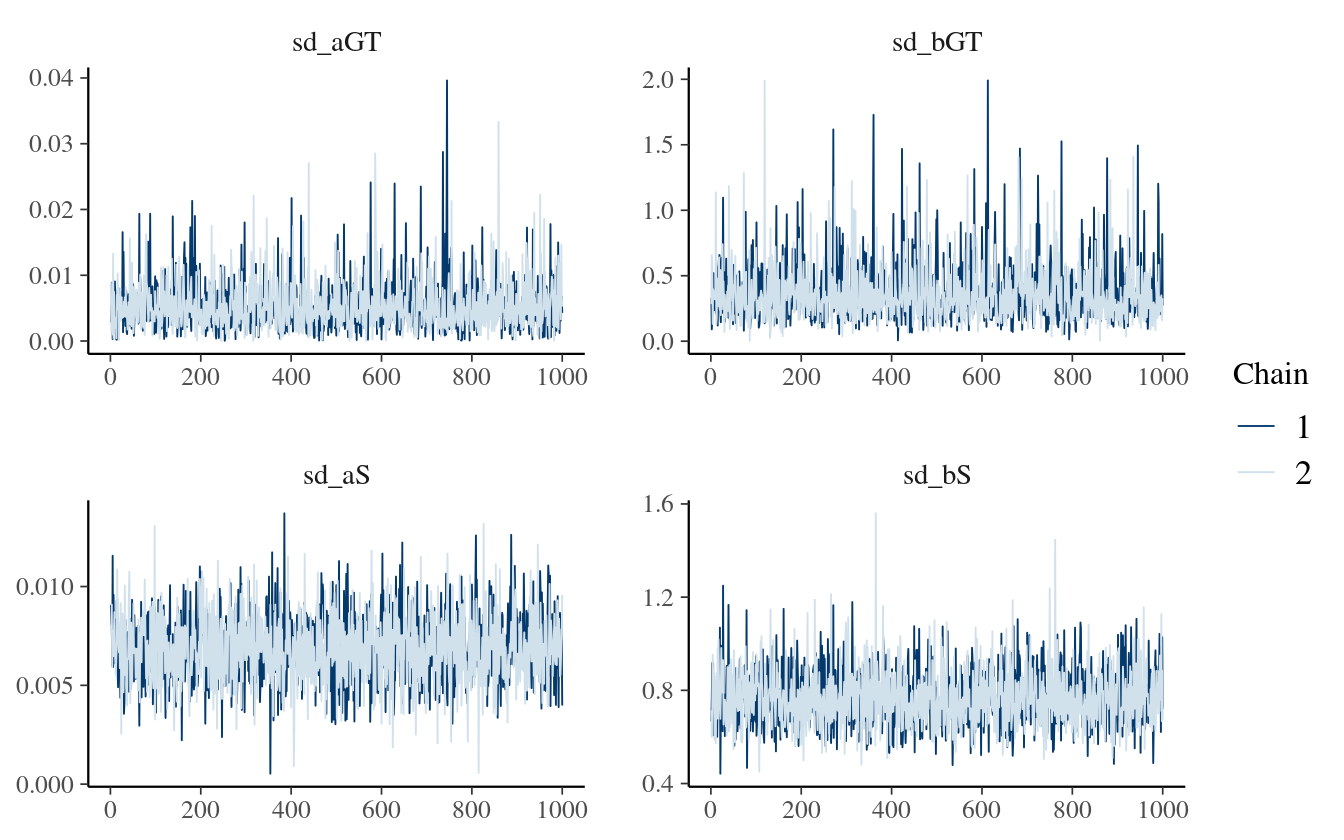
\includegraphics[width=0.85\linewidth]{040-application_files/figure-latex/ch045-Mysterious-Neptune-1} 

}

\caption{The multilevel model with lapse and subject-level terms fits efficiently with no issues.}\label{fig:ch045-Mysterious-Neptune}
\end{figure}

This model also utilizes thinning while fitting for data saving reasons. As such the autocorrelation between samples is reduced and the model achieves a high \(N_{\mathrm{eff}}/N\) ratio (figure \ref{fig:ch045-Nocturnal-Temple}).

\begin{figure}

{\centering 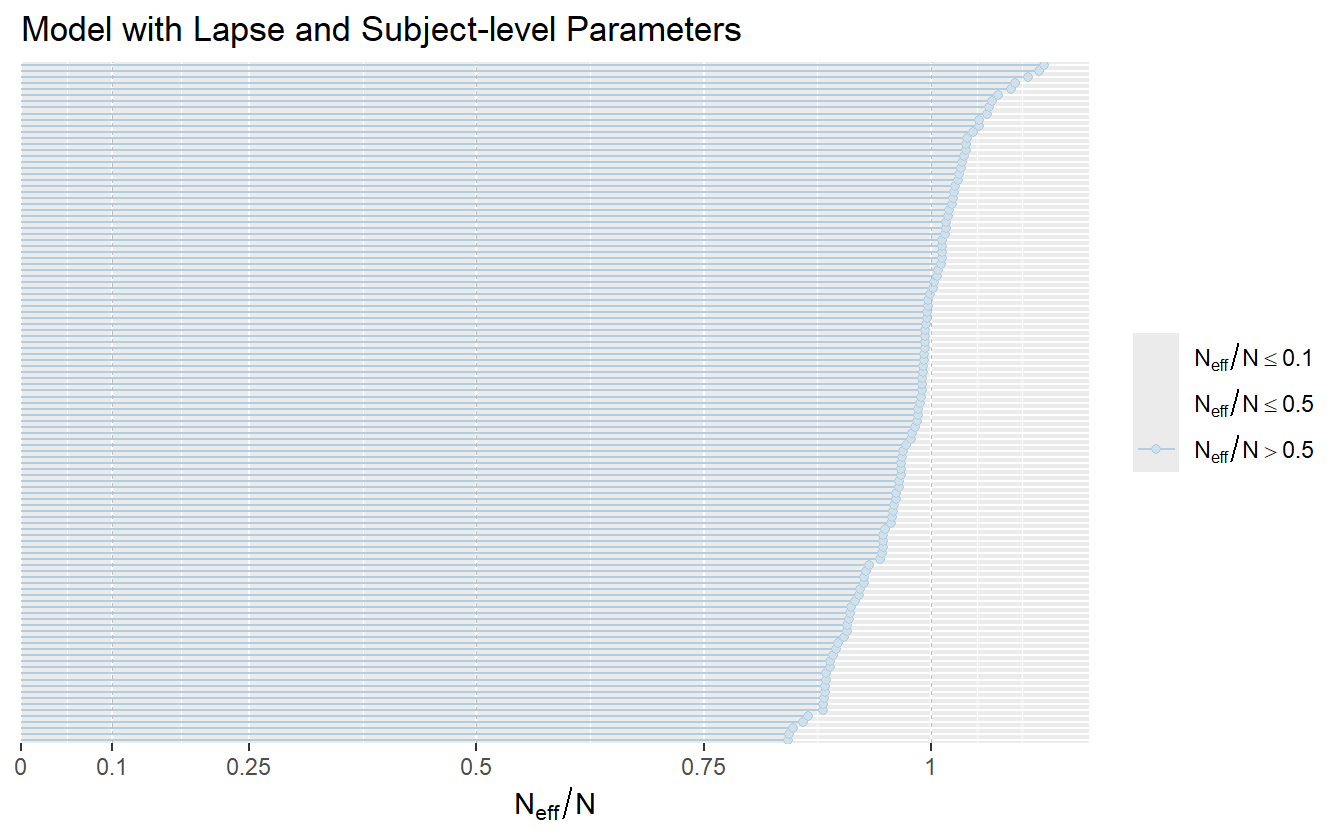
\includegraphics[width=0.85\linewidth]{040-application_files/figure-latex/ch045-Nocturnal-Temple-1} 

}

\caption{The model with lapse rates and subject-level parameters achieves a sampling efficiency partially due to thinning.}\label{fig:ch045-Nocturnal-Temple}
\end{figure}

\emph{Posterior Predictive Comparison}

In lieu of posterior retrodictions (which would appear similar to those of the last iteration), we compare the model with subject-level parameters to the one without. There are a handful of observations in the subject-level model that have a Pareto \(k\) value higher than \(0.7\) which indicates impractical convergence rates and unreliable Monte Carlo error estimates. For more accurate estimation of predictive performance, \(k\)-fold CV or LOOCV is recommended.

\setstretch{1.0}

\begin{verbatim}
#> Pareto k diagnostic values:
#>                          Count Pct.    Min. n_eff
#> (-Inf, 0.5]   (good)     2182  97.0%   320       
#>  (0.5, 0.7]   (ok)         52   2.3%   166       
#>    (0.7, 1]   (bad)        16   0.7%   46        
#>    (1, Inf)   (very bad)    0   0.0%   <NA>
\end{verbatim}

\setstretch{2.0}

\begin{table}[!h]

\caption{\label{tab:ch045-Deserted-Fish}Model without subjects compared to one with subjects.}
\centering
\begin{tabular}[t]{lrrrrr}
\toprule
Model & elpd\_diff & se\_diff & elpd\_loo & p\_loo & se\_p\_loo\\
\midrule
With Subjects & 0.00 & 0.00 & -924.4 & 75.04 & 5.402\\
Without Subjects & -76.75 & 19.29 & -1001.1 & 19.22 & 1.902\\
\bottomrule
\end{tabular}
\end{table}

Including the subject-level information significantly improves the ELPD, and even though there are over 100 parameters in the model (slope and intercept for each of the 45 subjects), the effective number of parameters is much less. Since this new model is capable of making inferences at both the age group level and the subject level, we use it for drawing inferences in the results chapter.

\hypertarget{results}{%
\chapter{Psychometric Results}\label{results}}

What was the point of going through all the work of building a model if not to answer the questions that motivated the model in the first place? To reiterate, the questions pertain to how the brain reconciles stimuli originating from different sources, and if biological (age) and contextual (task, temporal recalibration) factors contribute to global percepts. The way through which these questions are answered is through a psychometric experiment and the resulting psychometric function (\protect\hyperlink{data}{chapter 3}). This chapter is divided into three sections: the affects of temporal recalibration on perceptual synchrony, the affects of temporal recalibration on temporal sensitivity, and the consideration of a lapse rate. Also recall that there are four separate tasks - audiovisual, visual, duration, and sensorimotor.

Temporal recalibration consists of presenting a subject with an adapting stimulus throughout a block of a psychometric experiment. Depending on the mechanisms at work, the resulting psychometric function can either be shifted (biased) towards the adapting stimulus (lag adaption) or away (Bayesian adaptation). The theory of integrating sensory signals is beyond the scope of this paper, but some papers discussing sensory adaptation in more detail are \citet{miyazaki2006bayesian}, \citet{sato2011bayesian}, and \citet{stocker2005sensory}. The statistical associations are reported without consideration for the deeper psychological theory.

\hypertarget{on-perceptual-synchrony}{%
\section{On Perceptual Synchrony}\label{on-perceptual-synchrony}}

Perceptual synchrony is when the temporal delay between two stimuli is small enough so that the brain integrates the two signals into a global percept - perceived as happening simultaneously. Perceptual synchrony is studied through the point of subjective simultaneity (PSS), and in a simple sense represents the bias towards a given stimulus. Ideally the bias would be zero, but human perception is liable to change due to every day experiences. The pre-adaptation block is a proxy for implicit bias, and the post-adaptation indicates whether lag or Bayesian adaptation is taking place. Some researchers believe that both forms of adaptation are taking place at all times and that the mixture rates are determined by biological and contextual factors. We try to stay away from making any strong determinations and will only present the results conditional on the model and the data.

\textbf{Audiovisual TOJ Task}

There are two ways that we can visually draw inferences across the six different age-block combinations. The distributions can either be faceted by age group, or they can be faceted by block. There are actually many ways that the data can be presented, but these two methods of juxtaposition help to answer two questions - how does the effect of adaptation vary by age group, and is there a difference in age groups by block? The left hand plot of figure \ref{fig:ch050-Eastern-Cat} answers the former, and the right hand plot answers the latter.

\begin{figure}

{\centering 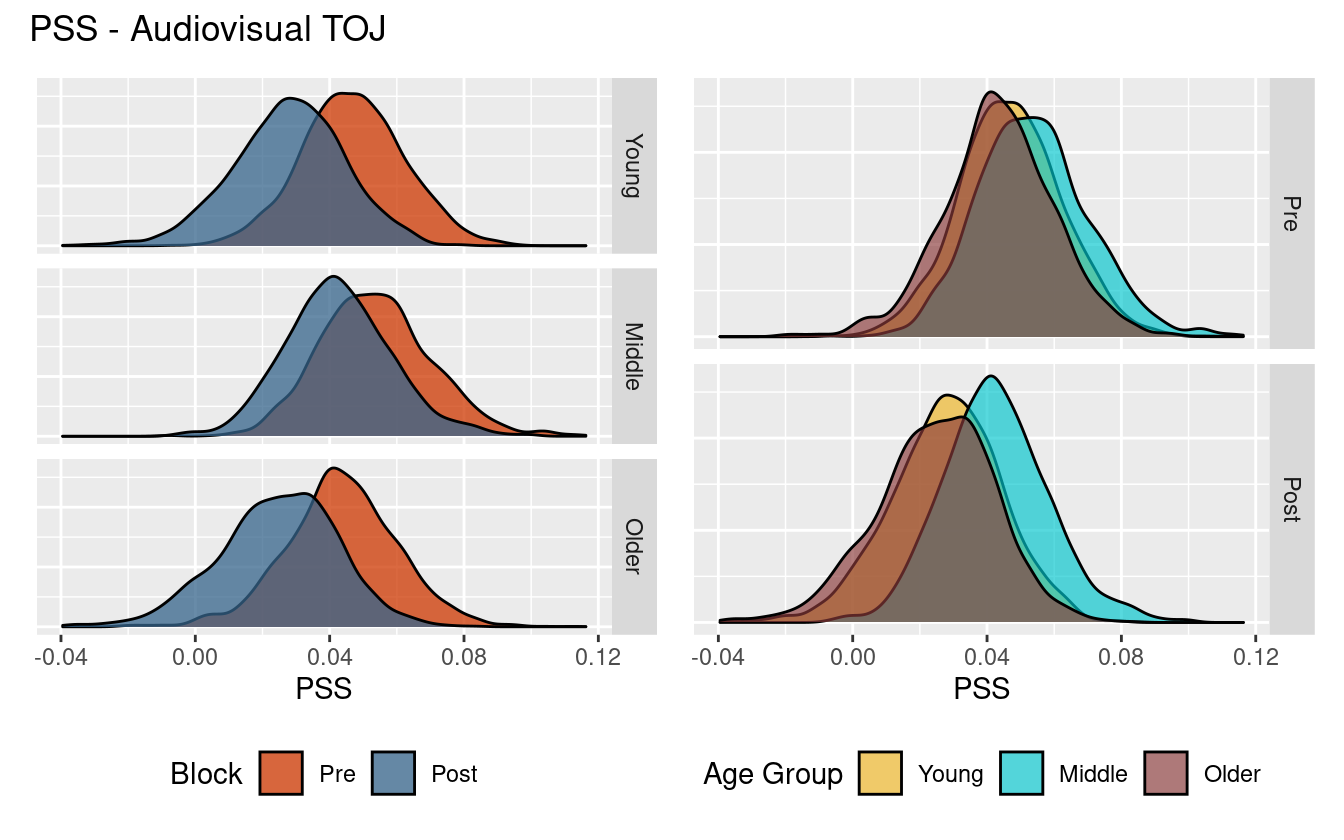
\includegraphics[width=0.85\linewidth]{050-results_files/figure-latex/ch050-Eastern-Cat-1} 

}

\caption{Posterior distribution of PSS values for the audiovisual task.}\label{fig:ch050-Eastern-Cat}
\end{figure}

Across all age groups, temporal recalibration results in a negative shift towards zero in the PSS (as shown by the left hand plot), but there is no significant difference in the PSS between age groups (right hand plot). A very convenient consequence of using MCMC is that the samples from the posterior can be recombined in many ways to describe new phenomena. The PSS values can even be pooled across age groups so that the marginal affect of recalibration may be considered (left hand plot of figure \ref{fig:ch050-Beta-Lonesome}).

\begin{figure}

{\centering 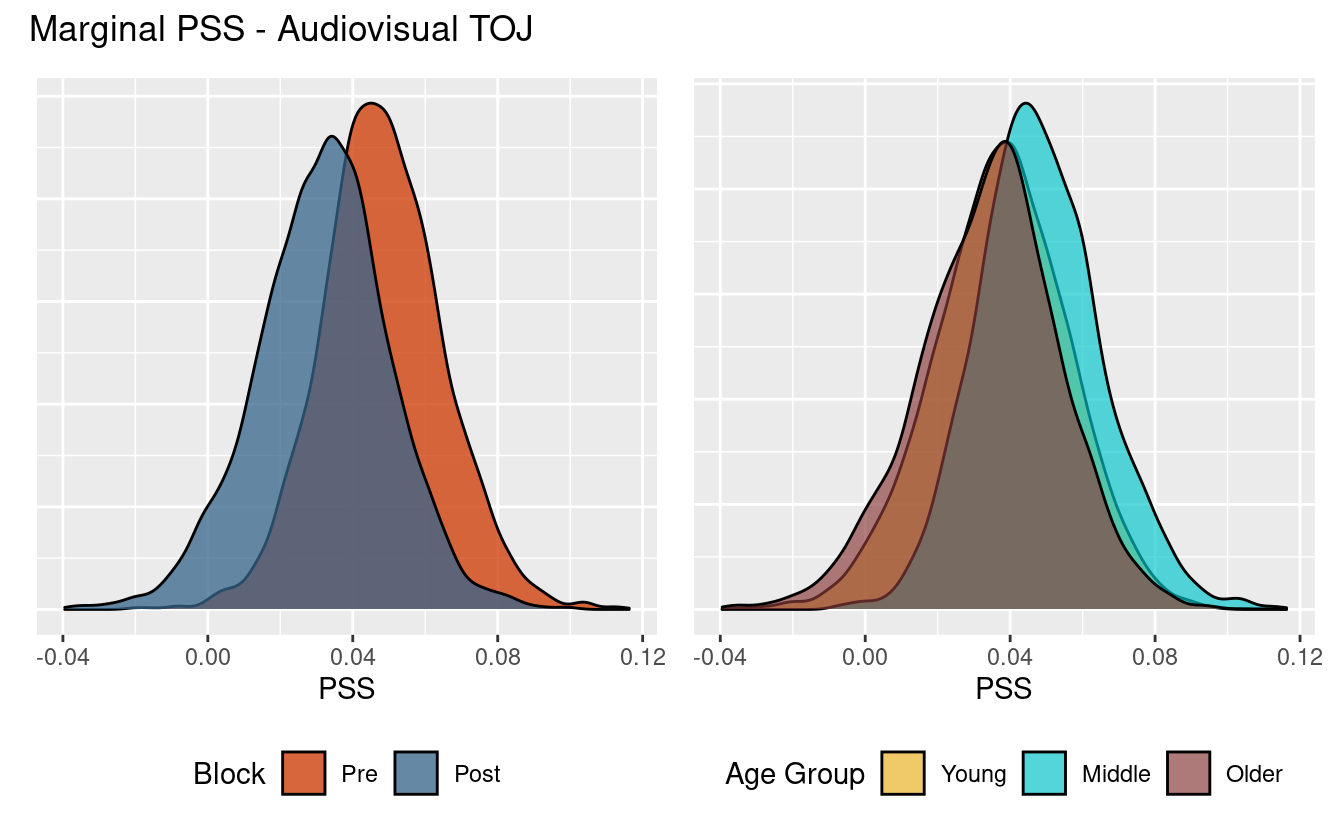
\includegraphics[width=0.85\linewidth]{050-results_files/figure-latex/ch050-Beta-Lonesome-1} 

}

\caption{Posterior distribution of PSS values for the audiovisual task. Left: Marginal over age group. Right: Marginal over block.}\label{fig:ch050-Beta-Lonesome}
\end{figure}

Now with the marginal of age group, the distribution of differences between pre- and post-adaptation blocks can be calculated. We could report a simple credible interval, but it almost seems disingenuous given that the entire distribution is available. We could report that the \(90\%\) highest posterior density interval (HPDI) of the difference is \((-0.037, 0.002)\), but consider the following figure instead (figure \ref{fig:ch050-Omega-Permanent}).

\begin{figure}

{\centering 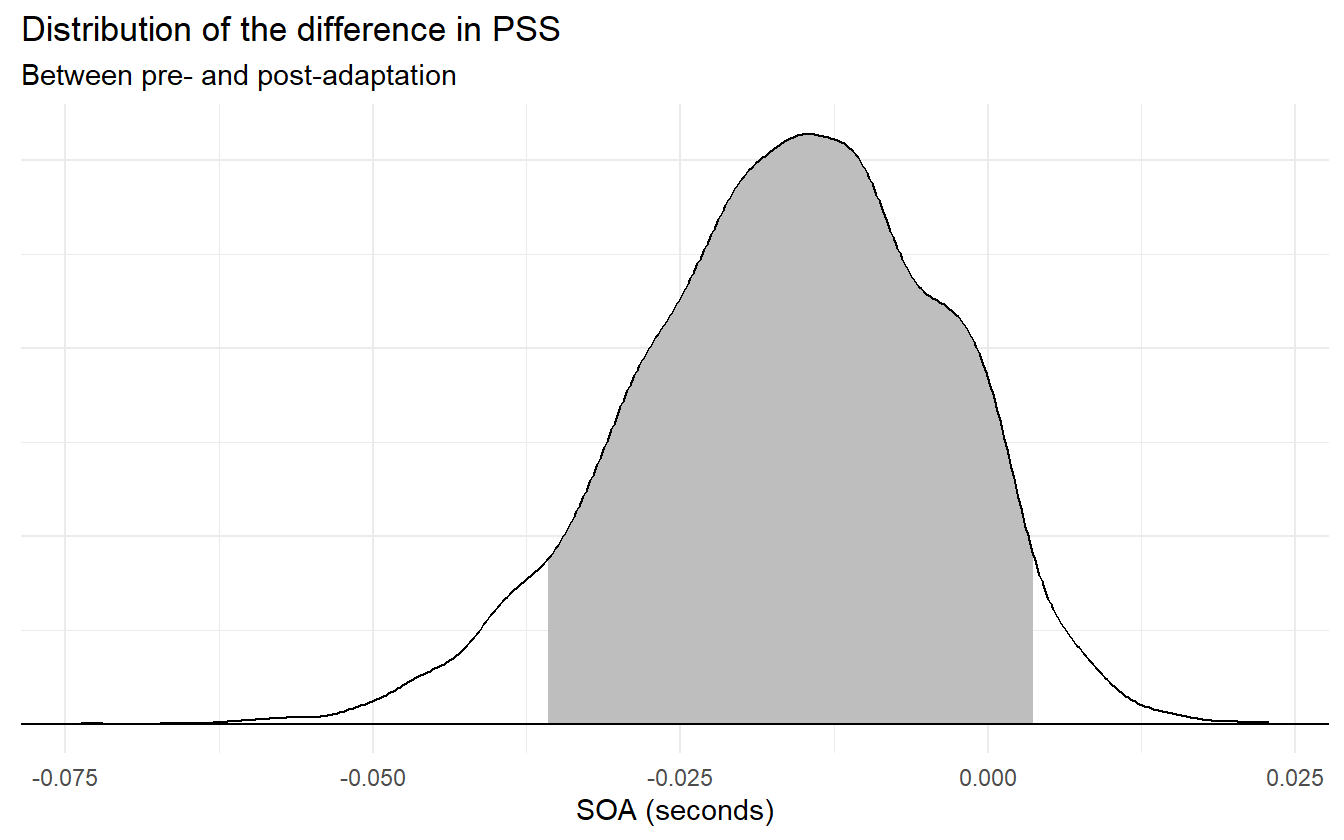
\includegraphics[width=0.85\linewidth]{050-results_files/figure-latex/ch050-Omega-Permanent-1} 

}

\caption{Distribution of differences for pre- and post-adaptation PSS values with 90\% HPDI.}\label{fig:ch050-Omega-Permanent}
\end{figure}

Figure \ref{fig:ch050-Omega-Permanent} shows the distribution of differences with the \(90\%\) HPDI region shaded. From this figure, one might conclude that the effect of recalibration, while small, is still noticeable for the audiovisual task. While this could be done for every task in the rest of this chapter, it is not worth repeating as we are not trying to prove anything about the psychometric experiment itself (that is for a later paper). The point of this demonstration is simply that it can be done (and easily), and how to summarize the data both visually and quantitatively.

\textbf{Visual TOJ Task}

\begin{figure}

{\centering 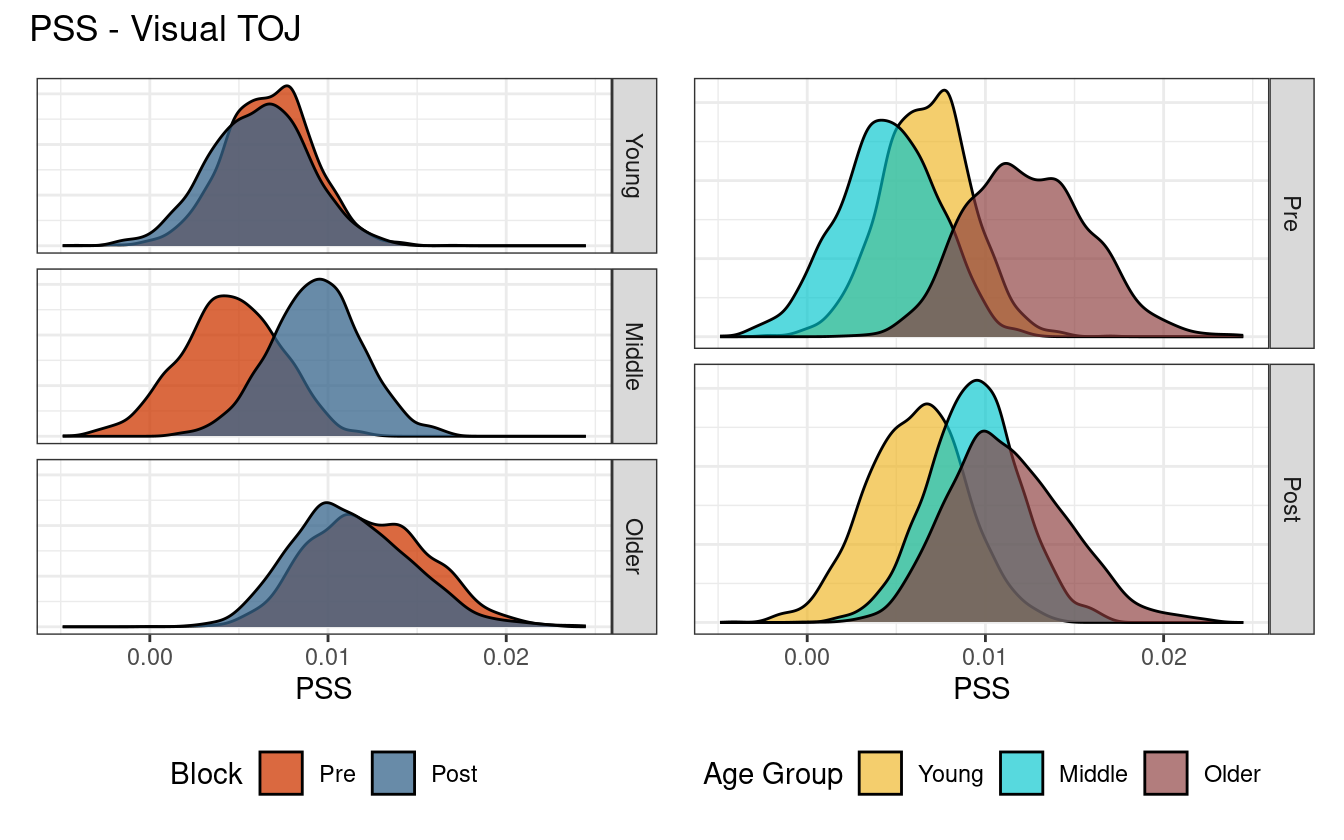
\includegraphics[width=0.85\linewidth]{050-results_files/figure-latex/ch050-Gruesome-Waffle-1} 

}

\caption{Posterior distribution of PSS values for the visual task.}\label{fig:ch050-Gruesome-Waffle}
\end{figure}

Here there is no clear determination if recalibration has an effect on perceptual synchrony, as it is only the middle age group that shows a shift in bias. Even more, there is a lot of overlap between age group. Looking at the marginal distributions (figure \ref{fig:ch050-Cold-Gamma}), there may be a difference between the younger and older age groups, and the middle age and older age groups.

\begin{figure}

{\centering 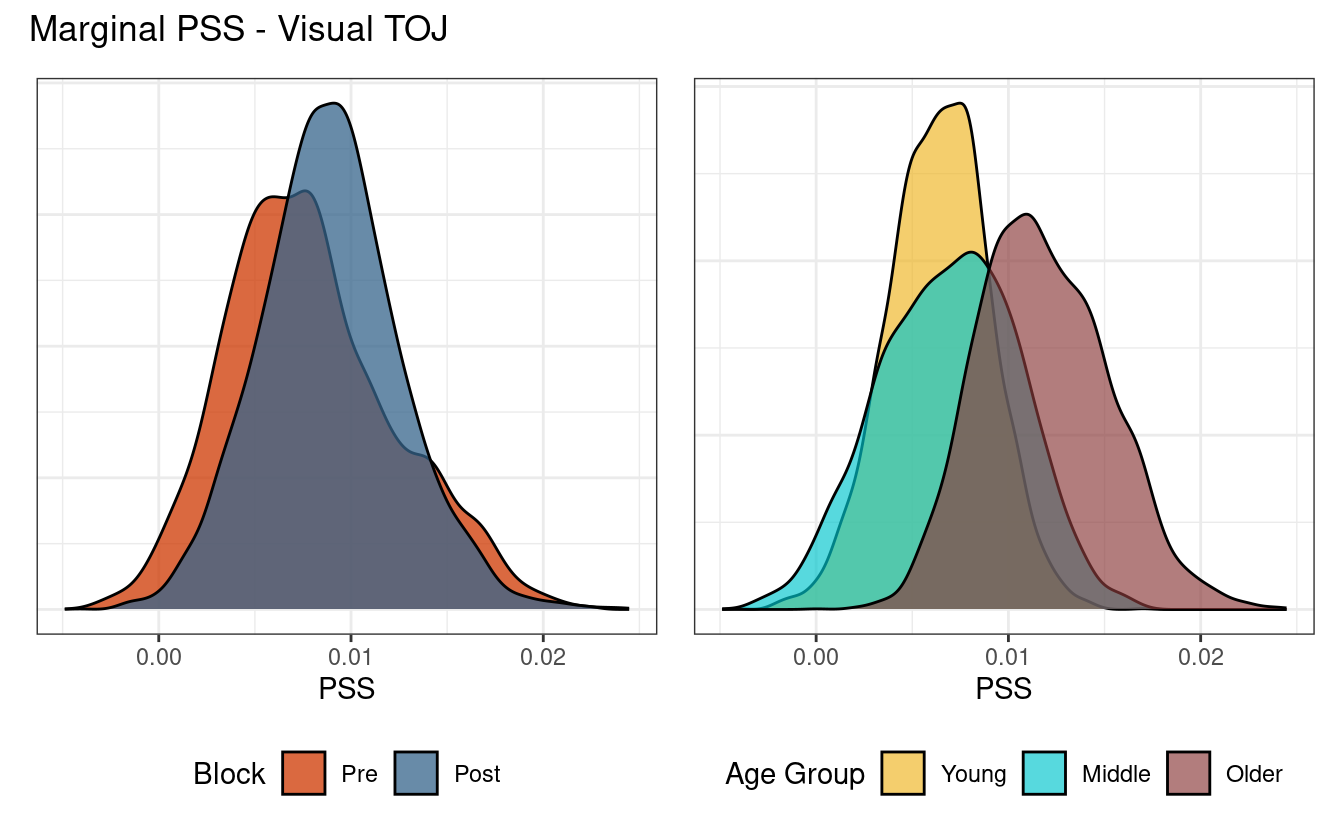
\includegraphics[width=0.85\linewidth]{050-results_files/figure-latex/ch050-Cold-Gamma-1} 

}

\caption{The difference between the older age group and the two others is noticeable, but not likely significant.}\label{fig:ch050-Cold-Gamma}
\end{figure}

These plots are useful for quickly being able to determine if there is a difference in factors. If there is a suspected difference, then the distribution can be calculated from the posterior samples as needed. We suspect that there may be a difference between the older age group and the other two, so we calculate the differences and summarize them with the histogram in figure \ref{fig:ch050-Rapid-Postal}.

\begin{figure}

{\centering 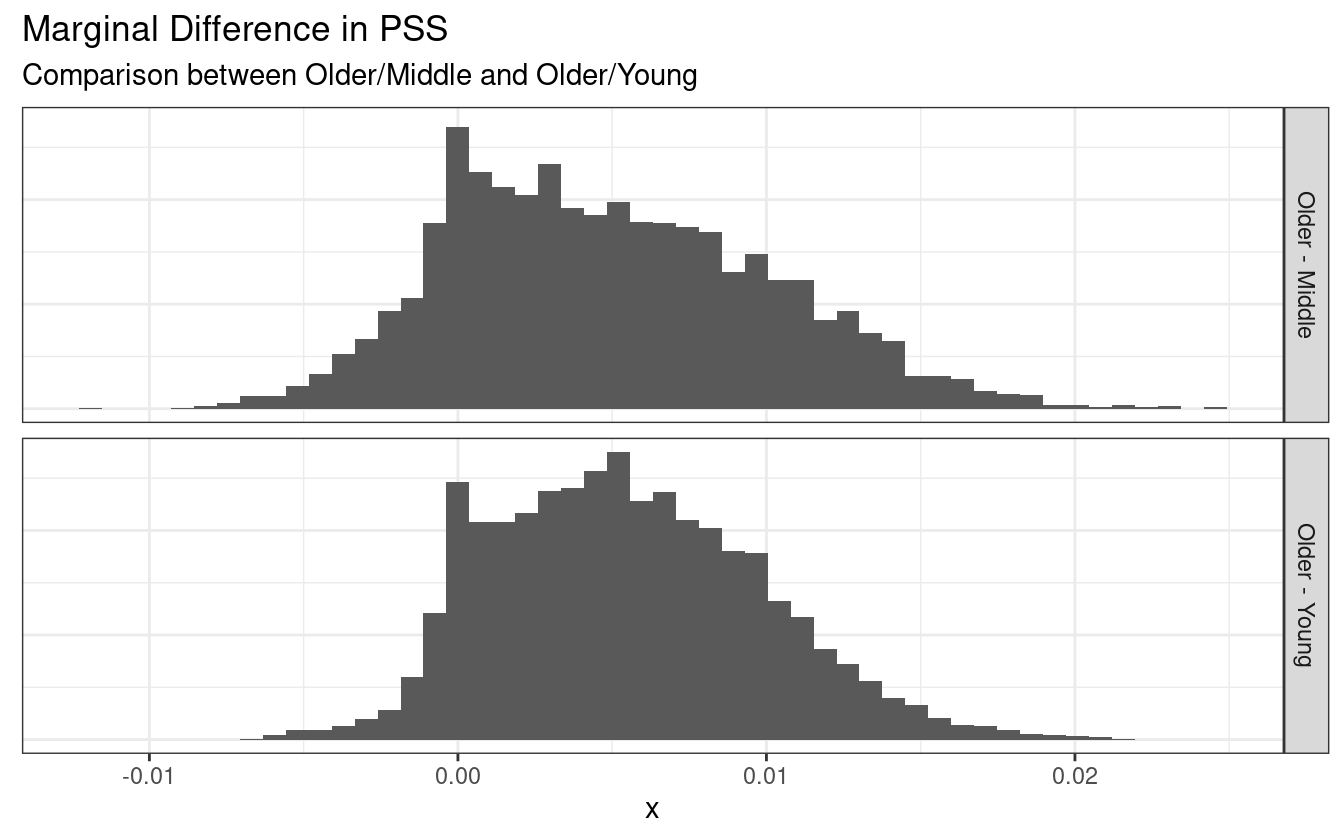
\includegraphics[width=0.85\linewidth]{050-results_files/figure-latex/ch050-Rapid-Postal-1} 

}

\caption{The bulk of the distribution is above zero, but there is still a chance that there is no difference in the distribution of PSS values between the age groups during the visual TOJ experiment.}\label{fig:ch050-Rapid-Postal}
\end{figure}

The bulk of the distribution is above zero, but there is still a chance that there is no difference in the distribution of PSS values between the age groups during the visual TOJ experiment.

\textbf{Duration TOJ Task}

\begin{figure}

{\centering 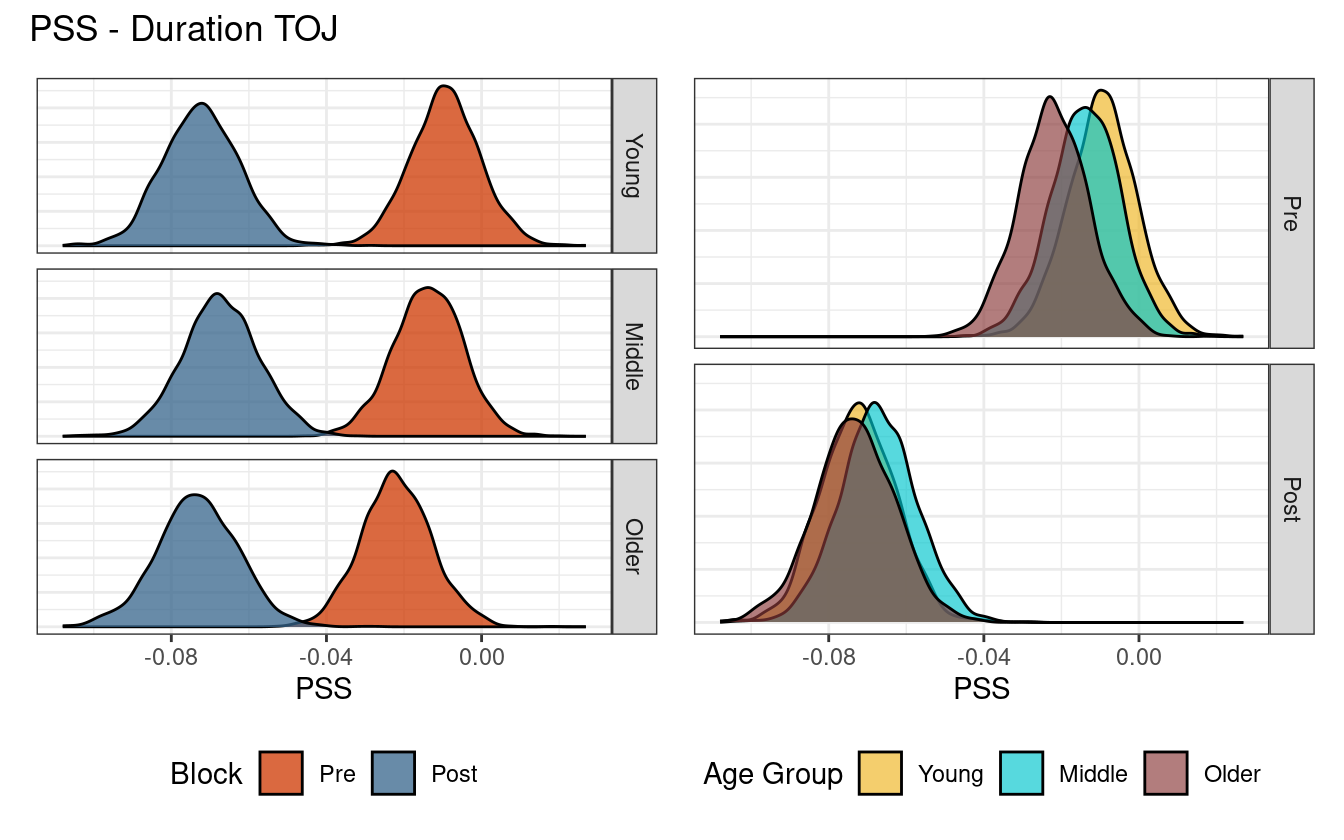
\includegraphics[width=0.85\linewidth]{050-results_files/figure-latex/ch050-Stormy-Frostbite-1} 

}

\caption{Posterior distribution of PSS values for the duration task.}\label{fig:ch050-Stormy-Frostbite}
\end{figure}

The duration TOJ task is very interesting because 1) recalibration had a visually significant effect across all age groups, and 2) there is virtually no difference between the age groups. We could plot the marginal distribution, but it would not give any more insight. What we might ask is what is it about the duration task that lets temporal recalibration have such a significant effect? Is human perception of time duration more malleable than our perception to other sensory signals?

\textbf{Sensorimotor TOJ Task}

\begin{figure}

{\centering 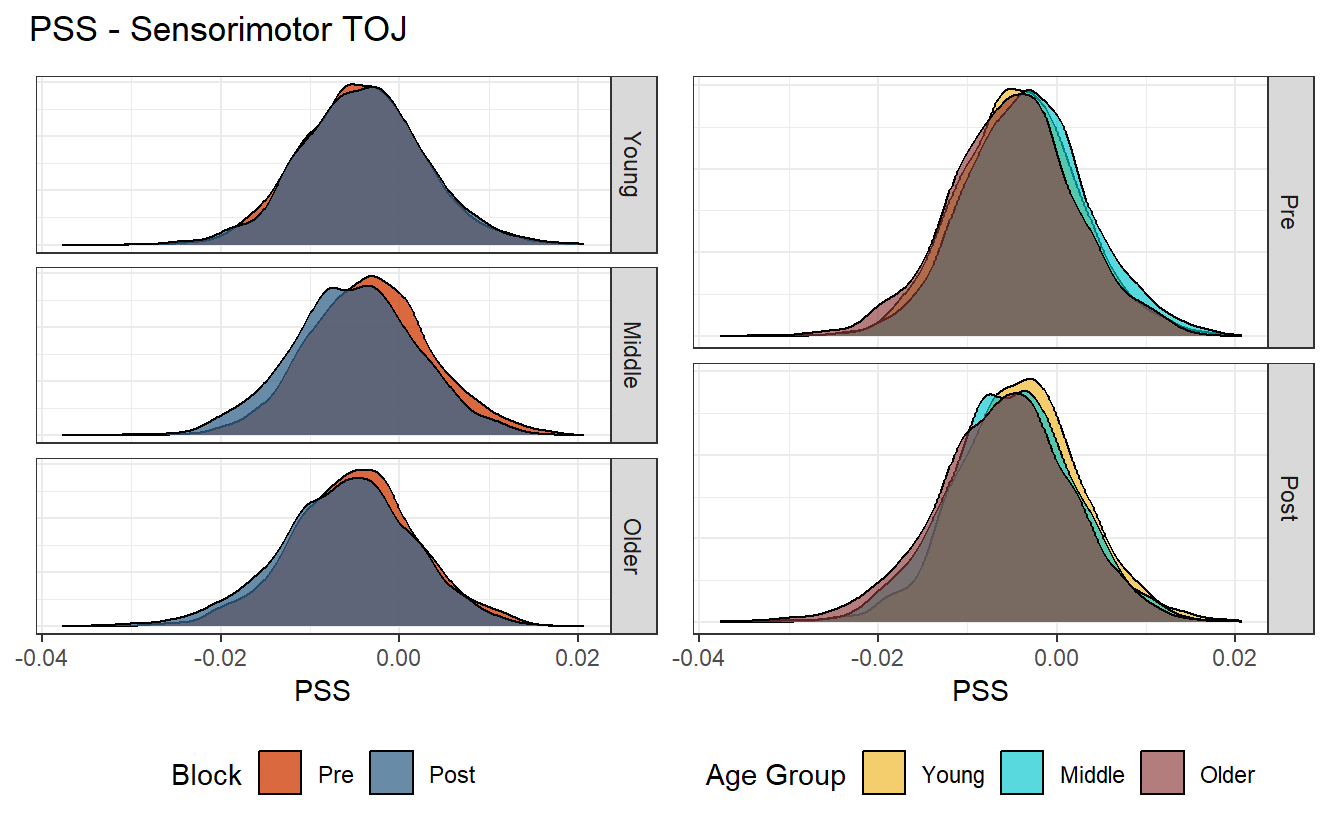
\includegraphics[width=0.85\linewidth]{050-results_files/figure-latex/ch050-Homeless-Anaconda-1} 

}

\caption{Posterior distribution of PSS values for the sensorimotor task.}\label{fig:ch050-Homeless-Anaconda}
\end{figure}

There are no differences between age groups or blocks when it comes to perceptual synchrony in the sensorimotor task.

\hypertarget{on-temporal-sensitivity}{%
\section{On Temporal Sensitivity}\label{on-temporal-sensitivity}}

Temporal sensitivity is the ability to successfully integrate signals arising from the same event, or segregate signals from different events. When the stimulus onset asynchrony increases, the ability to bind the signals into a single percept is reduced until they are perceived as distinct events with a temporal order. Those that are more readily able to determine temporal order have a higher temporal sensitivity, and it is measured through the slope of a psychometric function - specifically the quantity known as the just noticeable difference.

\textbf{Audiovisual TOJ Task}

\begin{figure}

{\centering 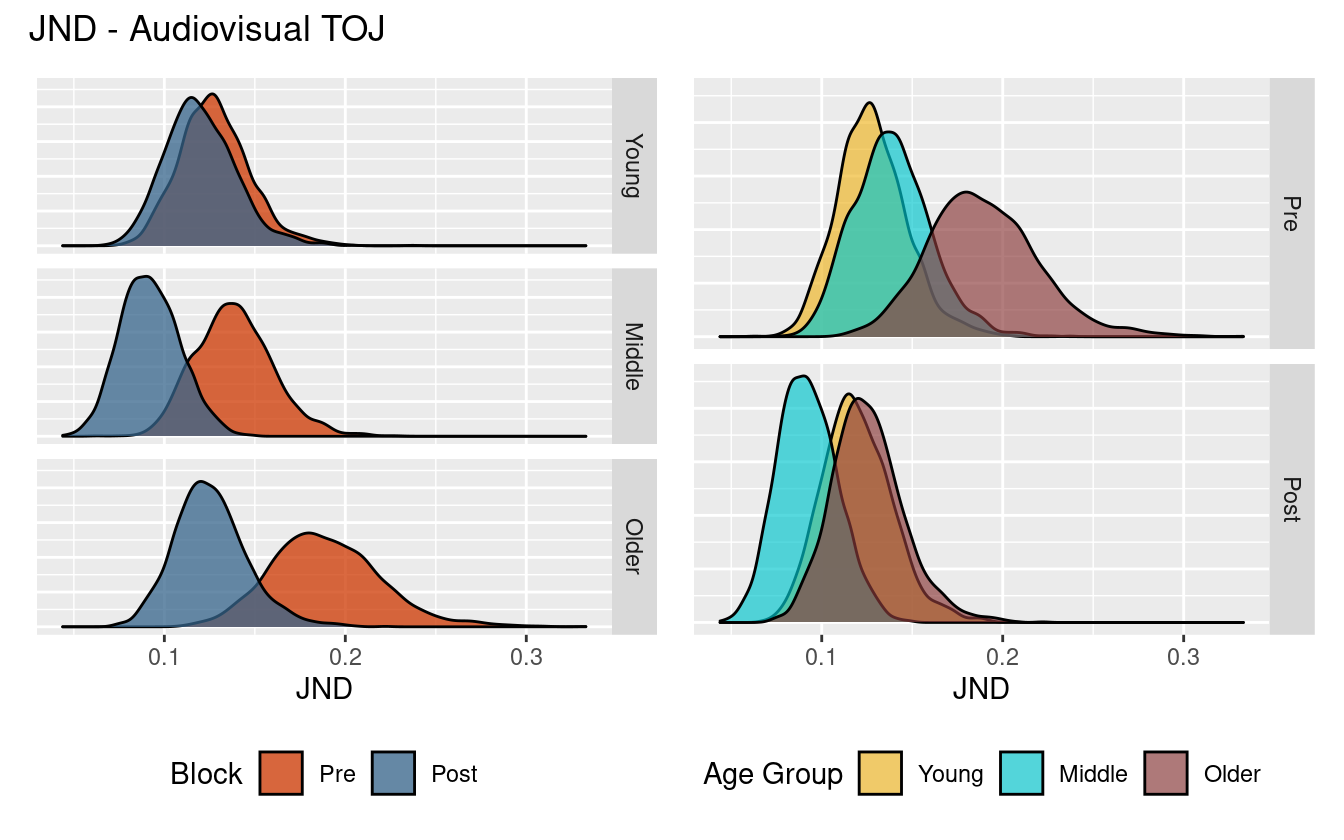
\includegraphics[width=0.85\linewidth]{050-results_files/figure-latex/ch050-Timely-Toupee-1} 

}

\caption{Posterior distribution of JND values for the audiovisual task.}\label{fig:ch050-Timely-Toupee}
\end{figure}

All age groups experienced an increase in temporal sensitivity, but the effect is largest in the older age group which also had the largest pre-adaptation JND estimates. There also appears to be some distinction between the older age group and the younger ones in the pre-adaptation block, but recalibration closes the gap.

\textbf{Visual TOJ Task}

\begin{figure}

{\centering 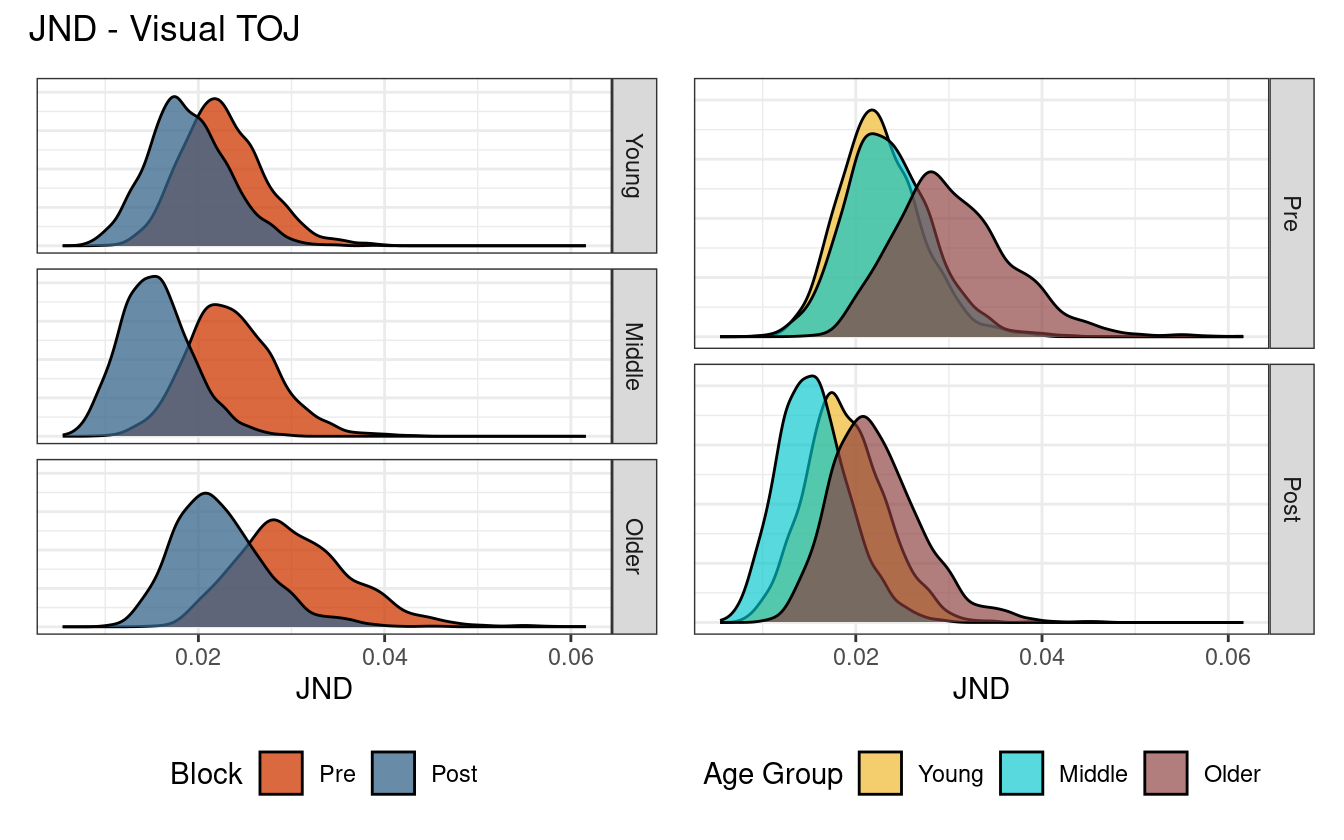
\includegraphics[width=0.85\linewidth]{050-results_files/figure-latex/ch050-Mercury-Rainbow-1} 

}

\caption{Posterior distribution of JND values for the visual task.}\label{fig:ch050-Mercury-Rainbow}
\end{figure}

The story for the visual TOJ task is similar to the audiovisual one - each age group experience heightened temporal sensitivity after recalibration, with the two older age groups receiving more benefit than the younger age group. It's also worth noting that the younger age groups have higher baseline temporal sensitivity, so there may not be as much room for improvement.

\textbf{Duration TOJ Task}

\begin{figure}

{\centering 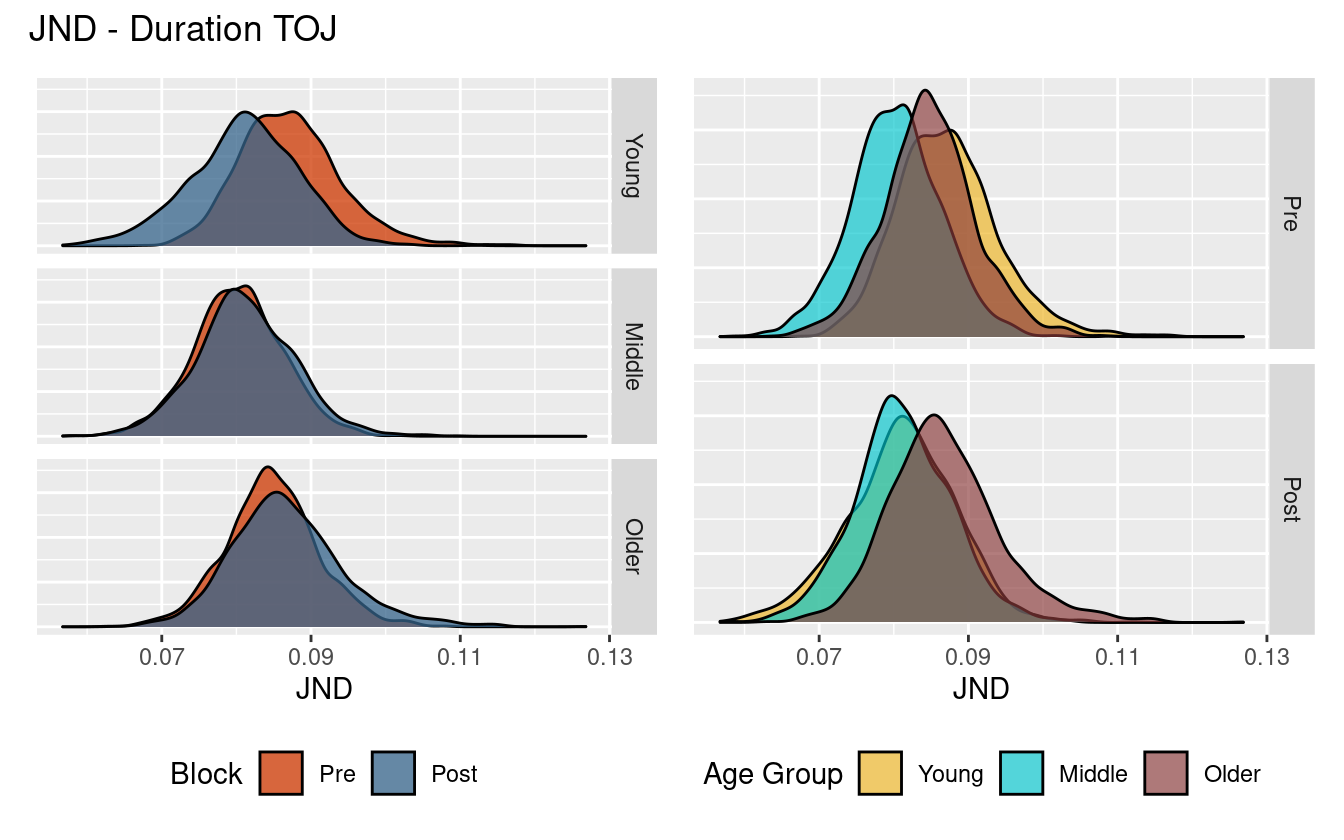
\includegraphics[width=0.85\linewidth]{050-results_files/figure-latex/ch050-Aimless-Planet-1} 

}

\caption{Posterior distribution of JND values for the duration task.}\label{fig:ch050-Aimless-Planet}
\end{figure}

This time the effects of recalibration are not so strong, and just like for the PSS, there is no significant difference between age groups in the duration task.

\textbf{Sensorimotor TOJ Task}

\begin{figure}

{\centering \includegraphics[width=0.85\linewidth]{050-results_files/figure-latex/ch050-Tombstone-Cold-1} 

}

\caption{Posterior distribution of JND values for the sensorimotor task.}\label{fig:ch050-Tombstone-Cold}
\end{figure}

Finally in the sensorimotor task there are mixed results. Temporal recalibration increased the temporal sensitivity in the younger age group, reduced it in the middle age group, and had no effect on the older age group. Clearly the biological factors at play are complex, and the data here is a relatively thin slice of the population. More data and a better calibrated experiment may give better insights into the effects of temporal recalibration.

\hypertarget{lapse-rate-across-age-groups}{%
\section{Lapse Rate across Age Groups}\label{lapse-rate-across-age-groups}}

\begin{figure}

{\centering \includegraphics[width=0.85\linewidth]{050-results_files/figure-latex/ch050-Waffle-Hollow-1} 

}

\caption{Process model of the result of a psychometric experiment with the assumption that lapses occur at random and at a fixed rate, and that the subject guesses randomly in the event of a lapse.}\label{fig:ch050-Waffle-Hollow}
\end{figure}

In the above figure, the outcome of one experiment can be represented as a directed acyclic graph (DAG) where at the start of the experiment, the subject either experiences a lapse in judgment with probability \(\gamma\) or they do not experience a lapse in judgment. If there is no lapse, then they will give a positive response with probability \(F(x)\). If there is a lapse in judgment, then it is assumed that they will respond randomly -- e.g.~a fifty-fifty chance of a positive response. In this model of an experiment, the probability of a positive response is the sum of the two paths.

\begin{align*}
\mathrm{P}(\textrm{positive}) &= 
  \mathrm{P}(\textrm{lapse}) \cdot \mathrm{P}(\textrm{positive} | \textrm{lapse}) \\
  &\quad + \mathrm{P}(\textrm{no lapse}) \cdot \mathrm{P}(\textrm{positive} | \textrm{no lapse}) \\
  &= \frac{1}{2} \gamma + (1 - \gamma) \cdot F(x)
\end{align*}

If we then let \(\gamma = 2\lambda\) then the probability of a positive response becomes

\[
\mathrm{P}(\textrm{positive}) = \lambda + (1 - 2\lambda) \cdot F(x)
\]

This is the same lapse model described in \eqref{eq:Psi}! But now there is more insight into what the parameter \(\lambda\) is. If \(\gamma\) is the true lapse rate, then \(\lambda\) is half the lapse rate. This may sound strange at first, but remember that equation \eqref{eq:Psi} was motivated as a lower and upper bound to the psychometric function where the bounds are constrained by the same amount. Here the motivation is from an illustrative diagram, yet the two lines of reasoning arrive at the same model.

Figure \ref{fig:ch050-Magenta-Finger} shows the distribution of lapse rates for each age group across the four separate tasks. There is no visual trend in the ranks of lapse rates, meaning that no single age group definitively experiences a lower lapse rate than the others, though the middle age group comes close to being the winner and the older age group is more likely to be trailing behind. The distribution of lapse rates does reveal something about the tasks themselves.

\begin{figure}

{\centering \includegraphics[width=0.85\linewidth]{050-results_files/figure-latex/ch050-Magenta-Finger-1} 

}

\caption{Lapse rates for the different age groups across the four separate tasks. Visually there is no clear trend in lapses by age group, but the concentration of the distributions give insight into the perceived difficulty of a task where more diffuse distributions may indiciate more difficult tasks.}\label{fig:ch050-Magenta-Finger}
\end{figure}

We used the audiovisual data in the first few iterations of building a model and there were no immediate issues, but when we tested the model on the visual data it had trouble expressing the variability at outer SOA values. We also noted that one subject had a near perfect response set, and many others had equally impressive performance. The model without a lapse rate was being torn between a very steep slope near the PSS and random variability near the outer SOAs. The remedy was to include a lapse rate (motivated by domain expertise) which allowed for that one extra degree of freedom necessary to reconcile the opposing forces.

Why did the visual data behave this way when the audiovisual data had no issue? That gets deep into the theory of how our brains integrate signals arising from different modalities. Detecting the temporal order of two visual stimuli may be an easier mental task than that of heterogeneous signals. Then consider the audiovisual task versus the duration or sensorimotor task. Visual-speech synthesis is a much more common task throughout the day than visual-tactile (sensorimotor), and so perhaps we are better adjusted to such a task as audiovisual. The latent measure of relative performance or task difficulty might be picked up through the lapse rate.

To test this idea, the TOJ experiment could be repeated, but also ask the subject afterwards how they would rate the difficulty of each task. For now, a post-hoc test can be done by comparing the mean and spread of the lapse rates to a pseudo-difficulty measure as defined by the proportion of the incorrect responses. A response is correct when the sign of the SOA value is concordant with the response, e.g.~a positive SOA and the subject gives the ``positive'' response or a negative SOA and the subject gives the ``negative'' response. Looking at figure \ref{fig:ch050-Magenta-Finger}, we would subjectively rate the tasks from easiest to hardest based on ocular analysis as

\begin{enumerate}
\def\labelenumi{\arabic{enumi}.}
\tightlist
\item
  Visual
\item
  Audiovisual
\item
  Duration
\item
  Sensorimotor
\end{enumerate}

Again, this ranking is based on the mean (lower intrinsically meaning easier) and the spread (less diffuse implying more agreement of difficulty between age groups). The visual task has the tightest distribution of lapse rates, and the sensorimotor has the widest spread, so we can rank those first and last respectively. Audiovisual and duration are very similar in mean and spread, but the audiovisual has a bit more agreement between the young and middle age groups, so second and third go to audiovisual and duration. Table \ref{tab:ch050-Orange-Tigerfish} shows the results arranged by increasing pseudo difficulty. As predicted, the visual task is squarely at the top and the sensorimotor is fully at the bottom. The only out of place group is the audiovisual task for the older age group, which is about equal to the older age group during the duration task. In fact, within tasks, the older age group always comes in last in terms of proportion of correct responses, while the young and middle age groups trade back and forth.

\begin{table}[!h]

\caption{\label{tab:ch050-Orange-Tigerfish}Relative difficulty of the different tasks by age group. The difficulty is measured by the proportion of incorrect responses.}
\centering
\begin{tabular}[t]{llr}
\toprule
Task & Age Group & Pseudo Difficulty\\
\midrule
visual & Middle & 0.03\\
visual & Young & 0.03\\
visual & Older & 0.06\\
audiovisual & Young & 0.12\\
audiovisual & Middle & 0.12\\
\addlinespace
duration & Middle & 0.14\\
duration & Young & 0.16\\
duration & Older & 0.17\\
audiovisual & Older & 0.17\\
sensorimotor & Young & 0.22\\
\addlinespace
sensorimotor & Middle & 0.24\\
sensorimotor & Older & 0.29\\
\bottomrule
\end{tabular}
\end{table}

\hypertarget{subject-specific-inferences}{%
\section{Subject specific inferences}\label{subject-specific-inferences}}

The multilevel model described by \eqref{eq:iter5-model} provides subject-specific estimation as well as the age group level estimations presented above. If desired, we can make comparisons between subjects or use the subject level estimates to highlight the variation within age groups. Figure \ref{fig:ch050-Green-Metaphor} shows the comparison of two middle aged subjects from the visual TOJ task. They both show heightened temporal sensitivity through an increased slope.

\begin{figure}

{\centering \includegraphics[width=0.85\linewidth]{figures/ch050-Green-Metaphor} 

}

\caption{Comparison of subject-specific distribution of psychometric functions from the Visual TOJ task.}\label{fig:ch050-Green-Metaphor}
\end{figure}

The subject-level model can make predictions for new individuals or for individuals that did not complete a block. Recall that the post-adaptation block for subject \texttt{O-f-CE} was removed from the audiovisual data set (see figure \ref{fig:ch020-av-post1-O-f-CE-plot}). We can still predict their post-adaptation performance because we have information from their pre-adaptation responses and the age-block level estimates as demonstrated in figure \ref{fig:ch050-Solid-Autumn}.

\begin{figure}

{\centering \includegraphics[width=0.85\linewidth]{figures/ch050-Solid-Autumn} 

}

\caption{Block estimates for subject `O-f-CE`. Even though their post-adaptation block was not in the data set, we can make predtictions thanks to the multilevel model with subject-level predictors.}\label{fig:ch050-Solid-Autumn}
\end{figure}

\hypertarget{conclusion}{%
\chapter{Discussion and Conclusion}\label{conclusion}}

The results from the previous chapter provide insight into how future experiments can be designed to offer better inferences. In the visual TOJ task, the granularity in the SOA values near the PSS could be increased to get more reliable estimates of the slope and to avoid complete separation. Including a lapse rate helps, but can be unreliable if the range of SOA values is too narrow. For more difficult tasks like the sensorimotor TOJ task, larger SOA values are necessary so that the lapse rate can be accurately measured.

The results presented previously are based off of a small scale preliminary data set, so there's a lot of uncertainty in the measure of the psychometric quantities. One way to remove the uncertainty of the lapse rate could be to have some trials with very large SOA values. The reasoning is that if the difficulty of a task (given an SOA value) is lowered, than an incorrect response is more likely to be correctly attributed to a true lapse in judgment as opposed to a genuinely incorrect response. \citet{wichmann2001b} recommends at least one sample at \(\pi \ge 0.95\) is necessary for reliable bootstrap confidence intervals, so the same reasoning can be applied when using Bayesian credible intervals. For a task such as visual TOJ, the \(90\%\) level may occur at an SOA of \(\approx 40\)ms while for the audiovisual TOJ it may be \(\approx 220\)ms, so the sampling scheme for psychometric experiments must be tuned to the task.

\citet{wichmann2001a} experimentally determined that the lapse rate for trained observers is between \(0\%\) and \(5\%\), and the data in this paper loosely agree with that conclusion. Any excess in lapse rate may be attributed to the perceived task difficulty and a sub-optimal sampling scheme. Since the visual TOJ task is relatively the easiest, the estimated lapse rates are more believable as true lapse rates, and fall closely within the \((0, 0.05)\) range. Since the lapse rate is estimated to be no more than \(0.05\), an experiment would need about \(20\) trials at a larger SOA in order to pick up on a single lapse. In this data, we have multiple subjects within an age group, so the repetition is spread out. As a consequence, it is possible to estimate an age group level lapse rate, but more difficult to estimate subject specific lapses.

For multilevel modeling and partial pooling to have a significant benefit, five or more groups is recommended. The study could be expanded to have five or six age groups (20-30, 30-40, etc.). More age groups would also allow for finer tracking of trends in the distribution of PSS and JND values and the affect of temporal recalibration on them.

In the future we would like to explore a causal inference model for the psychometric function. The results drawn from the statistical model are simply associations between the predictor variables, and of course correlations do not imply causation. How do we move from association to cause-and-effect? Drawing the model as a directed acyclic graph and testing the implications of the model is a start. With a proper model, total effects of a certain variable on the outcome can be determined.

The model development was motivated by domain expertise consistency and the model's ability to answer domain-related research questions. The emphasis is on model comparison which is not necessarily model selection. Certain models are useful for answering different questions. We compared models that have the potential to answer questions pertaining to the age group level and compared their estimated predictive performance. Predictive performance is a reliable metric for model comparison because a model that can predict well likely captures the regular features of the observed data and the data generating model.

We have produced a novel statistical model for temporal order judgment data by following a principled workflow and fitting a series of Bayesian models efficiently using Hamiltonian Monte Carlo in the \texttt{R} programming language with \texttt{Stan}. We described methods for selecting priors for the slope and intercept parameters, and argued why the selected linear parameterization can have practical benefits on prior specification. Finally we motivated the inclusion of a lapse rate into the model for the psychometric function with an illustrative diagram of the result of a temporal order judgment experiment.

\hypertarget{appendix-appendix}{%
\appendix}


\hypertarget{code}{%
\chapter{Supplementary Code}\label{code}}

\textbf{Eight Schools Model}

\setstretch{1.0}

\begin{verbatim}
data {
  int<lower=0> J;         // number of schools 
  real y[J];              // estimated treatment effects
  real<lower=0> sigma[J]; // standard error of effect estimates 
}
parameters {
  real mu;                // population treatment effect
  real<lower=0> tau;      // standard deviation in treatment effects
  vector[J] eta;          // unscaled deviation from mu by school
}
transformed parameters {
  vector[J] theta = mu + tau * eta; // school treatment effects
}
model {
  target += normal_lpdf(eta | 0, 1);       // prior log-density
  target += normal_lpdf(y | theta, sigma); // log-likelihood
}
generated quantities {
  vector[J] log_lik;

  for (j in 1:J) {
    log_lik[j] = normal_lpdf(y[j] | theta[j], sigma[j]);
  }
}
\end{verbatim}

\setstretch{2.0}

\clearpage

\textbf{Model with Lapse and Subject-level Parameters}

\setstretch{1.0}

\begin{verbatim}
data {
  int N;        // Number of observations
  int N_G;      // Number of age groups
  int N_T;      // Number of treatments
  int N_S;      // Number of subjects
  int n[N];     // Number of Bernoulli trials
  int k[N];     // Number of "positive" responses
  vector[N] x;  // SOA values
  int G[N];     // Age group index variable
  int trt[N];   // Treatment index variable
  int S[N];     // Subject index variable
}
parameters {
  real a_raw;
  real<lower=machine_precision(),upper=pi()/2> aGT_unif;
  real<lower=machine_precision(),upper=pi()/2> aS_unif;
  matrix[N_G, N_T] aGT_raw;
  vector[N_S] aS_raw;

  real b_raw;
  real<lower=machine_precision(),upper=pi()/2> bGT_unif;
  real<lower=machine_precision(),upper=pi()/2> bS_unif;
  matrix[N_G, N_T] bGT_raw;
  vector[N_S] bS_raw;

  vector[N_G] lG;
}
transformed parameters {
  real a;
  matrix[N_G, N_T] aGT;
  vector[N_S] aS;
  real sd_aGT;
  real sd_aS;

  real b;
  matrix[N_G, N_T] bGT;
  vector[N_S] bS;
  real sd_bGT;
  real sd_bS;

  a = a_raw * 0.06;
  sd_aGT = tan(aGT_unif);
  sd_aS  = tan(aS_unif);
  aS = aS_raw * sd_aS;

  b = 3.0 + b_raw;
  sd_bGT = 2 * tan(bGT_unif);
  sd_bS  = 2 * tan(bS_unif);
  bS = bS_raw * sd_bS;

  for (i in 1:N_G) {
    for (j in 1:N_T) {
      aGT[i, j] = aGT_raw[i, j] * sd_aGT;
      bGT[i, j] = bGT_raw[i, j] * sd_bGT;
    }
  }
}
model {
  vector[N] p;

  a_raw ~ std_normal();
  b_raw ~ std_normal();
  lG ~ beta(4, 96);

  aS_raw ~ std_normal();
  bS_raw ~ std_normal();
  to_vector(aGT_raw) ~ std_normal();
  to_vector(bGT_raw) ~ std_normal();

  for (i in 1:N) {
    real alpha = a + aGT[G[i], trt[i]] + aS[S[i]];
    real beta = b + bGT[G[i], trt[i]] + bS[S[i]];
    real lambda = lG[G[i]];
    p[i] = lambda + (1 - 2*lambda) * inv_logit(exp(beta) * (x[i] - alpha));
  }

  k ~ binomial(n, p);
}
generated quantities {
  vector[N] log_lik;
  vector[N] k_pred;

  for (i in 1:N) {
    real alpha = a + aGT[G[i], trt[i]] + aS[S[i]];
    real beta  = b + bGT[G[i], trt[i]] + bS[S[i]];
    real lambda = lG[G[i]];

    real p = lambda + (1 - 2*lambda) * inv_logit(exp(beta) * (x[i] - alpha));

    log_lik[i] = binomial_lpmf(k[i] | n[i], p);
    k_pred[i]  = binomial_rng(n[i], p);
  }
}
\end{verbatim}

\setstretch{2.0}

\clearpage

\textbf{Stan Algebraic Solver}

\setstretch{1.0}

\begin{verbatim}
functions {
  vector system(vector y, vector theta, real[] x_r, int[] x_i) {
    vector[2] z;
    z[1] = exp(y[1] + y[2]^2 / 2) - theta[1];
    z[2] = 0.5 + 0.5 * erf(-y[1] / (sqrt(2) * y[2])) - theta[2];
    return z;
  }
}
transformed data {
  vector[2] y_guess = [1, 1]';
  real x_r[0];
  int x_i[0];
}
transformed parameters {
  vector[2] theta = [0.100, 0.99]';
  vector[2] y;
  y = algebra_solver(system, y_guess, theta, x_r, x_i);
}
\end{verbatim}

\setstretch{2.0}

\hypertarget{model-dev}{%
\chapter{Developing a Model}\label{model-dev}}

Our final modeling strategy is an evolution from other attempts. The development proceeded through multiple iterations described in \protect\hyperlink{application}{chapter 4}, but doesn't tell the full story. We learn more from others when they share what didn't work along with the final path that did work. There is knowledge to be gained in failed experiments, because then there is one more way to not do something, just like a failing outcome reduces the variance of the Beta distribution.

In the first attempt at modeling, we used a classical GLM to get a baseline understanding of the data, but the fact that some estimates for certain subjects failed due to complete separation reinforced the our adoption of non-classical techniques. Our first Bayesian model was derived from \citet{lee2014bayesian} which used nested loops to iterate over subjects and SOA values. The data were required to be stored in a complicated way that made it difficult to comprehend and extend.

We moved on to using \texttt{arm::bayesglm} to remove convergence issues, but we were met with other limitations such as linear parameterization and lack of hierarchical modeling. The book Statistical Rethinking \citep{mcelreath2020statistical} offers a great first introduction to Bayesian multilevel modeling. McElreath's \texttt{rethinking} package accompanies the book, and offers a compact yet expressive syntax for models that get translated into a Stan model. A model with age group and block can be written using \texttt{rethinking::ulam} as

\setstretch{1.0}

\begin{Shaded}
\begin{Highlighting}[]
\NormalTok{rethinking}\SpecialCharTok{::}\FunctionTok{ulam}\NormalTok{(}\FunctionTok{alist}\NormalTok{(}
\NormalTok{  k }\SpecialCharTok{\textasciitilde{}} \FunctionTok{binomial\_logit}\NormalTok{(n, p),}
  \AttributeTok{p =} \FunctionTok{exp}\NormalTok{(b }\SpecialCharTok{+}\NormalTok{ bG[G] }\SpecialCharTok{+}\NormalTok{ bT[trt]) }\SpecialCharTok{*}\NormalTok{ (x }\SpecialCharTok{{-}}\NormalTok{ (a }\SpecialCharTok{+}\NormalTok{ aG[G] }\SpecialCharTok{+}\NormalTok{ aT[trt])),}
\NormalTok{  a }\SpecialCharTok{\textasciitilde{}} \FunctionTok{normal}\NormalTok{(}\DecValTok{0}\NormalTok{, }\FloatTok{0.06}\NormalTok{),}
\NormalTok{  aG[G] }\SpecialCharTok{\textasciitilde{}} \FunctionTok{normal}\NormalTok{(}\DecValTok{0}\NormalTok{, sd\_aG),}
\NormalTok{  aT[trt] }\SpecialCharTok{\textasciitilde{}} \FunctionTok{normal}\NormalTok{(}\DecValTok{0}\NormalTok{, sd\_aT),}
\NormalTok{  b }\SpecialCharTok{\textasciitilde{}} \FunctionTok{normal}\NormalTok{(}\DecValTok{3}\NormalTok{, }\DecValTok{1}\NormalTok{),}
\NormalTok{  bG[G] }\SpecialCharTok{\textasciitilde{}} \FunctionTok{normal}\NormalTok{(}\DecValTok{0}\NormalTok{, sd\_bG),}
\NormalTok{  bT[trt] }\SpecialCharTok{\textasciitilde{}} \FunctionTok{normal}\NormalTok{(}\DecValTok{0}\NormalTok{, sd\_bT),}
  \FunctionTok{c}\NormalTok{(sd\_aG, sd\_aT, sd\_bG, sd\_bT) }\SpecialCharTok{\textasciitilde{}} \FunctionTok{half\_cauchy}\NormalTok{(}\DecValTok{0}\NormalTok{, }\DecValTok{5}\NormalTok{)}
\NormalTok{), }\AttributeTok{data =}\NormalTok{ df, }\AttributeTok{chains =} \DecValTok{4}\NormalTok{, }\AttributeTok{cores =} \DecValTok{4}\NormalTok{, }\AttributeTok{log\_lik =} \ConstantTok{TRUE}\NormalTok{)}
\end{Highlighting}
\end{Shaded}

\setstretch{2.0}

While learning about multilevel models, we tried writing a package that generates a \texttt{Stan} program based on \texttt{R} formula syntax. At the time the concepts of no-pooling, complete pooling, and partial pooling were vaguely understood, and the package was plagued by the same lack of flexibility that \texttt{rstanarm} and \texttt{brms} have. Then it was discovered that \texttt{brms} and \texttt{rstanarm} already did what we were trying to do, but programming experience was invaluable.

We also tried using \texttt{lme4}, \texttt{rstanarm}, and \texttt{brms}, and learned more about the concepts of fixed and random effects. We noticed that parameterization can have a significant affect on the efficiency of a model and the inferential power of the estimated parameters. When fitting a classical model, there is little difference in estimating \texttt{a\ +\ bx} vs.~\texttt{d(x\ -\ c)} since the latter can just be expanded as \texttt{-cd\ +\ dx} which is essentially the same as the first parameterization, but there is a practical difference in the interpretation of the parameters. The second parameterization implies that there is a dependence among the parameters that can be factored out. In the context of psychometric functions, there is a stronger connection between PSS and \texttt{c} and the JND and \texttt{d}. This parameterization made it easier to specify priors and also increased the model efficiency. Of the modeling tools mentioned, only \texttt{rethinking} and \texttt{Stan} allow for arbitrary parameterization.

We finally arrived at a model that worked well, but learned that using a binary indicator variable for the treatment comes with the assumption of higher uncertainty for one of the conditions. The linear model that we arrived at is displayed in equation \eqref{eq:badlinearmodel}.

\begin{equation}
  \theta = \exp(\beta + \beta_G +(\beta_T + \beta_{TG})\times trt) \left[x - (\alpha + \alpha_G + (\alpha_T + \alpha_{TG})\times trt)\right]
  \label{eq:badlinearmodel}
\end{equation}

Using an indicator variable in this fashion also introduced an interaction effect into the model that we almost did not account for after switching to using a factor variable. Interaction effects between factors is handled by creating a new factor that is essentially the cross-product of other factor variables. E.g. for factor variables \(x\) and \(y\)

\setstretch{1.0}

\[
x = \begin{bmatrix}
a \\
b \\
c
\end{bmatrix}, y =  \begin{bmatrix}
i \\
j
\end{bmatrix}\Longrightarrow x\times y = 
\begin{bmatrix}
ai & aj \\
bi & bj \\
ci & cj
\end{bmatrix}
\]
\setstretch{2.0}

The final round of reparameterization came in the form of adopting non-centered parameterization for more efficient models. To us, \(Z \sim N(0, 1^2);\quad X = 3 + 2Z\) is the same as \(X \sim N(3, 2^2)\), but to a computer the process of sampling from \(X\) can be more difficult than sampling from \(Z\) (discussed in \protect\hyperlink{methods}{chapter 2}).

\hypertarget{reproduce}{%
\chapter{Reproducible Results}\label{reproduce}}

Data doesn't always come in a nice tidy format, and we had to turn the raw experimental data into a clean data set that is ready for modeling. Sometimes the process is quick and straight forward, but other times, like with this psychometric data, it takes more effort and clever techniques. There is academic value in describing the steps taken to reduce the headache later.

To begin, there is a strong push in recent years for reproducible data science. Scientific methods and results should be able to be replicated by other researchers, and part of that includes being able to replicate the process that takes the raw data and produces the tidy data that is ready for analysis. Tidy data is described by \citet{wickham2014tidy} and can be summed up by three principles

\setstretch{1.0}

\begin{enumerate}
\def\labelenumi{\arabic{enumi}.}
\tightlist
\item
  Each variable forms a column
\item
  Each observation forms a row
\item
  Each type of observational unit forms a table
  \setstretch{2.0}
\end{enumerate}

One problem is having data in a spread sheet, modifying it, and then having no way of recovering the original data. Spread sheets are a convenient way to organize, transform, and lightly analyze data, but problems can quickly arise unless there is a good backup/snapshot system in place. Mutability in computer science is the property of a data structure where its contents can be modified in place. Immutability means that the object cannot be modified without first making a copy. Data is immutable, or at least that is the mindset that researchers must adopt in order to have truly reproducible workflows. The raw data that is collected or produced by a measurement device should never be modified without first being copied, even if for trivial reasons such as correcting a spelling mistake. If a change is made to the raw data, it should be carefully documented and reversible.

To begin the data cleaning journey, we introduce the directory system that we had been given to work with. Each task is separated into its own folder, and within each folder is a subdirectory of age groups.

\begin{figure}

{\centering \includegraphics[width=0.3\linewidth]{figures/data_dir} 

}

\caption{Top-level data directory structure.}\label{fig:ch230-Lama-Everyday}
\end{figure}

Within each age group subdirectory are the subdirectories for each subject named by their initials which then contain the experimental data in Matlab files.

\begin{figure}

{\centering \includegraphics[width=0.35\linewidth]{figures/data_subdir} 

}

\caption{Subdirectory structure.}\label{fig:ch230-Third-Needless-Antique}
\end{figure}

The data appears manageable, and there is information contained in the directory structure such as task, age group, and initials, and file name contains information about the experimental block. There is also an excel file that we were later given that contains more subject information like age and sex, though that information is not used in the model. The columns of the Matlab file depend on the task, but generally they contain an SOA value and a response, but no column or row name information -- that was provided by the researcher who collected the data.

We then created a table of metadata -- information extracted from the directory structure and file names combined with the the subject data and the file path. Regular expressions can be used to extract patterns from a string. With a list of all Matlab files within the \texttt{RecalibrationData} folder, we tried to extract the task, age group, initials, and block using the regular expression:

\begin{verbatim}
"^(\\w+)/(\\w+)/(\\w+)/[A-Z]{2,3}_*[A-Z]*(adapt[0-9]|baseline[0-9]*).*"
\end{verbatim}

The \texttt{\^{}(\textbackslash{}\textbackslash{}w+)/} matches any word characters at the start and before the next slash. Since the directory is structured as \texttt{Task/AgeGroup/Subject/file.mat}, the regular expression should match three words between slashes. The file name generally follows the pattern of \texttt{Initials\_\_block\#\_\_MAT.mat}, so \texttt{{[}A-Z{]}\{2,3\}\_*{[}A-Z{]}*} should match the initials, and \texttt{(adapt{[}0-9{]}\textbar{}baseline{[}0-9{]}*)} should match the block (baseline or adapt). This method works for \(536\) of the \(580\) individual records. For the ones it failed, it was generally do to misspellings or irregular capitalizing of ``baseline'' and ``adapt''.

Since there is only a handful of irregular block names, they can be dealt with by a separate regular expression that properly extracts the block information. Other challenges in cleaning the data include the handling of subjects with the same initials. This becomes a problem when filtering by a subject's initials is not guaranteed to return a unique subject. Furthermore there are two middle age subjects with the same initials of ``JM'', so one was also identified with their sex ``JM\_F''. The solution is to create a unique identifier (labeled as SID) that is a combination of age group, sex, and initials. For an experiment identifier (labeled as RID), the task and block were prepended to the SID. Each of these IDs uniquely identify the subjects and their experimental records making it easier to filter and search.

\setstretch{1.0}

\begin{Shaded}
\begin{Highlighting}[]
\FunctionTok{glimpse}\NormalTok{(features, }\AttributeTok{width =} \DecValTok{60}\NormalTok{)}
\CommentTok{\#\textgreater{} Rows: 580}
\CommentTok{\#\textgreater{} Columns: 8}
\CommentTok{\#\textgreater{} $ rid       \textless{}fct\textgreater{} av{-}post1{-}M{-}f{-}CC, av{-}post1{-}M{-}f{-}DB, av{-}pos\textasciitilde{}}
\CommentTok{\#\textgreater{} $ sid       \textless{}fct\textgreater{} M{-}f{-}CC, M{-}f{-}DB, M{-}f{-}HG, M{-}f{-}JM, M{-}f{-}MS, \textasciitilde{}}
\CommentTok{\#\textgreater{} $ path      \textless{}chr\textgreater{} "Audiovisual/MiddleAge/CC/CCadapt1\_\_MAT.\textasciitilde{}}
\CommentTok{\#\textgreater{} $ task      \textless{}chr\textgreater{} "audiovisual", "audiovisual", "audiovisu\textasciitilde{}}
\CommentTok{\#\textgreater{} $ trial     \textless{}fct\textgreater{} post1, post1, post1, post1, post1, post1\textasciitilde{}}
\CommentTok{\#\textgreater{} $ age\_group \textless{}fct\textgreater{} middle\_age, middle\_age, middle\_age, midd\textasciitilde{}}
\CommentTok{\#\textgreater{} $ age       \textless{}dbl\textgreater{} 39, 44, 41, 48, 49, 43, 47, 49, 49, 44, \textasciitilde{}}
\CommentTok{\#\textgreater{} $ sex       \textless{}fct\textgreater{} F, F, F, F, F, F, F, F, F, M, M, M, M, M\textasciitilde{}}
\end{Highlighting}
\end{Shaded}

\setstretch{2.0}

Then with the table of clean metadata, the task is simply to loop through each row, read the Matlab file given by \texttt{path}, add the unique ID as a column, and then join the experimental data with the metadata to create a data set that is ready for model fitting and data exploration. The full code used to generate the clean data is not yet available online, but can be shared with the committee.

The benefit of writing a script to generate the data is that others can look over the code and verify that it is doing what it is intended to do, and we can go back to any step within the process to make changes if the need comes up. Another tool that contributed to the reproducibility is the version control management software, Git. With Git we can take a snapshot of the changes made, and revert if necessary. This thesis is also hosted on Github, and the entire history of development can be viewed there.
%==============================================================================26
\backmatter
%==============================================================================27
\bibliography{bibliography.bib,packages.bib}
%==============================================================================28
% Place here anything that you would like to come
% after the appendix, references, etc
%==============================================================================29
\end{document}
